\chapter{CSDL Study} \label{Chapter:EvaluationInCSDL}


The previous chapter reported on a classroom study of software project telemetry. The classroom study has the advantage of obtaining insights from a relatively large number of people in a relatively short period of time.  However, it has a number of limitations: the size and the scope of the class projects were relatively small, the time the students could devote to software development activities was relatively limited, and the students in classroom tend to have less software engineering experience.
To mitigate the limitations, I performed another study in the Collaborative Software Development Lab (CSDL) during Spring 2006. The CSDL study had a number of complementary characteristics to the classroom study. Though it involved only five developers and one project manager, the system under development was much larger in scale with almost 300,000 lines of code in total. It had been under development for five years. The CSDL developers had significantly more software engineering experience compared to the developers in the classroom on average. 
Instead of a one-shot survey, I pursued a much more in-depth data collection and analysis strategy over a much longer period of time. 
While still within an academic setting, it intends to provide data that reflect an environment much closer to those in industrial settings.

%In the CSDL study, I introduced software project telemetry as a metrics-based software process improvement program. 

%But before going into details, I want to first make a clarification about the relationship between \textit{Hackystat} and \textit{Software Project Telemetry}. The software under development in CSDL was Hackystat. Software project telemetry was implemented as a Hackystat extension. However, the scope of Hackystat project is much wider than software project telemetry. For example, the Hackystat Project includes other research projects involving high performance computing and test-drive design that are independent from this research on Software Project Telemetry. More detailed information will be provided in the first section of this chapter. You can also refer to Chapter \ref{Chapter:Implementation} for additional information.

This chapter begins with a description of the CSDL setting in Section \ref{EvaluationInCSDL:Setting}.
Section \ref{EvaluationInCSDL:Role} describes my role in the study.
Section \ref{EvaluationInCSDL:StudyDesign} elaborates on the study design.
Section \ref{EvaluationInCSDL:DataCollectionAnalysis} describes data collection and analysis procedures.
Section \ref{EvaluationInCSDL:EventsDescription} reports the results. 
Section \ref{EvaluationInCSDL:StudyConclusion} concludes the chapter with a summary of the insights learned from the study.


%%%%%%%%%%%%%%%%%%%%%%%%%%%%%%%%%%%%%%%%%%%%%%%%%%%%%%%%%
%                                                       %
%                   S E C T I O N                       %
%                                                       %
%%%%%%%%%%%%%%%%%%%%%%%%%%%%%%%%%%%%%%%%%%%%%%%%%%%%%%%%%

\section{CSDL Setting}  \label{EvaluationInCSDL:Setting}

The Collaborative Software Development Laboratory (CSDL) is a software engineering development and research lab at the University of Hawaii. Its mission statement, as published on its website, is ``to provide a physical, organizational, technological, and intellectual environment conductive to collaborative development of software engineering skills.'' 

% Intro of Hackystat
CSDL has been focusing on the development of Hackystat since 2001. Hackystat is a framework for automated metric collection and analysis of empirical software engineering product and process metrics. Several extensions has been developed based on this framework, and are being maintained by the lab. Some of the extensions are specialized to high-level software process analysis, such as Software Project Telemetry as the result of this thesis research, and CGQM for continuous machine-executable Goal-Quality-Metric paradigm. Other extensions are specialized to low-level software process analysis, such as SDSA for micro-process views of software development behaviors at the time scale of minutes or hours, and HPCS for bottleneck identification in the development of parallel programs for high performance computers.
Thus, the scope of the Hackystat project and its framework, includes, but is also much broader than, Software Project Telemetry.


% Intro of Developers
At the time this study was conducted, the Hackystat framework and the extensions maintained by CSDL constituted nearly 300,000 lines of code in total. Figures \ref{fig:HackystatSizeByLanguage} shows the breakdown of size by programming languages. The code was organized into over 70 different modules. 
The development team consisted of one project manager and five on-site developers. The project manager was Dr. Philip Johnson. He was the lab director controlling the overall direction of Hackystat. He also spent a considerable amount of time working on code himself. Three of the developers were Ph.D. students (including me) in software engineering. They were hired by the lab working 20 hours a week. The other two were undergraduate students in their final semester. They were the top students from the undergraduate software engineering class. They were working for the lab in exchange for personal development and course credit.

\begin{figure}[tbp]
  \center
  \includegraphics[width=0.65\textwidth]{figures/HackystatSizeByLanguage}
  \caption{Hackystat Size by Programming Language} 
  \label{fig:HackystatSizeByLanguage}
\end{figure}

% Intro of process and tools.
The team adopted agile software development methods, emphasizing working software as the primary measure of progress. 
The project sources were stored in a \textit{Subversion} repository,\footnote{\textit{Subversion} is a version control system for the management of multiple revisions of the same unit of digital information.} supporting concurrent development by allowing multiple developers to checkout the sources and commit their changes at the same time.
The developers tended to work with a subset of the source code relevant to their assignments. An automated integration build tool was used to handle the full system build and test. Every night, the tool checked out the latest revision of the entire source, compiled, built, and tested the system. If there was any error, an email was sent to the development team. Figure \ref{fig:BuildProcess} is a graphical illustration of the process followed by the developers in the lab.

\begin{figure}[p]
  \centering
  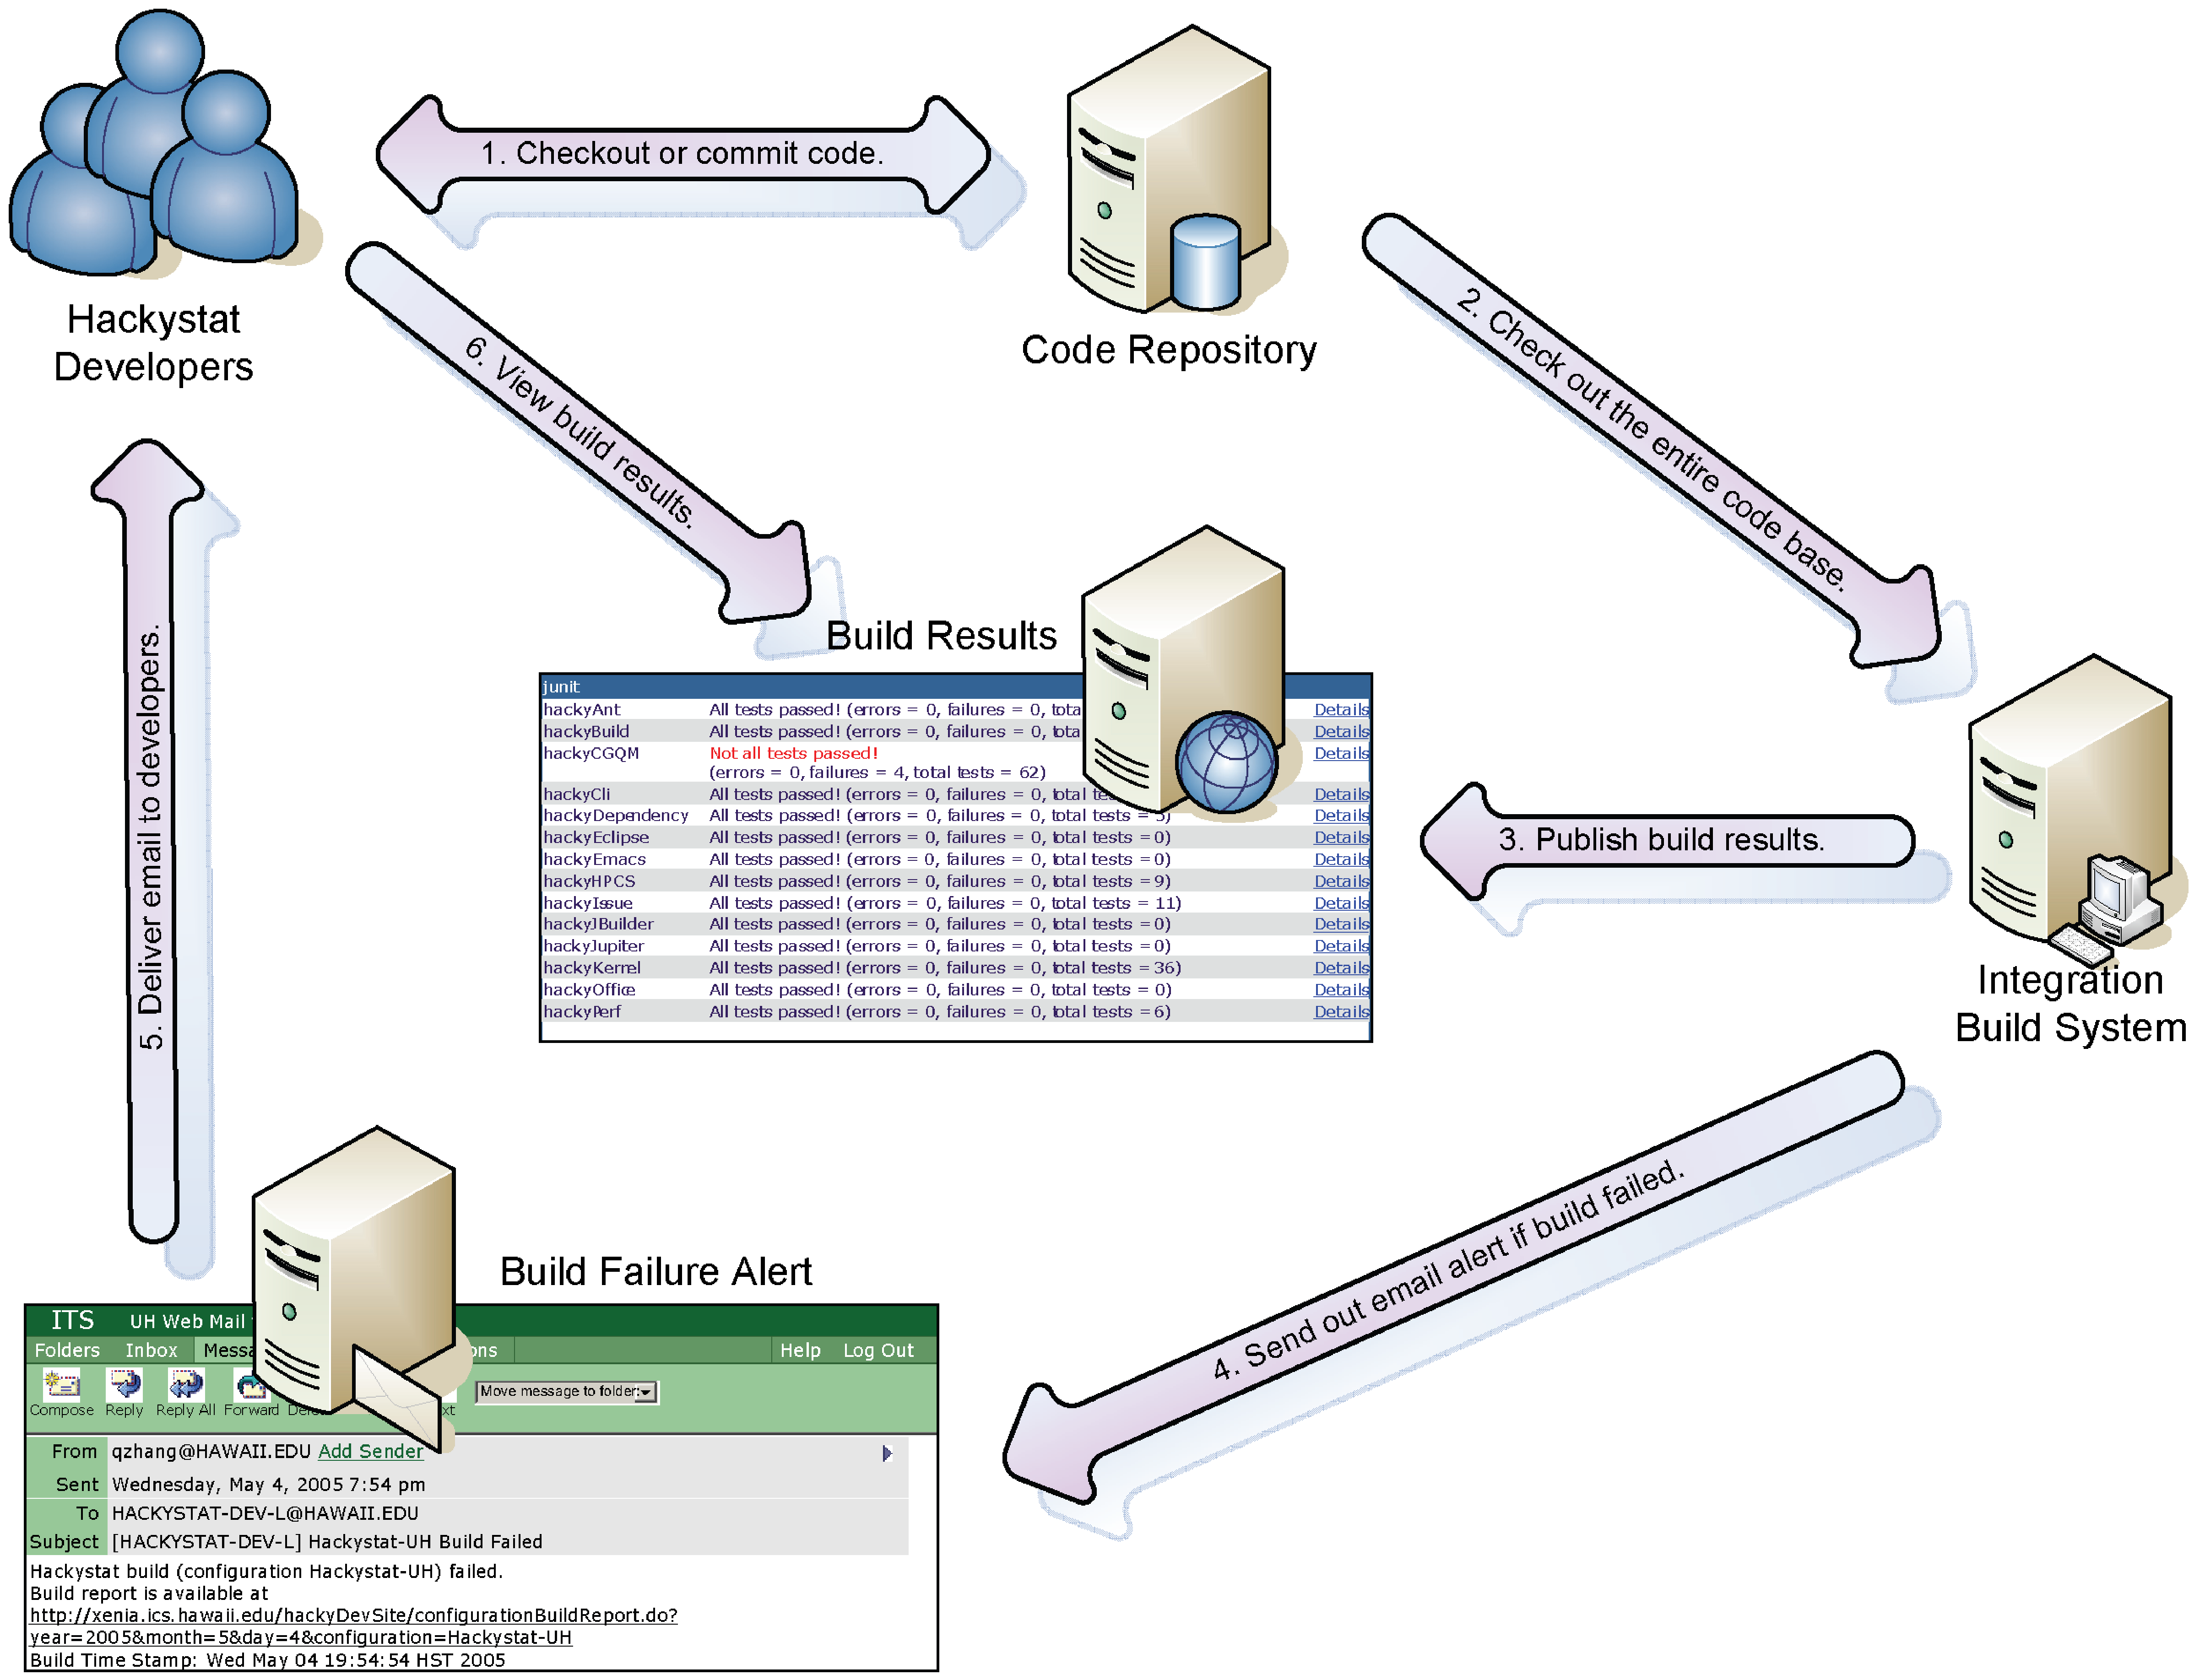
\includegraphics[width=1.00\textwidth]{figures/BuildProcess}
  \caption{CSDL Software Development Process}
  \label{fig:BuildProcess}
\end{figure}

Issues and project progress were tracked by an issue management system called \textit{Jira}. The lab had a status meeting every week. Code review was conducted as needed, but not on a regular basis. Though the team did not treat the software development as a strict \textit{timebox},\footnote{In software project management, a \textit{timebox} is a period of time in which to accomplish some task. The end date is set in stone and may not be changed. If necessary, less functionality than originally planned is provided on the release date.} it made regular releases about every three months.




%\subsection{Communicating Telemetry Analysis Results}

In order to increase the development team's awareness of software metrics, the CSDL development environment was instrumented with sensors to collect a variety of software product and process metrics. These metrics were sent to a server in CSDL for storage and analysis. I wrote a client-side application that automatically extracted telemetry charts from the server on a regular basis and displayed them on a 3x3 array of nine LCD monitors mounted on a wall inside the lab. Figure \ref{fig:TelemetryWall} is a picture of it. I call the nine-monitor wall the \textit{``telemetry wall,''} and the client-side application the \textit{``telemetry control center.''}

\begin{figure}[p]
  \center
  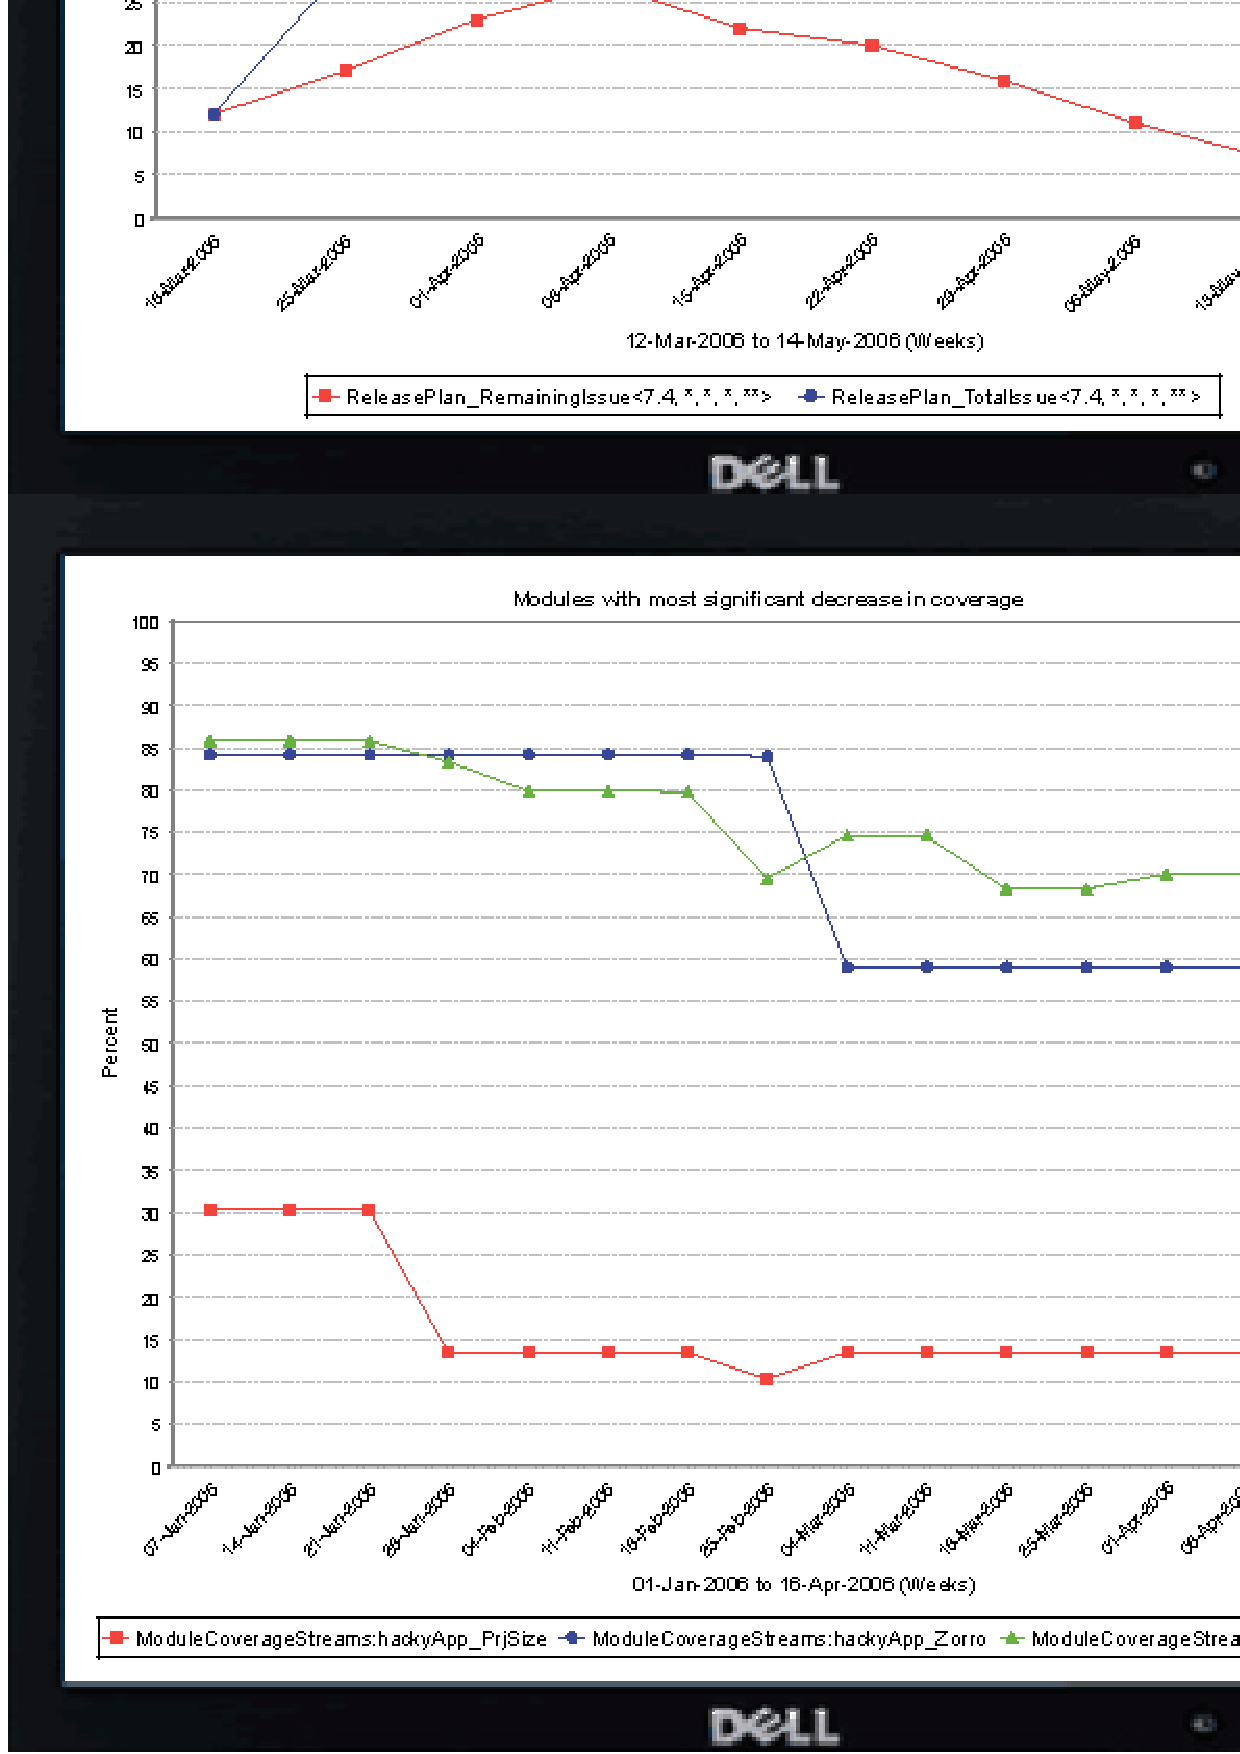
\includegraphics[width=1.00\textwidth]{figures/TelemetryWall}
  \caption{Telemetry Control Center on Telemetry Wall} 
  \label{fig:TelemetryWall}
\end{figure}

A configuration file provided the definitions of the telemetry charts to be displayed
using the standard telemetry language constructs (Section \ref{Telemetry:Component}). The telemetry control center retrieved the charts through the telemetry expert analysis interface (Figure \ref{fig:TelemetryExpertAnalysis}) provided by the software project telemetry implementation (Chapter  \ref{Chapter:Implementation}). The charts on the nine monitors formed a \textit{``telemetry scene.''} The telemetry control center application could be configured to cycle through different scenes automatically. 

The telemetry wall made a sequence of telemetry charts continuously available to the entire team automatically without any action on the part of the developers or the project manager. Rather than having to wait for a status update meeting, they could simply look at the telemetry wall to get a perspective on the current state of development. The development team had access to the regular telemetry analysis interface (Figure \ref{fig:TelemetryExpertAnalysis} and   \ref{fig:TelemetryReportChartStream}) through a web browser as well. However, the primary way I used to communicate telemetry analysis results to the team was the telemetry wall. It made it easy to discuss telemetry charts either formally in CSDL meetings or casually during lunch hours. 









%%%%%%%%%%%%%%%%%%%%%%%%%%%%%%%%%%%%%%%%%%%%%%%%%%%%%%%%%
%                                                       %
%                   S E C T I O N                       %
%                                                       %
%%%%%%%%%%%%%%%%%%%%%%%%%%%%%%%%%%%%%%%%%%%%%%%%%%%%%%%%%
\section{Researcher's Role}  \label{EvaluationInCSDL:Role}

My affiliation with CSDL started in 2003. I implemented the software project telemetry system as an extension to Hackystat. Dr. Philip Johnson is the director of CSDL. He is my dissertation adviser. He is also the project manager of Hackystat. I received a cornucopia of helpful advice from him during my implementation of software project telemetry.

During the period of this study, I acted as an on-site process expert introducing software project telemetry as a metrics-based process improvement program. I took careful observation of the team's development activity. I interviewed the team members and the project manager. I defined telemetry charts and made them available on the telemetry wall (Figure \ref{fig:TelemetryWall}). I discussed telemetry analysis results with the developers and the project manager. I recommended process changes. I helped the project manager institute changes to improve project management practices. I also helped the developers gain insights into their development processes.

At the same time, my own software development effort was concentrated on improving software project telemetry implementation based on the feedback received in this study. It included: (1) making sensors and telemetry charts available to meet the team's process-improvement and decision-making requirements, (2) enhancing the telemetry language to improve the display of telemetry charts, and (3) profiling and eliminating telemetry analysis runtime performance bottlenecks.









%%%%%%%%%%%%%%%%%%%%%%%%%%%%%%%%%%%%%%%%%%%%%%%%%%%%%%%%%
%                                                       %
%                   S E C T I O N                       %
%                                                       %
%%%%%%%%%%%%%%%%%%%%%%%%%%%%%%%%%%%%%%%%%%%%%%%%%%%%%%%%%
\section{Study Design}  \label{EvaluationInCSDL:StudyDesign}

%In the classroom study, I was able to gather insights from a relatively large number of people in a relatively short period of time. But the classroom study had limitations. The CSDL study was designed to have contrasting strengths and limitations. Unlike the classroom environment, there were a relatively small number of study participants in CSDL: five developers and one project manager. However, the project under development was much larger in scale. It contained nearly 300,000 lines of code in total, and had been underdevelopment for five years. The CSDL developers had significantly more software engineering experience and process maturity compared to the average student in the classroom.

The CSDL study was a mix-methods study to explore the use of software project telemetry in depth.
I have been affiliated with the lab for three years. Because of my familiarity with the CSDL software development environment and the small number of developers involved in the study, I was able to pursue a much more comprehensive data collection and analysis strategy over a much longer period of time compared to the classroom study. Instead of just giving the developers software project telemetry tools and observing how they used them, I took a more active role by acting as a process expert. I introduced software project telemetry as a metrics-based process improvement program. I proposed improvements to the CSDL software development process, and helped the project manager institute the changes. The steps I took consisted of the following iterative steps: %(Figure\ref{fig:CsdlStudyMethod}):

\begin{enumerate}
  \setlength{\itemsep}{0pt}
  \setlength{\parskip}{0pt}
	\item Collect data from observations and interviews.
	\item Code the data in order to generate hypotheses.
  \item Propose improvements to the CSDL software development process.
  \item Continue to collect data to assess the effectiveness of the changes.
  \item Draw conclusions from the data gathered.
\end{enumerate}
  
%\begin{figure}[p]
%  \center
%  \includegraphics[height=0.80\textheight]{figures/CsdlStudyMethod}
%  \caption{CSDL Research Strategy} 
%  \label{fig:CsdlStudyMethod}
%\end{figure}

The study involved many elements from the constructivist paradigm. It was a case study in which I explored the use of software project telemetry in CSDL extensively. I collected data from observations and interviews, and generated hypotheses from the data. My observation strategy was complete involvement as a full participant instead of an outside spectator. I was in the lab almost every day working with the developers, and attended every weekly status update meeting. My interview strategy was in-depth interview instead of structured interview. Both formal and informal interviews were used. I always encouraged free responses. The purpose was to gather much richer data about how the developers and the project manager interacted with software project telemetry to make decisions. I have to admit that my affiliation with CSDL was a source of bias. Years of affiliation might have ingrained in me the software process practiced in CSDL, and thus made me unable to see important information in my observations and interviews. However, the bias was mitigated through several factors. My observation was much less disruptive to the developers than having a stranger watching over their backs. My detailed knowledge about the project under development made it easy for me to link the observed facts to the contextual information in CSDL, so that I could have much deeper insights into ``what's going on'' than an outsider. I often reconciled my interpretation of observed facts with the developers and the project manager in interviews.

The study also involved an element from the post-positivist paradigm. After the hypotheses were generated, I tested them in a limited way by making changes to the telemetry system or implementing new facilities to see if the hypothesized outcome would come true. 
To some extent, this hypothesis testing procedure could be viewed as the simplest and uncontrolled form of experiment. The difference is that most experiments rely on statistical analysis to draw conclusions, but mine does not.


 






%%%%%%%%%%%%%%%%%%%%%%%%%%%%%%%%%%%%%%%%%%%%%%%%%%%%%%%%%
%                                                       %
%                   S E C T I O N                       %
%                                                       %
%%%%%%%%%%%%%%%%%%%%%%%%%%%%%%%%%%%%%%%%%%%%%%%%%%%%%%%%%
\section{Data Collection and Analysis} \label{EvaluationInCSDL:DataCollectionAnalysis}

My data came from both observations and interviews. The observations included almost everything related to CSDL software development. The interviews covered a variety of topics, from the discussion of the current development process and telemetry analysis results, to the exploration of improvement options and assessment of change impact.

The data were stored and organized using a software program called \textit{``Confluence.''} The reason that I used the software was because of the ease with which different types of documents could be organized and accessed anywhere through a web interface. Though Confluence is mainly designed for knowledge sharing, I did not share my field notes with the study participants. I divided the \textit{Confluence} data storage area into two sections: ``Raw Data'' and ``Hypotheses.'' At the end of the study, I had accumulated a total of 173 entries in the ``Raw Data'' section, and generated a total of 9 findings in the ``Hypotheses'' section.

\begin{itemize}
	\item \textbf{Raw Data} --- They were field notes from observations and informal interviews, and transcripts from formal interviews. The data in this category were further organized into two levels. Second level entries were immediate follow-up observations and interviews closely related to their parent entry in the first level. The total 173 entries in this section consisted of 109 first level entries and 64 second level entries. Figure \ref{fig:CSDL-RawData1} shows an index page with links to all raw data entries, while Figure \ref{fig:CSDL-RawData2} shows the details of one of the entries. The raw data themselves cannot be published because of privacy issues. However, I included a summary for each first level entry in Appendix \ref{Appendix:DataInCSDL}. The summaries were assigned unique identification numbers, which were referenced in my discussion of the study results in Section \ref{EvaluationInCSDL:EventsDescription}. The intention is to provide the reader a mechanism to ``audit'' my conclusions in some sense.

  \item \textbf{Hypotheses} --- They were hypotheses regarding the use of software project telemetry from my conceptualized ideas based on the raw data. All entries in this section were formatted into five subsections: (1) pre-hypothesis links to raw data entries, (2) generated hypothesis, (3) change implementation, (4) post-hypothesis links to raw data entries, and (5) conclusion. Figure \ref{fig:CSDL-Hypothesis1} is an index page with links to all generated hypotheses, while Figure \ref{fig:CSDL-Hypothesis2} shows the details of one of the hypotheses. The details of each finding were reported in Section \ref{EvaluationInCSDL:EventsDescription}.

\end{itemize}


The approach I followed to generate hypotheses from the data was inspired by grounded theory. 
As soon as the field notes and interview transcripts were entered into the raw data section, I applied \textit{``open coding''} to label the text with different category names (i.e., \textit{``conceptualization''} of ``what's going on'' in grounded theory terminology). The coding was done as annotations to the raw data text (Figure   \ref{fig:CSDL-RawData2}), and was stored together with the raw data entry. I constantly compared, modified, and merged the category names when new data came in. During the process of \textit{open coding}, some themes (i.e., \textit{``core variables''}) emerged naturally. They were related to the use of software project telemetry. I continued to collect and categorize data after the emergence of the themes. However, at this step, my data collection was more selective. I paid more attention to those related to the identified themes (i.e., \textit{``selective coding''}).
The next step was \textit{``theoretical memoing''}, in which I generated my hypotheses, such as the best practice of software project telemetry, the plausible reason for the problems encountered during its use, and the possible remedy to improve the system. The hypotheses were entered in the ``hypotheses'' section in the Confluence data store, together with the links to the relevant raw data entries. I did not have a separate \textit{``sorting''} step. The links to the relevant raw data in each hypothesis entry served the same purpose as sorting.
In contrast to grounded theory where hypotheses are the end goal, my data collection and analysis did not stop there. After the hypotheses were generated, I made changes to the telemetry system, implemented new facilities, and collected additional data in an attempt to confirm or refine the hypotheses. The additional data were recorded in the ``raw data'' section as well, and any refinement to the previously generated hypotheses was also noted in the ``hypotheses'' section.


\begin{figure}[p]
  \center
  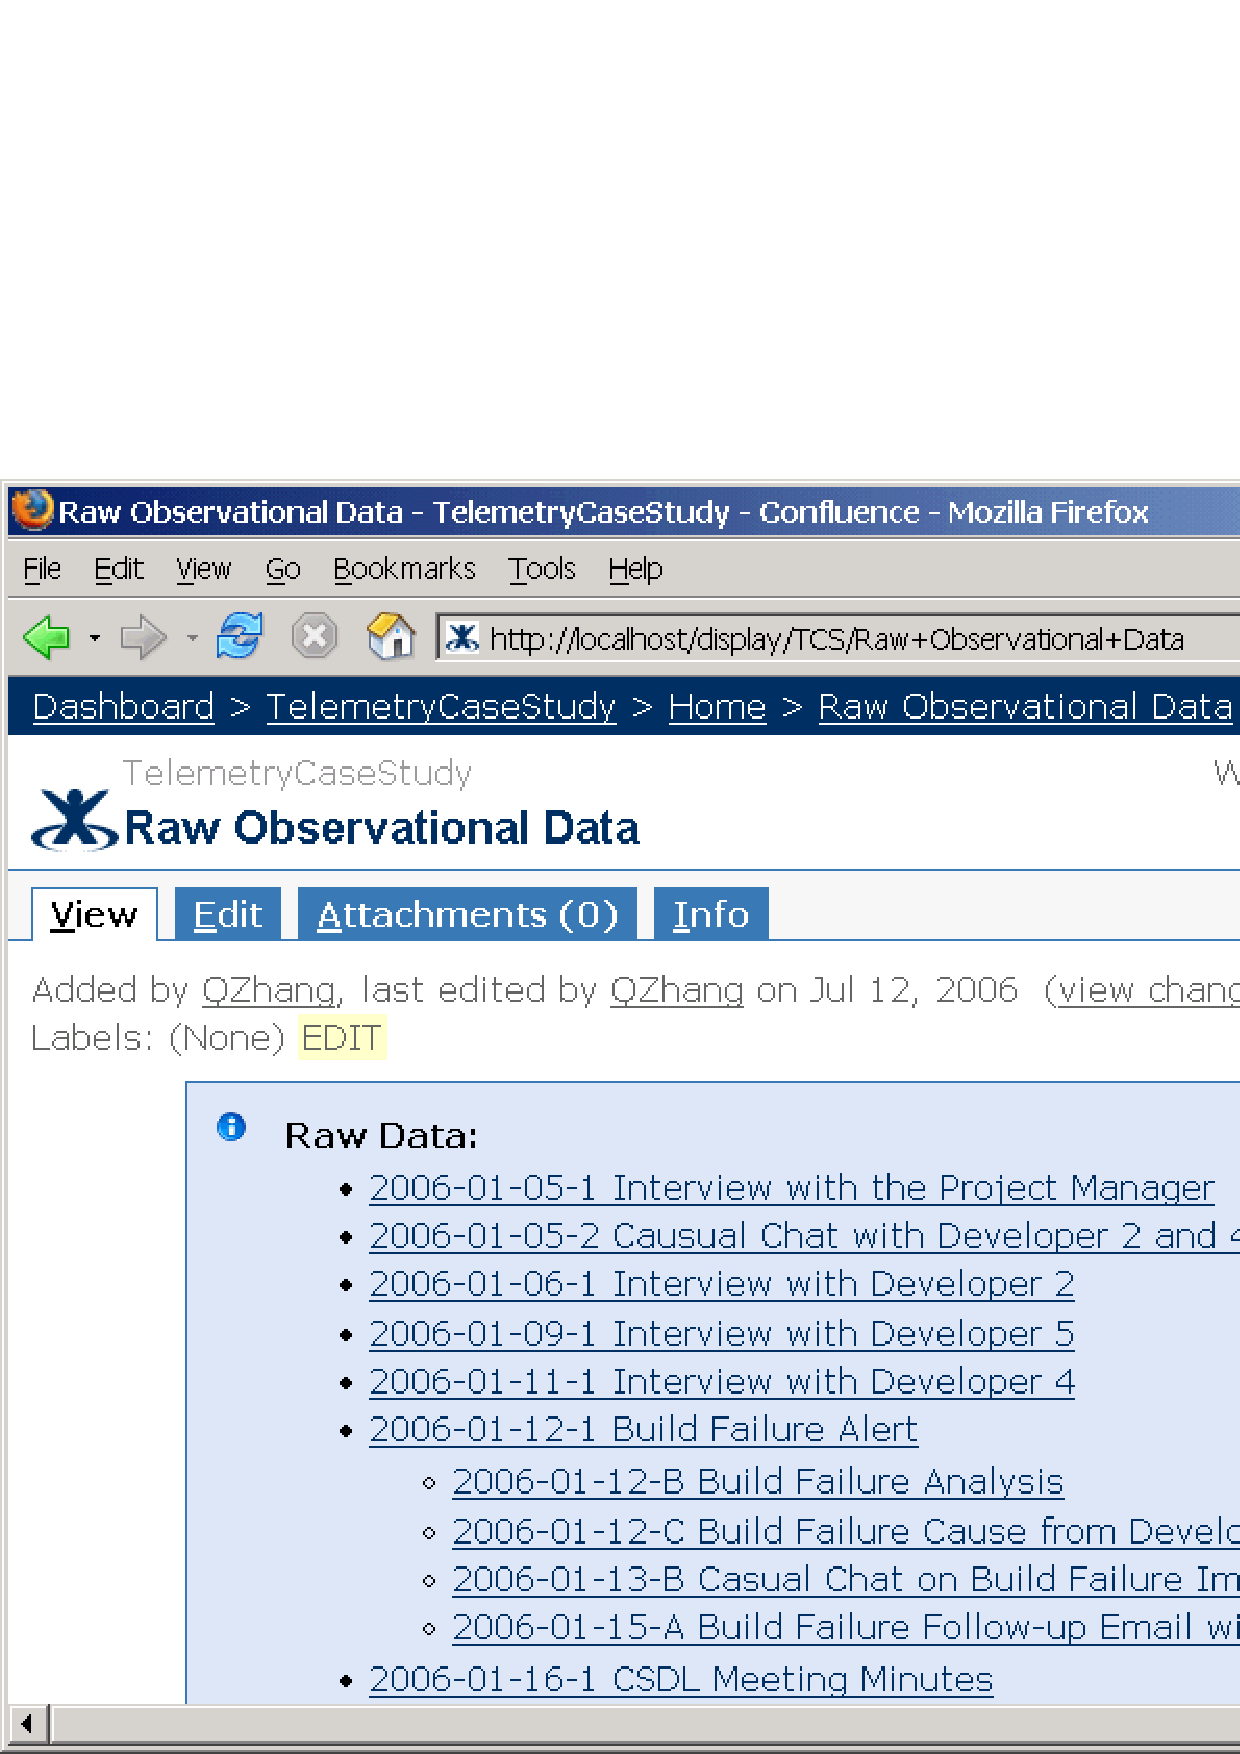
\includegraphics[width=1.00\textwidth]{figures/CSDL-RawData1}
  \caption{A Page with Links to all Raw Data Entries} 
  \label{fig:CSDL-RawData1}
\end{figure}
	
\begin{figure}[p]
  \center
  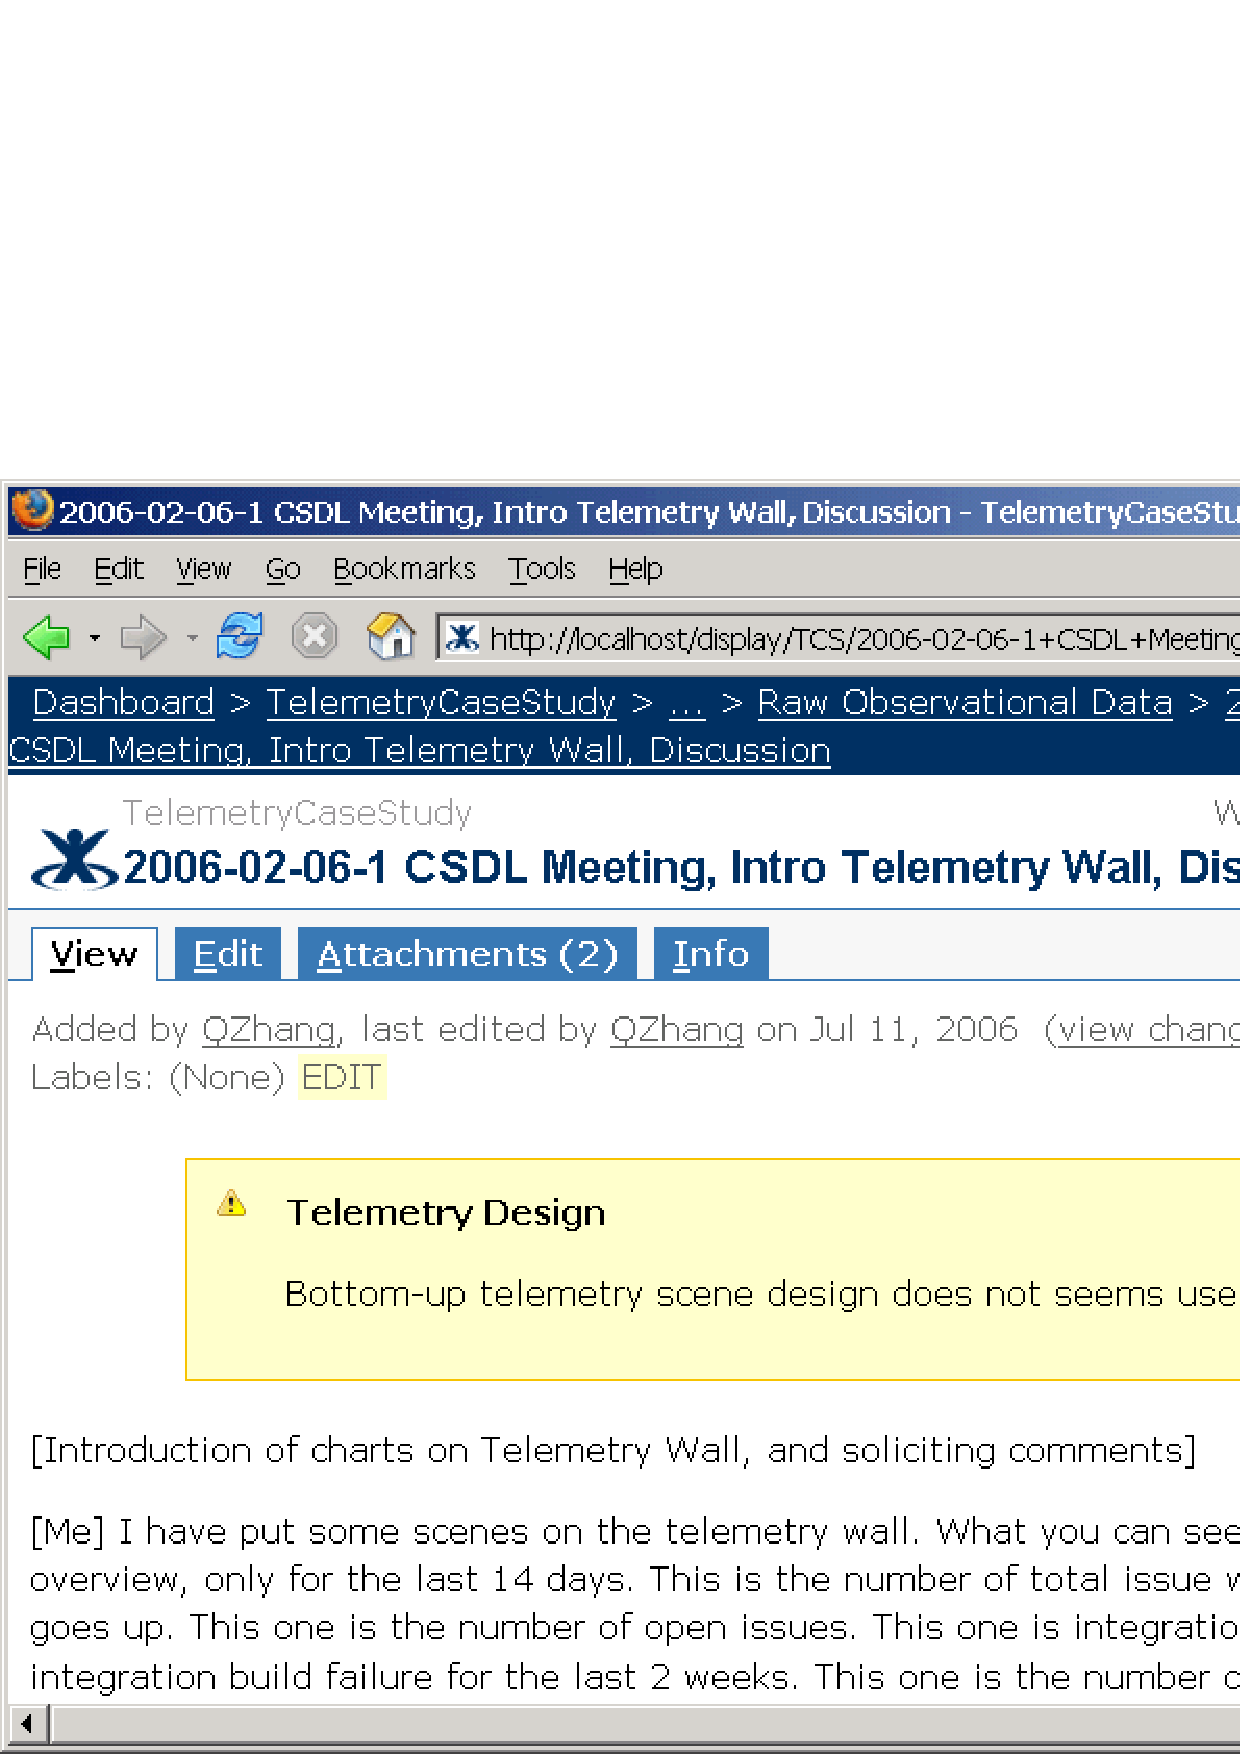
\includegraphics[width=1.00\textwidth]{figures/CSDL-RawData2}
  \caption{One of the Raw Data Entries with Annotation} 
  \label{fig:CSDL-RawData2}
\end{figure}	
	

\begin{figure}[p]
  \center
  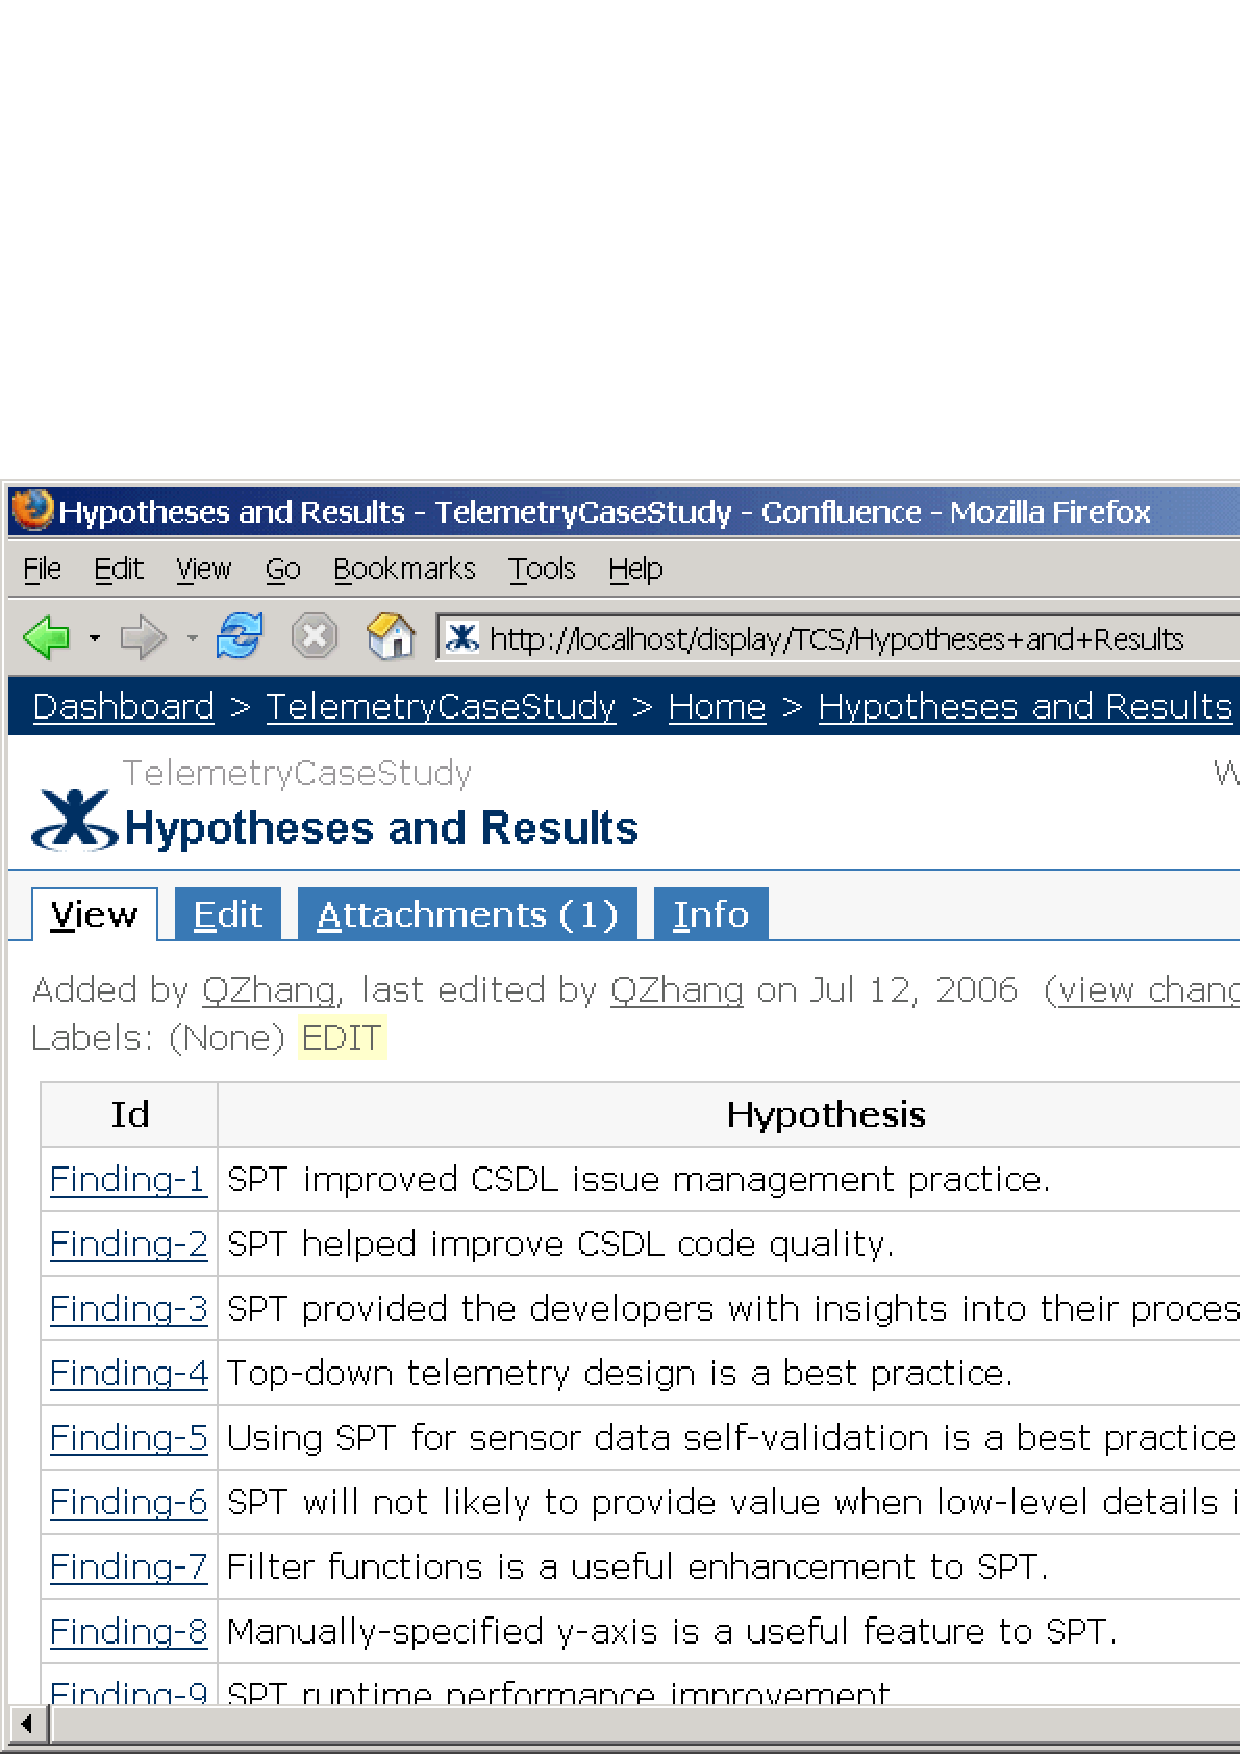
\includegraphics[width=1.00\textwidth]{figures/CSDL-Hypothesis1}
  \caption{A Tables with Links to all Generated Hypotheses} 
  \label{fig:CSDL-Hypothesis1}
\end{figure}

\begin{figure}[p]
  \center
  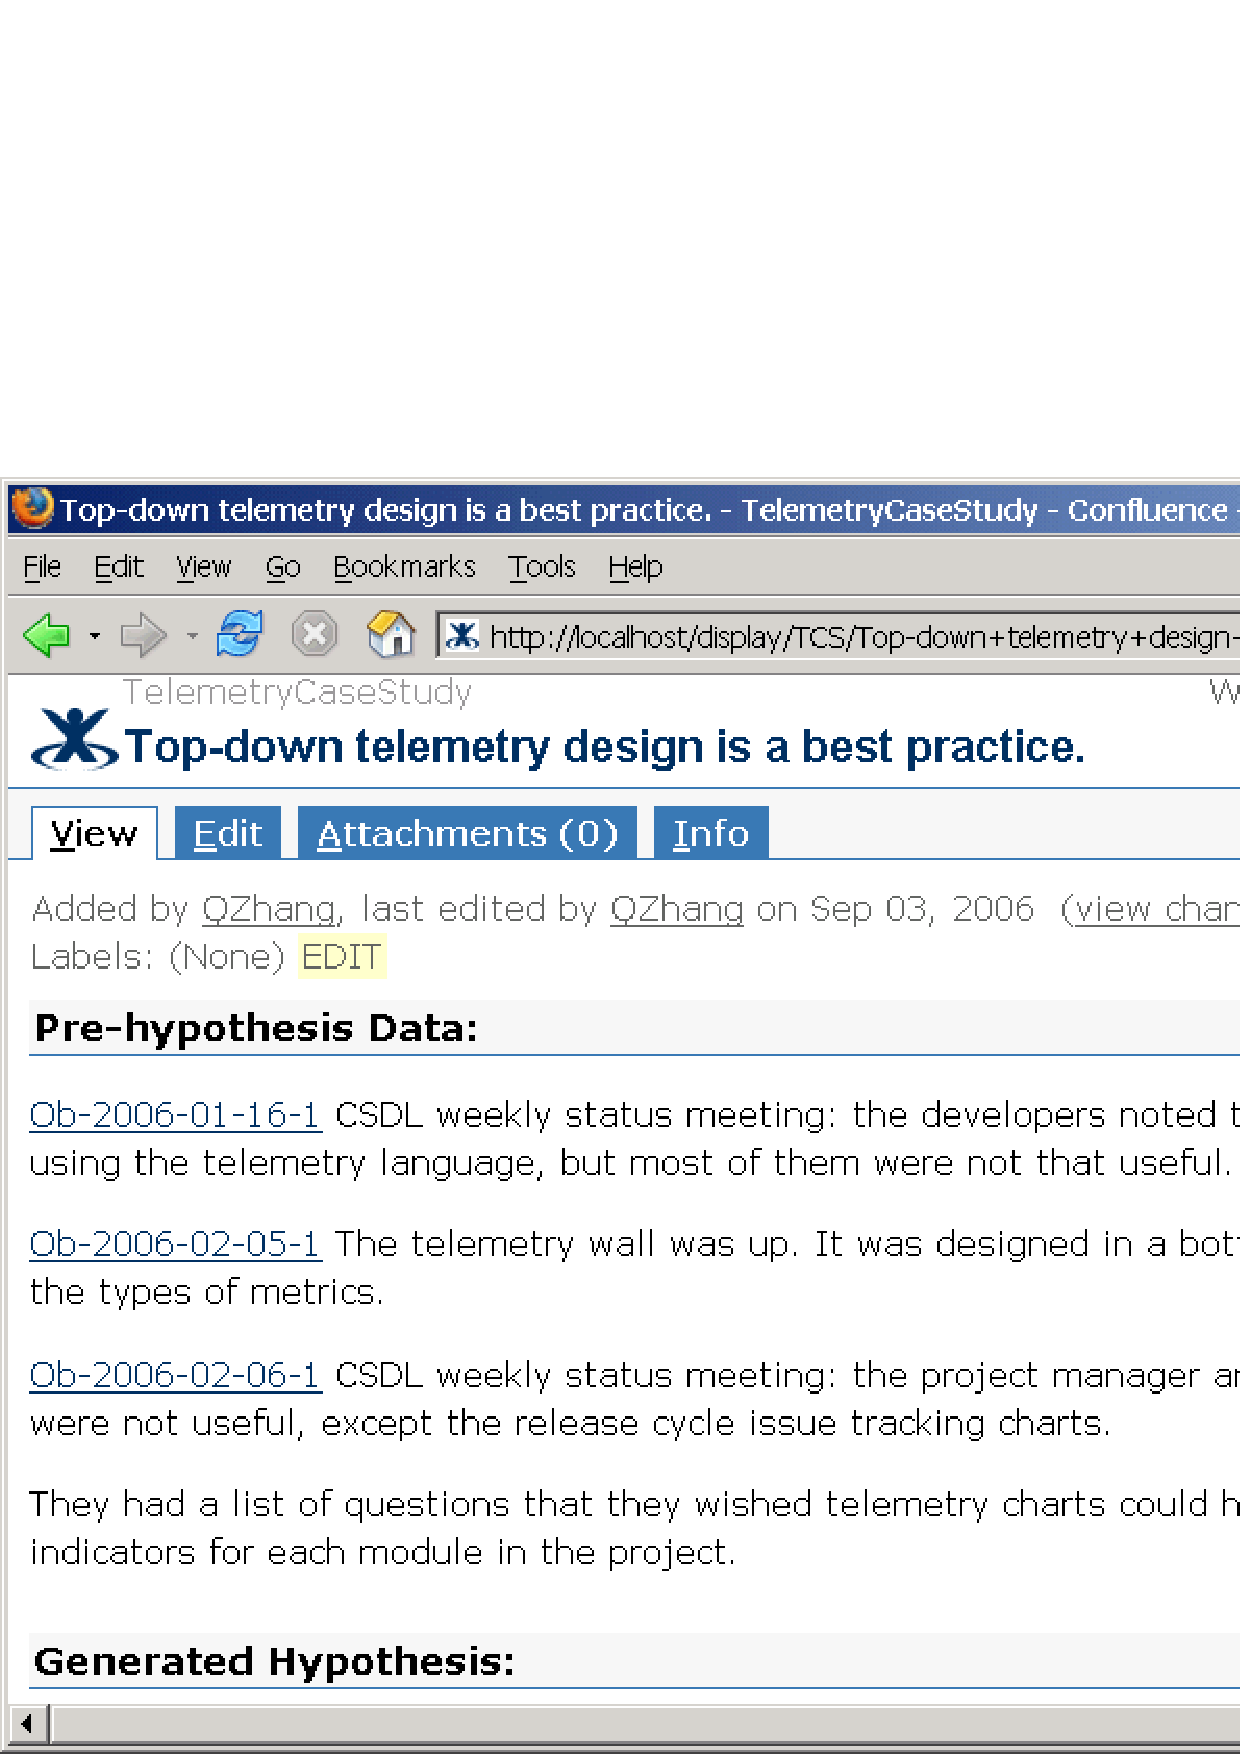
\includegraphics[width=1.00\textwidth]{figures/CSDL-Hypothesis2}
  \caption{One of the Generated Hypotheses} 
  \label{fig:CSDL-Hypothesis2}
\end{figure}








%%%%%%%% Sub Section %%%%%%%%%
%\clearpage
%\subsection{Quantitative Data}
%
%\textcolor{red}{To be removed}
%
%Quantitative data were collected from software product and process metrics.
%The CSDL development environment was heavily instrumented. In order to collect software process metrics, sensors were attached to the IDEs on the developers' workstations, to the SVN source code repository, to the Jira issue management system, and to the nightly integration build system. In order to collect software product metrics, a set of code analyzers were invoked automatically on software artifacts every night. 
%
%Sensors were everywhere. The metrics collection practice in CSDL was to collect whatever metrics possible regardless of whether you could think of a use for such metrics or not. The rationale behind the practice was the low cost associated with the sensor-based metrics collection mechanism. In addition, by using as many sensors as possible, the lab was able to assess and improve the quality of the sensors and also determine how the server behaved under load. All the sensors send metrics to a server located inside CSDL. The metrics were used as input for telemetry analysis.
%
%\begin{figure}[p]
%  \center
%  \includegraphics[width=1.00\textwidth]{figures/CSDL-QuantitativeData1}
%  \caption{\textcolor{red}{TO BE UPDATED:} CSDL Study Quantitative Data Overview} 
%  \label{fig:CSDL-QuantitativeData1}
%\end{figure}
%
%\begin{figure}[p]
%  \center
%  \includegraphics[width=1.00\textwidth]{figures/CSDL-QuantitativeData2}
%  \caption{\textcolor{red}{TO BE UPDATED:} CSDL Study Quantitative Data Drilldown} 
%  \label{fig:CSDL-QuantitativeData2}
%\end{figure}







%%%%%%%%%%%%%%%%%%%%%%%%%%%%%%%%%%%%%%%%%%%%%%%%%%%%%%%%%
%                                                       %
%                   S E C T I O N                       %
%                                                       %
%%%%%%%%%%%%%%%%%%%%%%%%%%%%%%%%%%%%%%%%%%%%%%%%%%%%%%%%%

\section{Results} \label{EvaluationInCSDL:EventsDescription}

The results of the study are the findings regarding the use of software project telemetry. Each finding is reported in its own sub-section, which is organized into the following parts:

\begin{itemize}
	\item \textbf{Pre-hypothesis Data}\footnote{To preserve privacy, I used the word \textit{``he''} when referring to individual developer throughout my report, even though there were both male and female participants in the study.} --- Summary information about the data I collected that led to the generated hypothesis.

	\item \textbf{Generated Hypothesis} --- The hypothesis, such as the best practice of software project telemetry, the plausible reasons for the problems encountered during its use, and the possible remedies to improve the system.
	
	\item \textbf{Intervention} --- The changes I introduced based on the hypothesis in order to use software project telemetry more effectively, or overcome the problems encountered during its use.
	
	\item \textbf{Post-hypothesis Data}\footnote{Same as above.} --- The additional data I collected after the changes were implemented, which were used to confirm or refine the generated hypothesis. 
	
	\item \textbf{Conclusion} --- The final finding and comments.
	
\end{itemize}
	
Finally, at the end of each report, I included an ``elaboration'' to provide much more detailed account of the finding.

%This section reports on several experiences from applying \textit{software project telemetry} in CSDL as a metrics-based process improvement program. Some experiences were successful. Some were not. Both types are reported in this section, and conclusions were drawn in the next section (Section \ref{EvaluationInCSDL:StudyConclusion}).






%%%%%%%%%%%%%%%
%  S T O R Y  %
%%%%%%%%%%%%%%%
\clearpage
%\subsection{Software project telemetry improved CSDL issue management practice.}
\subsection{Improvement on CSDL Release Cycle Issue Management}
\label{EvaluationInCSDL:EventsDescription:ProjectIssueTracking}

\subsubsection{Pre-hypothesis Data:}
\begin{itemize}
  \setlength{\itemsep}{0pt}
  \setlength{\parskip}{0pt}
  \item 2006-01-05-1: I discussed the existing analysis of issue metrics with the project manager in an interview. He did not utilize the metrics in project management, because the analysis was inadequate for release cycle planning and tracking. 
	\item 2006-01-05-2: I interviewed two developers on their opinions about the utility of the metrics currently collected in the lab. One of them thought the issue related metrics were not that useful, because they were quite different from what he had anticipated. 
	\item 2006-01-06-1: I discussed the current status of issue management with a developer, who told me that most of his development activities were not recorded in the issue database.
	\item 2006-01-09-1: I held a discussion with another developer, who estimated that only 20\% - 30\% of his development activities were tracked by the issue database. He also told me that he never followed the issue priority in resolving issues assigned to him.
	\item 2006-01-11-1: I held a discussion with yet another developer, who estimated that less than 15\% of his development activities were tracked by the issue database. He told me that most of his issues were assigned through emails instead of the issue management system. He also told me that he did not understand how issue metrics were computed.
\end{itemize}
	
\subsubsection{Generated Hypothesis:}
There were two reasons why the issue metrics were not useful: (1) the issue tracking system severely under-represented the actual development effort; and (2) the issues scheduled for a release did not reflect the actual items that the team wanted to accomplish in that release cycle. If these two problems could be resolved, then the issue tracking telemetry charts could be used not only to track the progress in a release cycle, but also to make in-process predictions about the release schedule. 

\subsubsection{Intervention:}
I identified the problem to the project manager and the developers, and explored options with them to make the issue tracking database more consistent with the actual development effort.

\subsubsection{Post-hypothesis Data:}
\begin{itemize}
  \setlength{\itemsep}{0pt}
  \setlength{\parskip}{0pt}
	\item 2006-01-16-1: The project manager discussed possible changes to improve the issue management practice with the developers in a weekly status meeting.
	\item 2006-01-19-2: As part of corrective measures, the project manager went through all issues and tagged them with realistic fix version numbers to get ready for the new release cycle (i.e., Release 7.3).
	\item 2006-01-19-3: As part of corrective measures, the project manager sent out an email requiring that all future commits should have issue Id in commit log comment field.
	\item 2006-01-23-2: This was the first time in my observation that the new issues assigned in the weekly status meeting were recorded in the issue management system.
	\item 2006-01-29-1: I enhanced the Jira sensor to collect missing information required for issue tracking telemetry analyses.
	\item 2006-02-03-1: I made the issue tracking charts available on the telemetry wall, and showed them to a developer. He commented that they could be used not only to track issue status but also to predict system release date.
	\item 2006-02-06-1: The project issue tracking charts were formally introduced in a CSDL meeting. The project manager commented that they were ``highly useful.''
  \item 2006-03-13-1: I interviewed a developer. He confirmed that almost all his work was tracked by the issue tracking system now.  
  \item 2006-03-15-2: I interviewed two more developers. They all confirmed that most of their work was tracked by the issue tracking system.
	\item 2006-03-20-2: The project manager reviewed the issue tracking chart after release 7.3 was finished, and reflected that the chart helped him determine whether more issues could be added to that release. 
  \item 2006-04-07-3: The project manager was comparing release 7.4 issue tracking chart with the chart from the previous release cycle to make short term predictions.
  \item 2006-04-26-1: During an interview, the project manager told me that his project management skill had improved a lot with respect to release cycle issue tracking and planning.
\end{itemize}

\subsubsection{Conclusion:}
The additional data appears to confirm the hypothesis. The corrective measures were simple but effective. The issue tracking charts were found useful by the project manager for release cycle progress tracking and in-process prediction.

\subsubsection{Elaboration:}

CSDL used an issue management tool called \textit{``Jira''} to record and track issues related to the \textit{Hackystat} development. The types of the issues managed by \textit{Jira} included feature requests, task assignments, and software bugs. CSDL had been using \textit{Jira} and collecting issue related metrics for almost two years.
During an interview at the beginning of this study, the project manager revealed that he did not utilize the issue metrics to plan and track issues in a release cycle. I also interviewed the developers asking them their opinions about the metrics being collected in CSDL. One of them identified the issue metrics as one of not-so-useful metrics. Two problems were identified in the discussions, both related to the way issues were managed and tracked:

\begin{itemize}
  \item The issue management system significantly under-represented the actual development effort. For example, the percentage of issues tracked by \textit{Jira} was less than 15\% according to one developer. Another developer estimated this number between 20\% to 30\%. A lot of issues were assigned in emails or weekly status meetings, instead of through the issue management system.
  
	\item The open issues in the issue management system did not correspond to the expectation for the set of items to be accomplished in a release cycle. I raised this problem in an interview with the project manager. In his own words, when preparing for a stable release, he simply \textit{``chucked the remaining unresolved issues over the fence into the next version.''}
\end{itemize}

My hypothesis was that the issue metrics were not useful precisely because of the two problems identified above. If the issue tracking database could be made consistent with the actual development effort, then the issue telemetry charts could be used not only to track the progress in a release cycle, but also to make in-process predictions about the release schedule.

After I identified the problems to the project manager and the developers, they took corrective measures quickly. On the manager side, the project manager went over all the issues, prioritized them, and tagged them with realistic fix version numbers. On the developer side,	the developers were required to supply a log message referencing an issue number whenever making a commit. The idea was that the practice would remind them to create a \textit{Jira} issue if it had not already existed.

The result of these changes was both effective and positive, because they made it possible to generate issue tracking charts that reflected the actual development activities. For example, Figure \ref{fig:CSDL-Issue730} and \ref{fig:CSDL-IssueActiveTime730} were taken from the Hackystat release cycle 7.3, which lasted from mid-January to mid-March.

Figure \ref{fig:CSDL-Issue730} is a telemetry chart showing the number of total \textit{vs.} remaining issues on the last day of each week during the Hackystat 7.3 release cycle. The blue line on the top is the total number of issues scheduled for that release, while the red line below is the number of remaining issues. The telemetry chart clearly indicates that CSDL did not schedule everything up-front but rather added new issues almost every week. There was a concern that adding new issues constantly might lead to unmanageable release cycles. However, the project manager told me that he used the trend about issue closure in the red line to control whether or not more issues could be added to the release cycle. As the chart indicates, after initial weeks of issue build-up, CSDL was able to make consistent progress toward zero open issue and the delivery of the 7.3 stable release.

Figure \ref{fig:CSDL-IssueActiveTime730} is a telemetry chart showing the cumulative number of closed issues \textit{vs.} the cumulative amount of developer \textit{``active time''} on a weekly basis during the Hackystat 7.3 release cycle. Though the active time required for an individual issue varied significantly with the actual issue in question, over time these differences appeared to \textit{``smooth out.''} The chart indicates that for the 7.3 release cycle, CSDL issue closure rate was pretty constant (around 12 issues per week, or 3 active time hours per issue). The near linear relationship is quite provocative: if this same relationship holds true for future releases, then it provides strong evidence for a predictive relationship and a basis for cost and schedule estimation.

Figure \ref{fig:CSDL-Issue740} and \ref{fig:CSDL-IssueActiveTime740} were taken from the Hackystat release cycle 7.4. The telemetry exhibited similar trends as those in the release cycle 7.3. A revealing observation was that in the middle of the release cycle 7.4, the project manager was constantly comparing telemetry shapes between 7.3 and 7.4 releases and making in-process schedule predictions about 7.4 release date. These charts not only allowed CSDL to track progress of each release cycle, but also established a baseline for planning and scheduling of future releases.

\begin{figure}[p]
  \center
  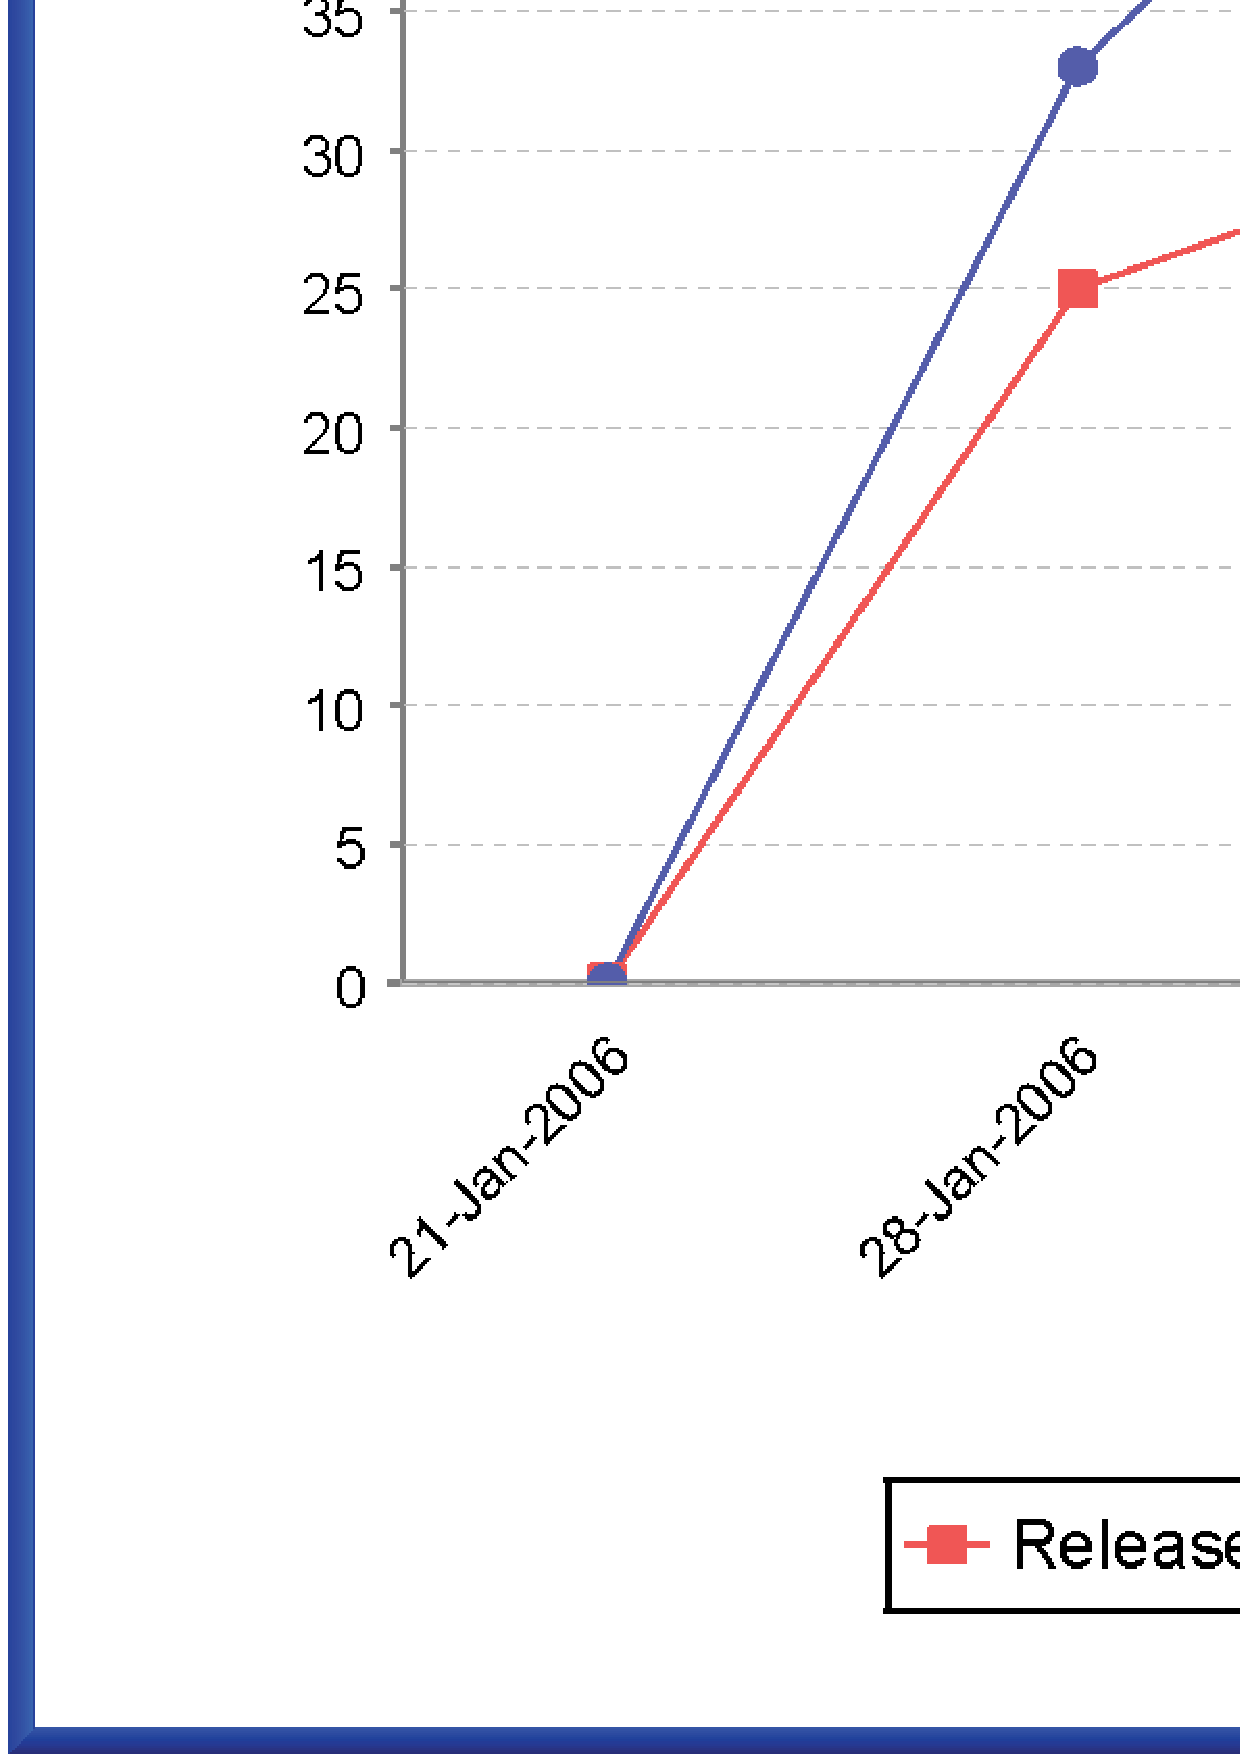
\includegraphics[width=0.70\textwidth]{figures/CSDL-Issue730}
  \caption{Hackystat Release Cycle 7.3 --- Total Issues vs. Remaining Issues} 
  \label{fig:CSDL-Issue730}
\end{figure}

\begin{figure}[p]
  \center
  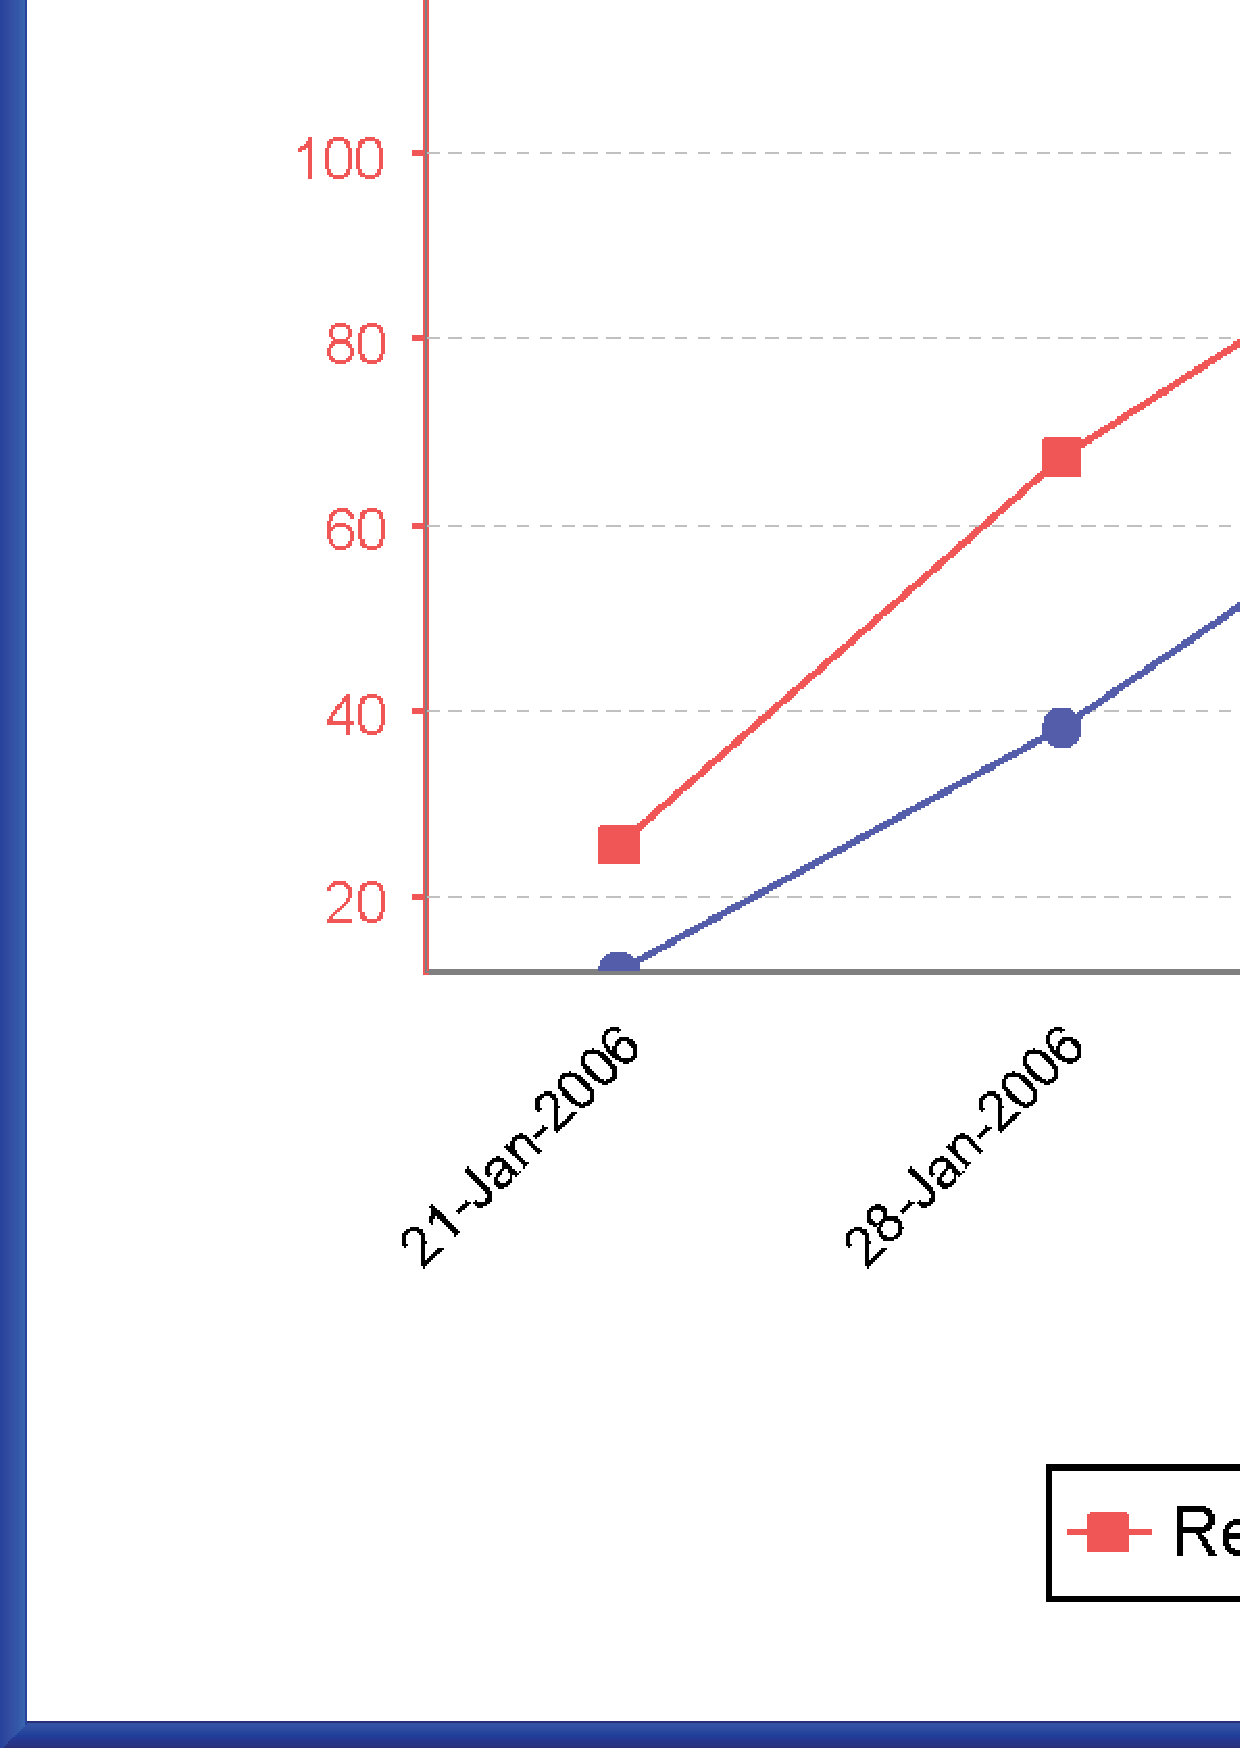
\includegraphics[width=0.70\textwidth]{figures/CSDL-IssueActiveTime730}
  \caption{Hackystat Release Cycle 7.3 --- Total Issues vs. Active Time} 
  \label{fig:CSDL-IssueActiveTime730}
\end{figure}


\begin{figure}[p]
  \center
  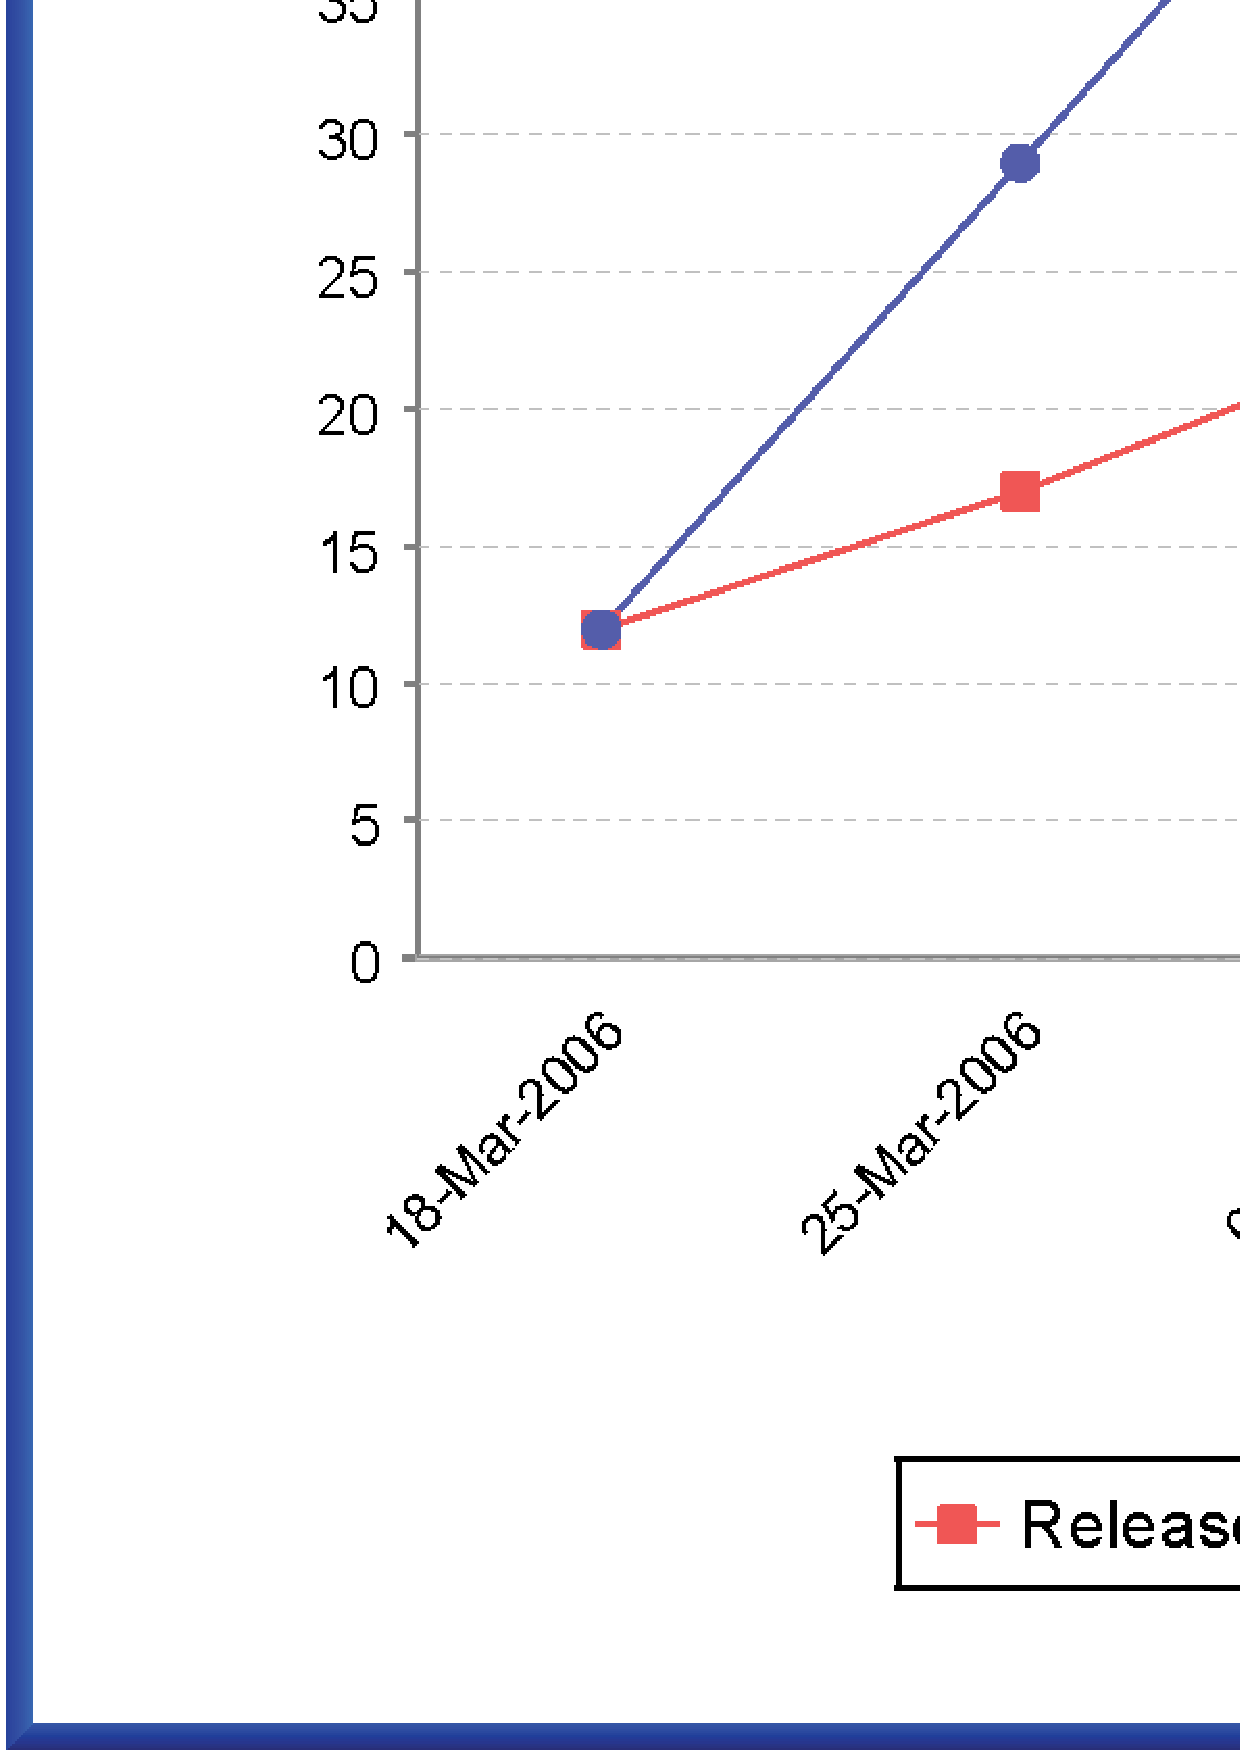
\includegraphics[width=0.70\textwidth]{figures/CSDL-Issue740}
  \caption{Hackystat Release Cycle 7.4 --- Total Issues vs. Remaining Issues} 
  \label{fig:CSDL-Issue740}
\end{figure}

\begin{figure}[p]
  \center
  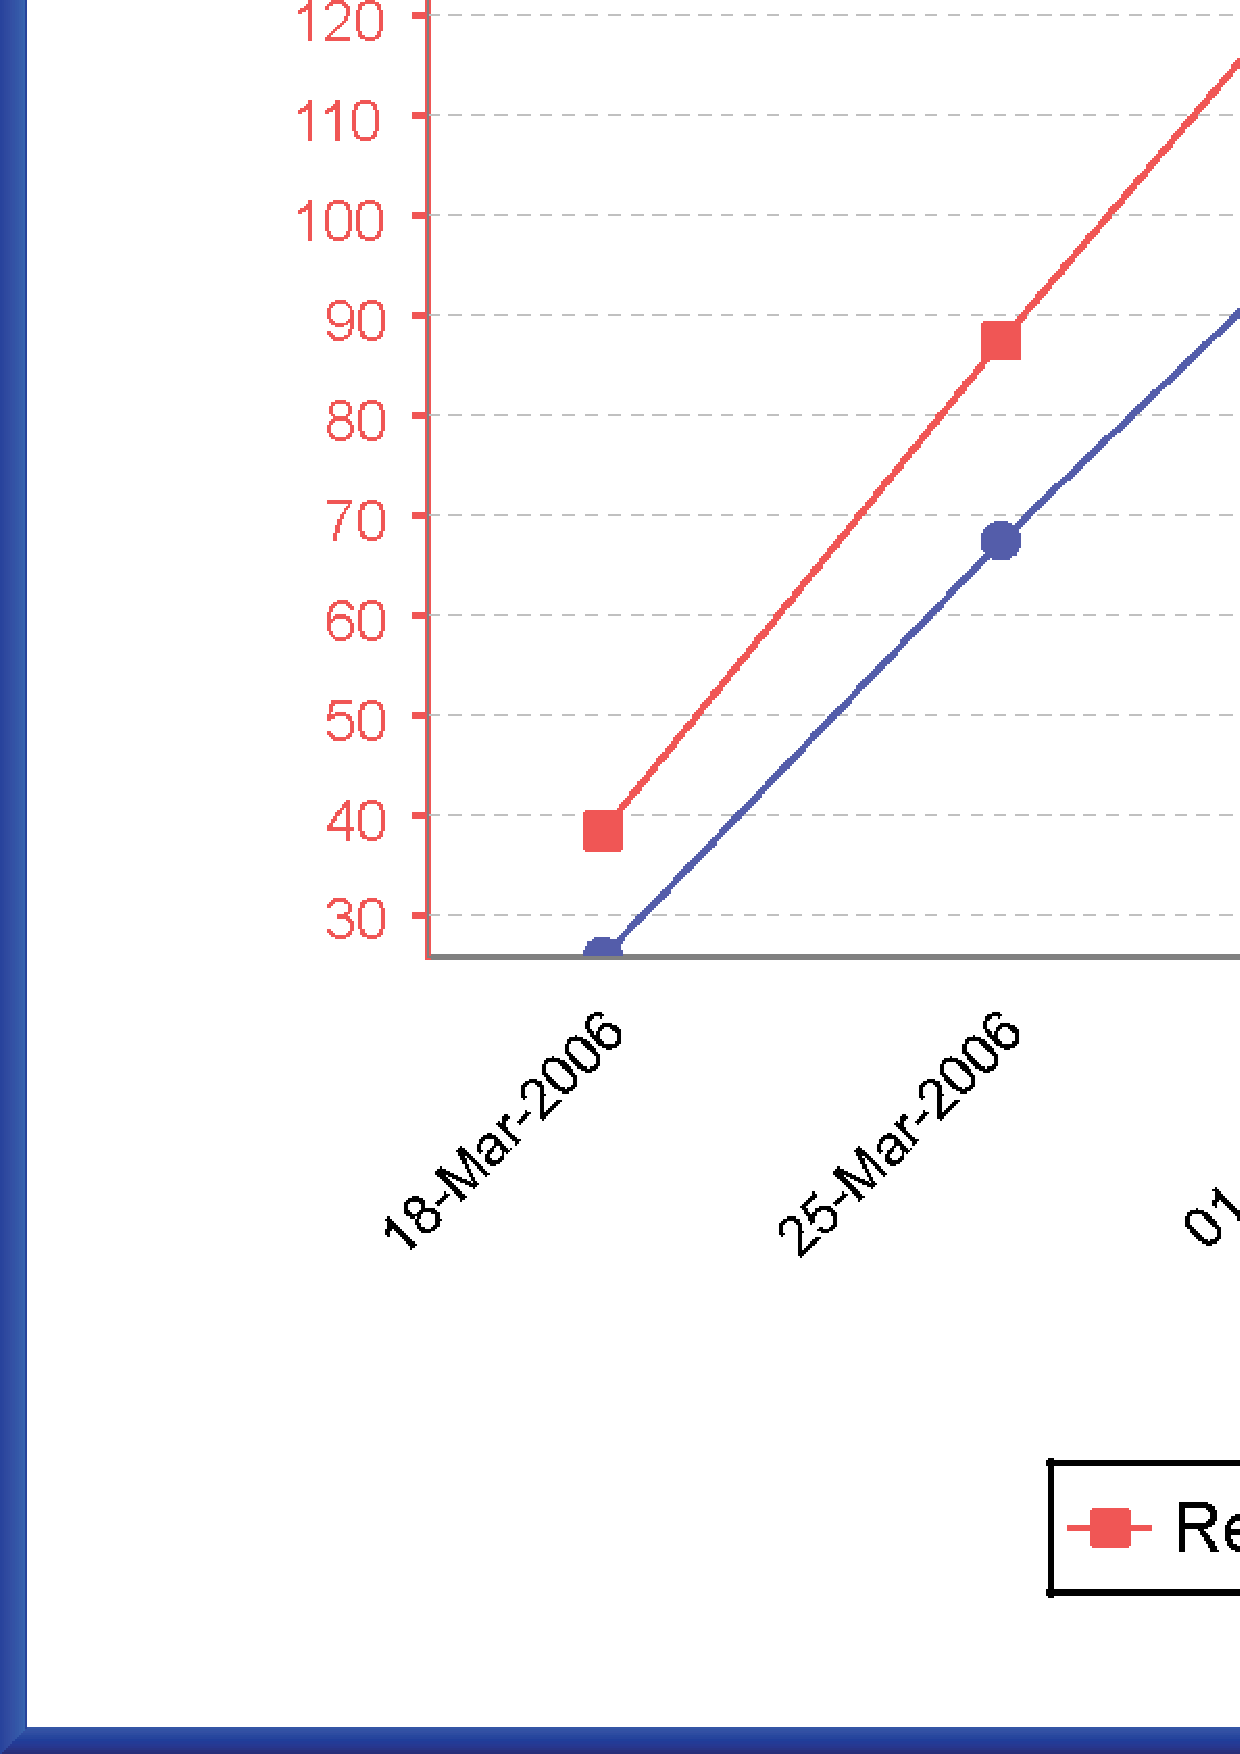
\includegraphics[width=0.70\textwidth]{figures/CSDL-IssueActiveTime740}
  \caption{Hackystat Release Cycle 7.4 --- Total Issues vs. Active Time} 
  \label{fig:CSDL-IssueActiveTime740}
\end{figure}

 









%%%%%%%%%%%%%%%
%  S T O R Y  %
%%%%%%%%%%%%%%%
\clearpage
%\subsection{Software project telemetry helped improve CSDL code quality.}
\subsection{Improvement on CSDL Code Quality}
\label{EvaluationInCSDL:EventsDescription:CodeIssue}

\subsubsection{Pre-hypothesis Data:}
\begin{itemize}
  \setlength{\itemsep}{0pt}
  \setlength{\parskip}{0pt}
  \item 2006-01-09-1: I asked a developer about his perception of the utility of the metrics currently collected in the lab during an interview. He told me that FindBugs reported too many problems, and that a lot of them were false-positive.
  \item 2006-01-11-1: I asked another developer about his perceptions about the utility of the metrics currently collected in the lab. He told me that metrics from FindBugs and PMD were not useful, but they could be made useful if the false-positive problem could be resolved. 
  \item 2006-01-16-1: In the weekly status meeting, the developers commented on the metrics from FindBugs and PMD. They all appeared to agree that there were too many false-positive warnings.
  \item 2006-02-09-2: CSDL deployed FindBugs and PMD sensors, even though the false-positive issue had not been addressed.
  \item 2006-03-23-1: I made the code issue density charts, which were computed from FindBugs and PMD metrics, available on the telemetry wall. I showed the charts to two of the developers. They told me that the charts failed to provide clue about Hackystat code quality, because they did not know the rules used by FindBugs and PMD to generate warnings. 
\end{itemize}

\subsubsection{Generated Hypothesis:}

The FindBugs and PMD warnings would be useful in improving Hackystat code quality, if the false-positive problem could be resolved. Since the development team in CSDL did not have enough resource to examine every single warning, the key to benefit from the tools was to prioritize the warnings they produced. Assuming different types of warnings had different probability of being false-positive, this probability could be used to determine the priority of the warnings.

\subsubsection{Intervention:}

I started with FindBug warnings and categorized them into three groups with different treatment options: \textit{fail}, \textit{monitor}, and \textit{ignore}.

\subsubsection{Post-hypothesis Data:}
\begin{itemize}
  \setlength{\itemsep}{0pt}
  \setlength{\parskip}{0pt}
%  \item 2006-04-17: I conducted a poll before the weekly status meeting. After 3 months FindBug and PMD were deployed, none of the developers had spent over one hour reading the FindBugs and PMD report, which the project manager had only spent 2-3 hours. The number suggested that their opinions were mostly preconceived.
  \item 2006-04-17-3: I discussed with the developers treatment options for each of the 17 types of FindBugs warnings found in hackyCore\_Kernel module in the weekly status meeting. The comments from the developers indicated that they had learned a lot by going over their own code that generated the warnings.
  \item 2006-04-24-1: I discussed with the developers treatment options for the remaining types of FindBugs warnings found in the Hackystat source in the weekly status meeting.
  \item 2006-04-25-1: I modified the code issue telemetry chart to track the number of warnings falling into ``fail'' and ``monitor'' categories.
  \item 2006-04-26-2: The project manager assigned tasks for the developers to get rid of the warnings that fell into the ``fail'' category.
  \item 2006-05-06-1: Telemetry analysis indicated that all the FindBugs warnings in the ``fail'' category had been eliminated, and the warnings in the ``monitor'' category had been reduced by more than a half.
\end{itemize}

\subsubsection{Conclusion:}

The additional data appears to confirm the hypothesis. The intervention was successful. Within two weeks, the developers had completely eliminated the FindBugs warnings in the \textit{``fail''} category, and drove down the FindBugs warnings in the \textit{``monitor''} category by more than a half.

\subsubsection{Elaboration:}

%This subsection reports on a successful experience of how I made \textit{``CodeIssue''} metrics useful as one of the code quality indicators, and helped the developers reduce a significant number of potential buggy code in the \textit{Hackystat} source. 

The \textit{``CodeIssue''} metric is a type of metric designed for representation of problems uncovered by static code analysis tools such as FindBugs\cite{Software:FindBugs} and PMD\cite{Software:PMD}. These tools perform static analysis either on Java source code or compiled byte code, and flag suspicious language constructs, which are potential software bugs. For example, a compiler won't complain if you try to dereference a null pointer, but when executing the code the most probable outcome is application crash.  

In February 2006, CSDL deployed both FindBugs and PMD to run on the Hackystat source. Unlike a compiler where the distinction between bug and non-bug is clear, these static code analyzers can only make probability statements about potential bugs. The general feeling among the developers was that there were too many warnings reported by the tools, and that most of them were false-positive. The telemetry chart in Figure \ref{fig:CSDL-FindBugs-PMD} indicated that in the nine weeks from Feb 25 to April 22, the number of warnings reported by FindBugs had increased from 507 to 518, while the number reported by PMD had increased from 6167 to 6702. The trends looked bad, but nobody was sure whether they constituted proof that the quality of the project had indeed gone down. One developer commented: \textit{``These numbers are potentially useful, but I don't think there are really useful at this time. There are so many false-positives.''} 

My hypothesis was that the warnings reported by FindBugs and PMD contained valuable information to improve Hackystat code quality. Since the development team in CSDL did not have enough resource to examine every single warning, the key to benefit from the tools was to prioritize the warnings they produced. Assuming different types of warnings had different probability of being false-positive, this probability could be used to determine the priority of the warnings.
Based on this hypothesis, I decided to put them into three categories with different treatment options: 

\begin{itemize}
	\item \textbf{Fail} ---- These were the types of warnings with high probability of being true. The existence of such warnings should fail CSDL nightly integration build, so that they could be eliminated immediately after they were detected.
	
	\item \textbf{Monitor} ---- These were the types of warnings with moderate probability of being true. They did not have to be dealt with immediately given the resource constraint faced by CSDL development team. However, the number of these types of warnings should be used as quality indicator and closely monitored for bad trend.

	\item \textbf{Ignore} ---- These were the types of warnings with low probability of being true. The development team should not waste any resource on them.
\end{itemize}

I started with FindBug warnings. For each type of warning, I picked one instance and discussed treatment options with the developers in CSDL weekly meetings. The discussion was overwhelmingly welcomed. The developers told me that they learned a lot about best coding practices to avoid common errors with the samples of warnings generated from their own code.
 
Figure \ref{fig:CSDL-FindBugs} is a telemetry chart showing the number of FindBugs warnings that fell into \textit{``fail''} and \textit{``monitor''} categories respectively. The chart indicated that within two weeks after the discussion, the developers had completely eliminated the warnings in the \textit{``fail''} category, and drove down the number of warnings in the \textit{``monitor''} category by more than a half. The project manager was so happy with the results, that he told me he would follow my approach to do the same thing with PMD warnings after the summer. 

\begin{figure}[p]
  \center
  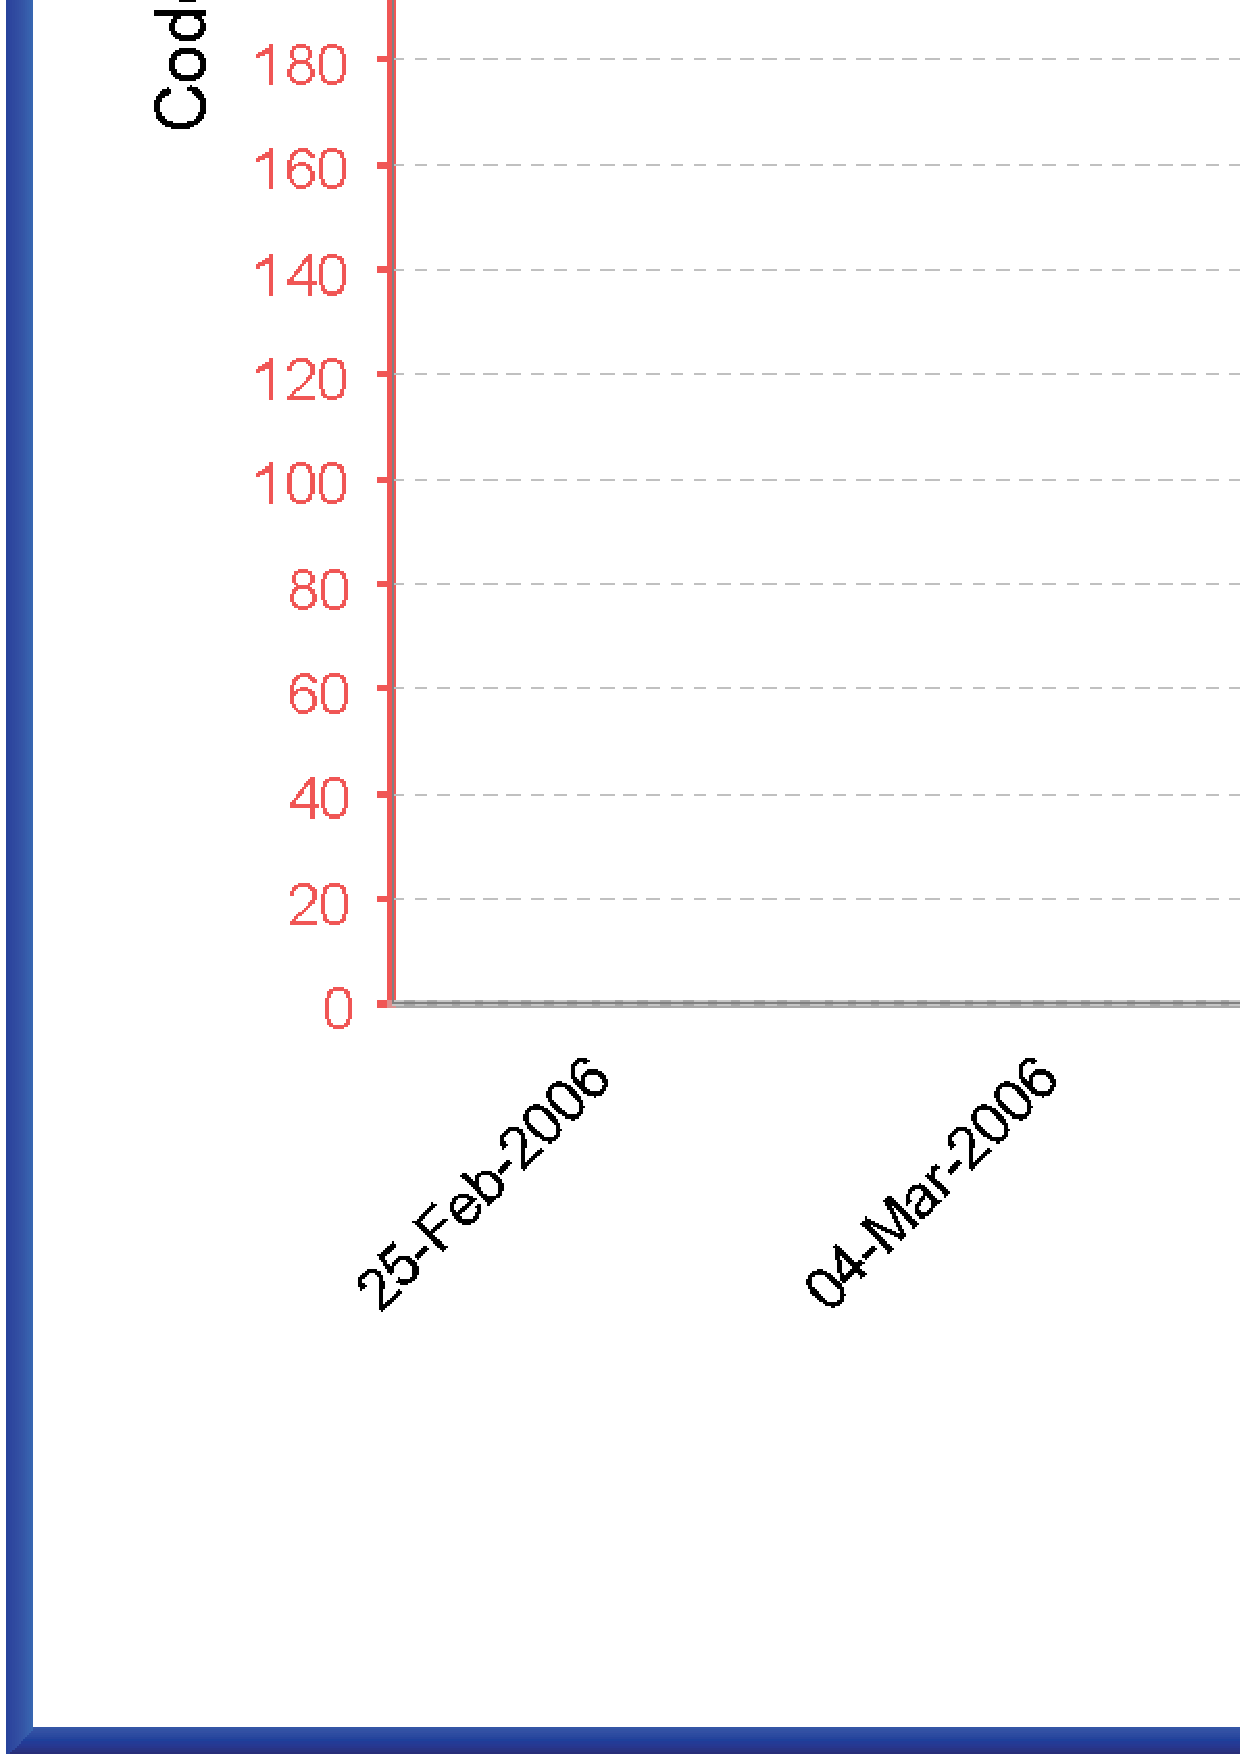
\includegraphics[width=0.70\textwidth]{figures/CSDL-FindBugs-PMD}
  \caption{FindBugs and PMD Warnings from the Hackystat Source} 
  \label{fig:CSDL-FindBugs-PMD}
\end{figure}

\begin{figure}[p]
  \center
  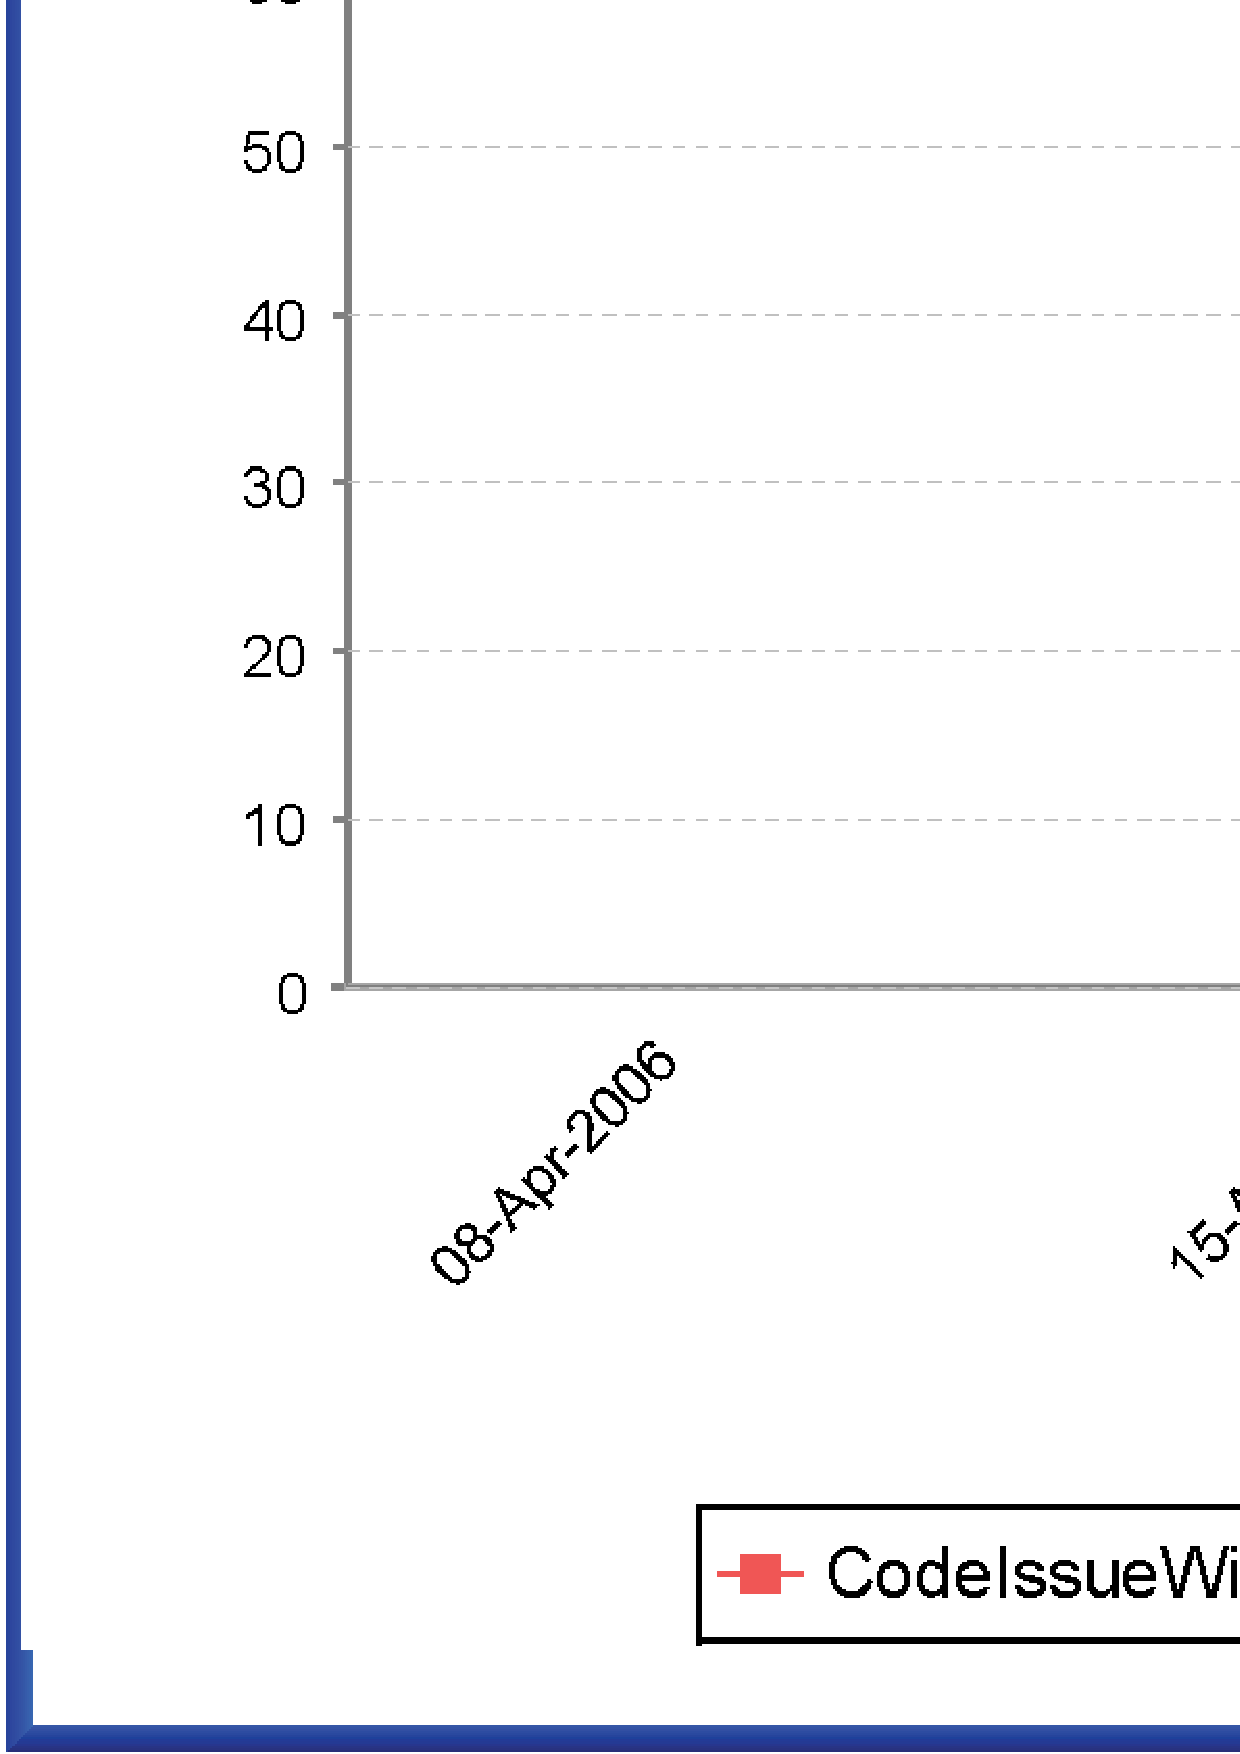
\includegraphics[width=0.70\textwidth]{figures/CSDL-FindBugs}
  \caption{FindBugs Warnings in ``Fail'' and ``Monitor'' Categories} 
  \label{fig:CSDL-FindBugs}
\end{figure}










%%%%%%%%%%%%%%%
%  S T O R Y  %
%%%%%%%%%%%%%%%
\clearpage
%\subsection{Software project telemetry provided the developers with insights into their processes.}
\subsection{Improvement on Developers' Insights into their Software Development Process}
\label{EvaluationInCSDL:EventsDescription:BuildAnalysis}

\subsubsection{Pre-hypothesis Data:}

The pre-hypothesis data came from a previous study in which I analyzed 2004 CSDL integration build failure data. The study found that the build failure rate was significant. The loss of productivity due to the integration build failures was substantial, since each build failure generally required one or more developers to stop concurrent development, diagnose the problem, and determine who was responsible for fixing the error. Often times, other developers had to wait until the corrections were made before they could check out or commit additional code. The study suggested that the causes of the integration build failures were quite complex. They involved at least the following: developer's familiarity with the system, the actual changes made to the code, the dependency relationships among the modules. Since there was no statistical correlation between integration build failures and the number of lines of code committed or the amount of active time spent before the commit, it would be difficult to adopt the traditional approach of building an analytical model to predict the probability of integration build failure in order to forewarn the developers. At the same time, the study also suggested that 74\% -- 82\% of the intergration build failures were preventable if the developers could build and test the system on their workstations before committing the changes to the repository. However, there is a dilemma. On the one hand,  the developers often do not test their changes against the entire code base before committing them, because a full build and test could take over 15-20 minutes, which would be quite time-consuming given that the developers often commit more than once a day. On the other hand, the cost of a broken build is quite time-consuming too, since it could prevent other developers from working when the code repository is in an inconsistent state.

\subsubsection{Generated Hypothesis:}

Software project telemetry could be used to provide feedback to the developers to help them gain insights into their software development processes and the cost associated with integration build failures, so that they could learn from their past experiences to test ``just the right amount'' of the system before committing their changes, where ``just the right amount'' involves a trade-off between local quality assurance effort and increased risk of an integration build failure.
%through making trade-off decisions between reducing local quality assurance effort and reducing integration build failure cost. 

\subsubsection{Intervention:}

Software project telemetry was used to provide process feedback to the developers. To draw their attention, I implemented an email alert that automatically identified the plausible developer responsible for the build failure whenever possible.

\subsubsection{Post-hypothesis Data:}
\begin{itemize}
  \setlength{\itemsep}{0pt}
  \setlength{\parskip}{0pt}
  %\item 2006-01-06: During an interview with a developer, he told me that he did not care about the details of integration build failures unless it was caused by him.
  %\item 2006-01-06: During an interview with another developer, he told me that he did not care about the details of integration build failures unless it was caused by him. 
  %\item A developer break the build, was identified correctly, but blamed others.
  
  \item 2006-01-19-2: I interviewed a developer (developer 1) who was identified as responsible for a recent integration build failure. I asked him how it might impact his local quality assurance practice. He told me that it was \textit{``very effective''} in making him think more about the integration build result when committing changes.%P
  
  \item 2006-01-31-2: I interviewed a developer (developer 2) on the impact of the integration build failure alert mechanism. He commented that it made him \textit{``a little bit more cautious''} when committing changes. %He commented: ``it changed my process a little bit.'' %M
  
  \item 2006-01-31-3: I interviewed developer 1 on the impact of the integration build failure email alert mechanism. He commented: \textit{``you might be identified as a culprit, (which) tends to make you try a little harder to think about when you actually do the thing (i.e., committing changes).''} %P
  
  \item 2006-02-02-3: I interviewed a developer (developer 3) on the impact of the integration build failure alert mechanism. He told me that his behavior was changed significantly from \textit{``I just build the module to see if it works''} to \textit{``I build the entire system and test every time before commit.''} %A
  
  \item 2006-02-02-4: I interviewed a developer (developer 4) on the impact of the integration build failure alert mechanism. He told me that it had not changed his behavior because he was always careful about local quality assurance. %J
  
  \item 2006-03-08-1: I interviewed a developer (developer 5) on the impact of the integration build failure alert mechanism. He told me that he had spent more time on local quality assurance than before. There was overhead, but it was acceptable since it would be much more troublesome to have integration build failures. %H
  
  \item 2006-03-08-2: I interviewed developer 4. He controlled the local quality assurance overhead by reducing the number of commits. %J
  
  \item 2006-03-14-2: I interviewed developer 2. He commented that the overhead on local quality assurance was acceptable give the consequence of integration build failures. He controlled the overhead by reducing the number of commits. %M
  
  %\item 2006-03-22: I provide the project manage a table list all past build failures and asked him to determine which ones are acceptable and which are not. It seemed his criteria also involves trade-off.
  
  \item 2006-03-23-1: I discussed the telemetry charts on integration build failures and various software development process metrics with two of the developers. They confirmed that integration build failure was a complex phenomenon, and that it would be very hard, if not impossible, to predict the probability from the process metrics. 
  
\end{itemize}

\subsubsection{Conclusion:}

The post-hypothesis data appears to confirm the hypothesis. By providing process feedback to the developers, software project telemetry seemed to make them more aware of the cost associated with integration build failures and thus more careful when committing their changes.
Analysis of the developer's process metrics and integration build failure trends (Figure \ref{fig:CSDL-CorrelationAnalysis}) seemed to confirm that they were learning from their past experiences and getting \textit{``smarter''} about their local quality assurance practices.

\subsubsection{Elaboration:}

The Hackystat project is so large that the developers usually work on a subset of the modules relevant to their assignments. An automated integration build tool is used in CSDL to build and test the entire code to make sure that the developers' modifications do not break the system. The process is illustrated in Figure \ref{fig:BuildProcess} and discussed in Section \ref{EvaluationInCSDL:Setting}. 
In early 2005, I conducted a study on CSDL integration build failures using 2004 data. The study suggested that the causes of the integration build failures were quite complex, which involved many factors, such as developer's familiarity with the system, the actual changes made to the code, the dependency relationships among the modules, etc. As a result, I was unable find statistical correlation that could be used describe the causal relationship between software development practices and integration build failures in CSDL.
However, the study did suggest there was a trade-off between developers' local quality assurance effort and integration build failures. Testing the changes against the entire code base before committing them could reduce the integration build failure rate significantly, but it was quite time-consuming. On the other hand, a failed integration build would often waste other developer's time because the code in the repository was in a unsafe state.

My hypothesis in this study was that the phenomena of software development practices and integration build failures are so complex that it would be futile to build a predictive model to describe the causal relationship between them. Instead, software project telemetry could be used to provide feedback to the developers to help them gain insights into their software development processes and the cost associated with integration build failures, so that they could learn from their past experiences to test ``just the right amount'' of the system before committing their changes, where ``just the right amount'' involves a trade-off between local quality assurance effort and increased risk of an integration build failure. In order to draw their attention to telemetry analysis results, I implemented an email alert that automatically identified the plausible developer responsible for the build failure whenever possible.

The data in this study indicated that the result was positive. The responses from the developers (see post-hypothesis data) seemed to suggest that software project telemetry made them more aware of the cost associated with integration build failures. As a result, they seemed to be more careful about committing their changes, and more effort was spent on local quality assurance.

The phenomena resembled the typical textbook case of game theory in Economics. Consider a hypothetical game Adam and Bob are playing, in which each player has two choices: choice 1 and 2. The payoff matrix is listed in Table \ref{table:NashEquilibrium}. Now consider what would happen if Adam and Bob cannot communicate with each other. If Adam's choice is 1, then Bob's best response is 2 because he can get \$110 by choosing 2 instead of \$100 by choosing 1. On the other hand, if Adam's choice is 2, then Bob's best response is still 2 because he can get \$10 by choosing 2 instead of \$0 by choosing 1. In other words, Bob's best response is always 2 regardless of Adam's choice. If you apply the same logic to Adam, then you would find that Adam's best response is always 2 regardless of Bob's choice. Therefore, both Adam and Bob would end up with \$10 when they cannot communicate with each other, and thus cannot reach a mutually beneficial deal.\footnote{This is what is called Nash equilibrium in Economics. A much more complex version of it is often used to model market outcome in a duopoly competition.} Both players act rationally trying to maximize his own benefit. However, obviously, rational decisions are not always optimal, because if Adam and Bob could reach a binding agreement, then both of them would end up much better off by getting \$100 each. 

\begin{table}[tbp]
	\centering
		\caption{Nash Equilibrium in a Non-Cooperative Game}
		\begin{tabular}{|p{0.20\textwidth}|p{0.20\textwidth}|p{0.18\textwidth}|} 
			\hline
			{} & \textbf{Bob Choosing 1} & \textbf{Bob Choosing 2} \\
			\hline
			\textbf{Adam Choosing 1} & -- Adam gets \$100; -- Bob gets \$100. & -- Adam gets \$0 ; -- Bob gets \$110. 
			\\
			\hline
			\textbf{Adam Choosing 2} & -- Adam gets \$110; -- Bob gets \$0. & -- Adam gets \$10; -- Bob gets \$10. 
			\\
			\hline
		\end{tabular}
	\label{table:NashEquilibrium}
\end{table}

Put it in the context of CSDL, I can hypothesize that the developers were always making rational decisions to reduce their software development effort. Before the introduction of software project telemetry, they were less aware of the productivity loss of the integration build failures incurred by other developers, and their decisions were more or less focused on minimizing local quality assurance effort. As a result, they ended up in the low payoff position. On the other hand, the process feedback mechanism I introduced with software project telemetry made them more aware of the cost associated with the integration build failures, and they began to make trade-off decisions to minimize the total combined cost instead of only local quality assurance cost. As a result, though the local quality assurance effort as experienced by individual developers had increased, the entire team were actually moving toward the high payoff position. 

Figure \ref{fig:CSDL-CorrelationAnalysis} provides evidence that the developers were learning to make trade-off decisions between reducing local quality assurance cost and reducing integration build failure cost in order to minimize the total cost.
The first chart shows the number of integration build failures in each month from January to April 2006. 
The second chart shows the number of times that the build script was invoked by the developers on their workstations. A typical purpose was to test the modifications locally before committing them to the repository.
The last chart showed three telemetry streams on \textit{FileCommit}, \textit{CodeChurn}, and \textit{ActiveTime}. \textit{FileCommit} measures the total number of files in all commits from all developers. \textit{CodeChurn} is related to file commit. It computes the total number of lines added and deleted in each revision. \textit{ActiveTime} computes the amount of time a developer spent actively editing code inside an IDE. They all measure software development effort except from different angles.

It seemed that the developers were learning from their past experiences and getting \textit{``smarter''} about their processes. January was the month with low development effort, large amount of local testing, and low integration build failures. It seemed to suggest that low integration build failure was achieved at the cost of lots of local tests. In February, development effort went up with no significant change in local testing pattern, resulting in higher number of integration build failures. March was the month with high development effort, moderate integration build failure rate, and very low local testing effort. This seemed to support the hypothesis that the developers had learned from their past experiences to test ``just the right amount'' of the system before committing their changes.

On a cursory look, the April data seemed contradictory to that hypothesis, with extremely high rate of integration build failure. But further investigation indicated that the April data were not directly comparable. April was the time that CSDL embarked on a completely different type of software development task: the team were busy with updating the Hackystat infrastructure code to support sensor data type evolution. The integration build failures concentrated on several non-actively-maintained leaf modules that were not in the developers' working set. They were exactly the type of build failures the integration build system was designed to detect. My CSDL study ended in early May, but I can conjecture that with continued metrics collection, I would find evidence that the developers are beginning to learn to deal with the new situation and bringing integration build failure back under control. 

\begin{figure}[p]
  \center
  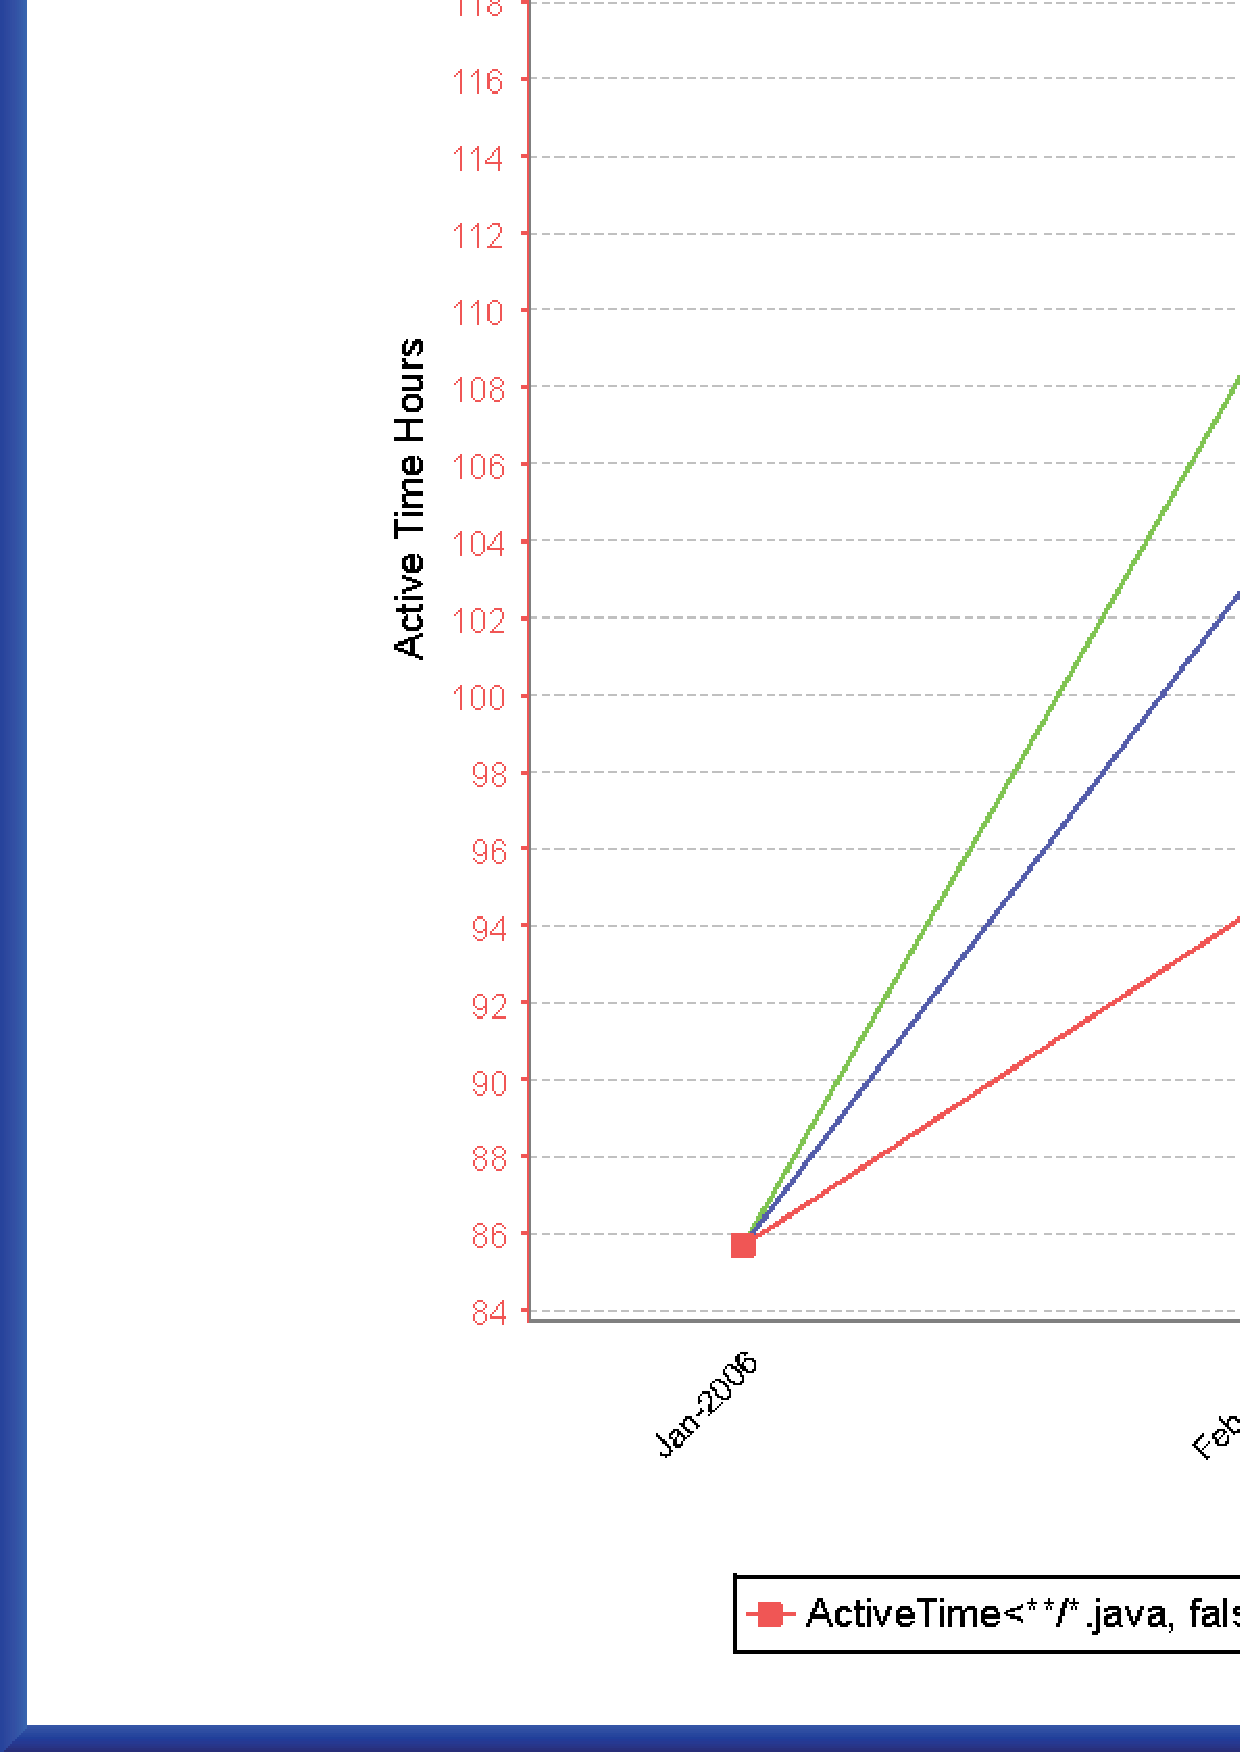
\includegraphics[width=0.67\textwidth]{figures/CSDL-CorrelationAnalysis}
  \caption{Integration Build Failures and Process Metrics} 
  \label{fig:CSDL-CorrelationAnalysis}
\end{figure}












%%%%%%%%%%%%%%%
%  S T O R Y  %
%%%%%%%%%%%%%%%
\clearpage
%\subsection{Top-down telemetry design is a best practice.}
\subsection{Top-down Telemetry Design}
\label{EvaluationInCSDL:EventsDescription:TopDownDesign}

\subsubsection{Pre-hypothesis Data:}
\begin{itemize}
  \setlength{\itemsep}{0pt}
  \setlength{\parskip}{0pt}
  \item 2006-01-16-1: In a weekly status meeting, the developers noted that one could generate a lot of telemetry charts using the telemetry language. But they also asked: \textit{``do we really care about all those charts?''}
  %\item 2006-02-01: \textcolor{red}{The project manager sent me an email regarding what he wishes to see on the telemetry wall.}
	\item 2006-02-05-1: I gathered a list of the types of metrics collected in CSDL, and generated telemetry charts to show how these metrics changed over time in different grain size. The telemetry wall was up.
	\item 2006-02-06-1: I introduced the telemetry wall in the weekly status meeting, but the project manager and the developers found that most of the charts were not useful, except the release cycle issue tracking charts. They gave me a list of questions that they wished telemetry charts could help shed light on, such as some notion of quality indicators for each module in the project.
\end{itemize}

\subsubsection{Generated Hypothesis:}
The telemetry charts generated in a bottom-up fashion (i.e., organized by the types of metrics) were generally not useful, because they were not designed with any purpose in mind. You cannot expect the project manager or the developers to fish around hundreds of charts to find the ones that are useful to them. The reason that the issue tracking charts were found useful was because they happened to have a purpose: allowing the manager to track progress in a release cycle. Therefore, useful telemetry charts are those that are designed with a specific top-level goal in mind.

\subsubsection{Intervention:}
I redesigned the telemetry charts for the telemetry wall, organizing them by their intended use (i.e., top-down design). For example, there was a scene (a set of related charts displayed together on the telemetry wall) for release cycle issue tracking, and there was another scene for module level quality indication.

\subsubsection{Post-hypothesis Data:}
\begin{itemize}
  \setlength{\itemsep}{0pt}
  \setlength{\parskip}{0pt}
  \item 2006-02-21-2: I discussed the top-down designed charts with three of the developers, and they thought the charts displayed useful information.
	\item 2006-02-22-1: I showed the charts to the project manager, and he liked them.
	\item 2006-03-07-1: After receiving complaints about missing coverage data, the project manager sent me an email asking whether it would be possible to design charts to help detect sensor malfunction.	
	\item 2006-03-09-1: A set of charts specifically designed for the purpose of verifying developer-side process metrics were deployed on the telemetry wall. Immediately, I noticed that one of the developers had missing data. It turned out that the developer reinstalled the IDE but forgot to reattach the sensor.
	\item 2006-03-17-1: The project manager was so impressed with the utility of those top-down designed telemetry charts on the telemetry wall, that he decided to devote an entire page on the Hackystat website to publish the results.
\end{itemize}

\subsubsection{Conclusion:}
The additional data appears to confirm the hypothesis. Though \textit{``bottom-up telemetry design''} based on the types of metrics can generate hundreds of charts without significant effort, the charts lack clear purposes and are generally of little value to users. \textit{``Top-down telemetry design''} based on user goals, which is similar to the idea in the Goal-Question-Metric paradigm, yields useful telemetry charts.

\subsubsection{Elaboration:}

At the beginning of this study, I used bottom-up approach to generate telemetry charts to be displayed on the telemetry wall. I gathered a list of the types of metrics collected in CSDL, and then generated charts to show how these metrics change over time in different grain sizes with possible breakdown to individual developer or individual source code module. The charts were organized by the types of metrics. For example, a scene on the telemetry wall might be displaying charts all related to \textit{active time}, and another scene might be displaying charts all related to \textit{code issue} density.

With the bottom-up approach, hundreds of charts could be easily generated. I introduced them in a weekly status meeting. However, I found that most of them were not useful. 
A frequent question the project manager and the developers asked during my presentation was: \textit{``Why would that be of use to me?''} The only exception was the charts related to release cycle issue tracking, which the project manager found \textit{``highly useful.''}
Further discussion revealed that the project manager and the developers had a number of questions they wished software project telemetry could shed light on, such as:
\begin{itemize}
	\item \textit{``Could telemetry help me identify the situation where the sensors are likely not being installed?''}
	\item \textit{``Could telemetry offer some notion of quality so that it helps me locate the modules with low quality, or the modules that are changing with respect to quality?''}
	\item \textit{``Could telemetry give me a sense of how we are making progress toward the stable release?''}
\end{itemize}

My hypothesis was that bottom-up telemetry design was unsuccessful because it generated hundreds of charts organized by metrics types. You just cannot expect users to go over all those charts to find the ones that are useful to them. The issue tracking charts were useful because they happened to serve a purpose: they enabled the project manager to track progress in a release cycle. In order for other charts to be useful, they have to be re-organized in a top-down fashion by the questions they intended to answer. 
%\textcolor{red}{In fact, the project manager already state what he wished to see. 2006-02-01. I did not pick up the hint, and continued to use bottom-up approach.}
Based on this hypothesis, I redesigned the telemetry charts following top-down approach, which resulted in a number of successful telemetry scenes being displayed on the telemetry wall:

\begin{itemize}
  \setlength{\itemsep}{0pt}
  \setlength{\parskip}{0pt}
	\item A telemetry scene for release cycle issue tracking.
  \item A telemetry scene for product metrics at project level for quality indication.
  \item A set of telemetry scenes for product metrics at module level for quality indication. One scene per module.
  \item A telemetry scene for module filtering to discover interesting information in a large project like \textit{Hackystat}.
  \item A telemetry scene for software development process metrics and correlation analysis.
  \item A telemetry scene for sensor data verification.
\end{itemize}

The top-down designed telemetry charts were so successful that the project manager decided to devoted an entire page on Hackystat website to publish the results. A snapshot is captured in Figure \ref{figures/TelemetryReport-Page1} and \ref{figures/TelemetryReport-Page2}. The URL of the web page is:
\begin{quotation}
	\textit{http://www.hackystat.org/hackyDevSite/telemetryReport.do}
\end{quotation}

The web page contains a collection of both \textit{historical} and \textit{real-time} charts, which serves two purposes: 
(1) enabling the entire Hackystat developer community, especially those off-site developers, to monitor the project development status, and (2) demonstrating the power of the Hackystat framework by showing the achievement of one of its extensions.

\begin{figure}[p]
  \center
  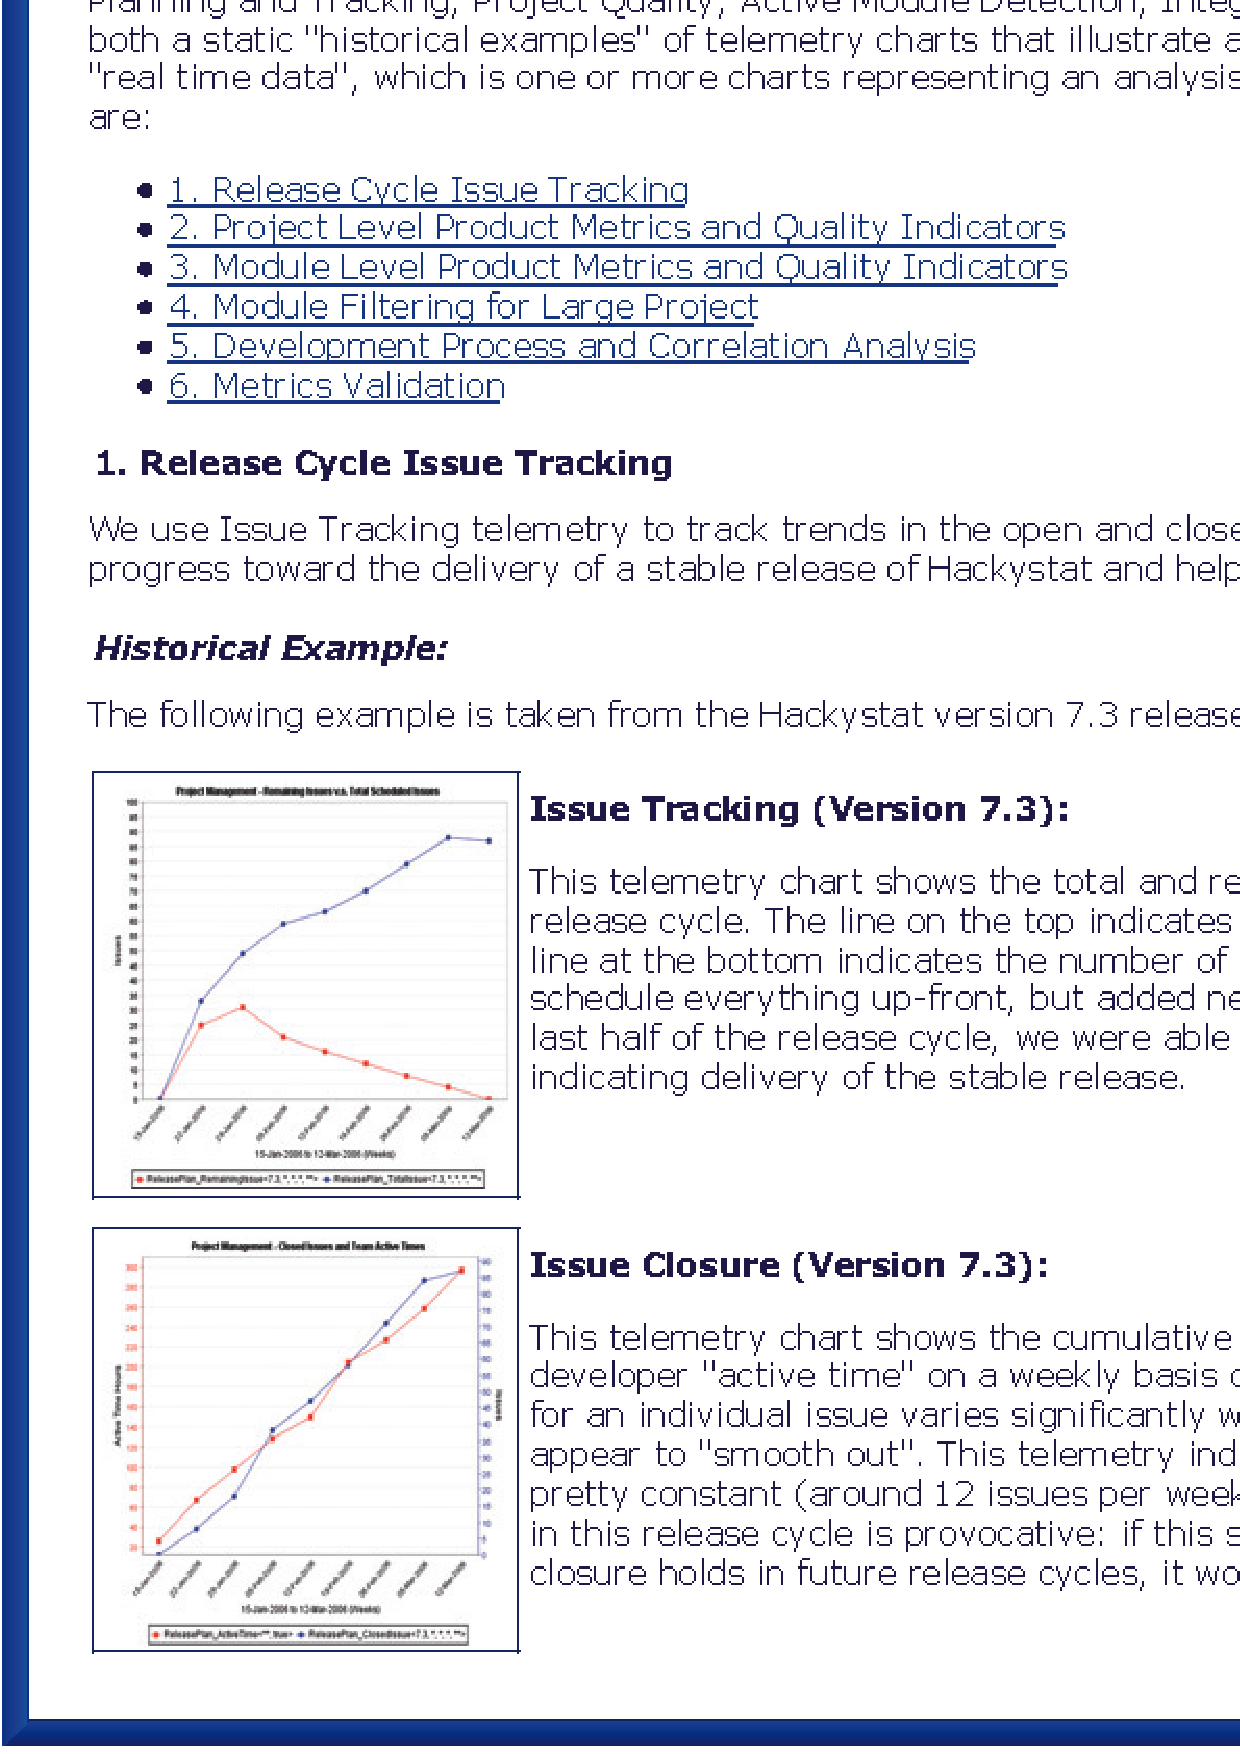
\includegraphics[height=0.93\textheight]{figures/TelemetryReport-Page1}
  \caption{Telemetry Report: Page 1} 
  \label{figures/TelemetryReport-Page1}
\end{figure}

\begin{figure}[p]
  \center
  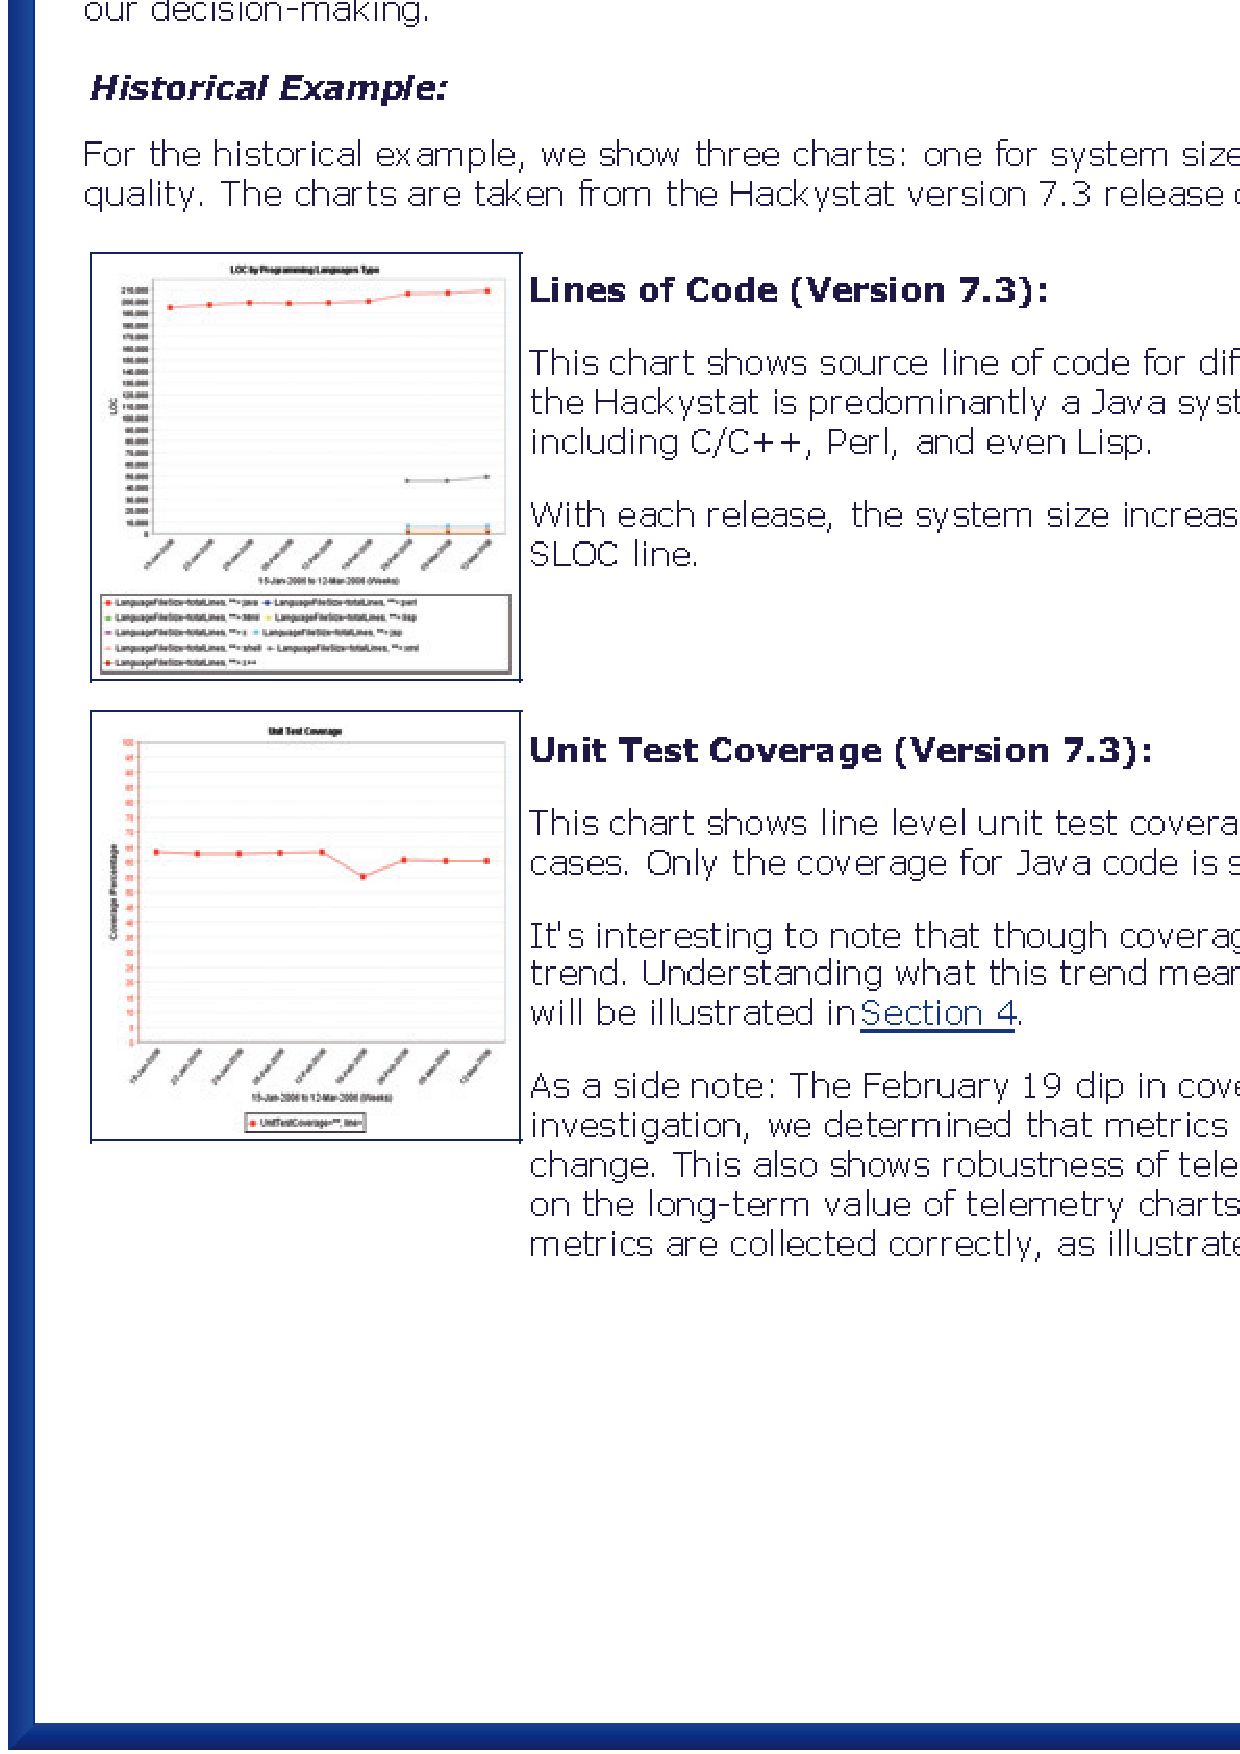
\includegraphics[height=0.93\textheight]{figures/TelemetryReport-Page2}
  \caption{Telemetry Report: Page 2} 
  \label{figures/TelemetryReport-Page2}
\end{figure}








%%%%%%%%%%%%%%%
%  S T O R Y  %
%%%%%%%%%%%%%%%
\clearpage
%\subsection{Using software project telemetry for sensor data self-verification is a best practice.}
\subsection{Sensor Verification}
\label{EvaluationInCSDL:EventsDescription:DataVerification}

\subsubsection{Pre-hypothesis Data:}
\begin{itemize}
  \setlength{\itemsep}{0pt}
  \setlength{\parskip}{0pt}
  \item 2006-01-31-4: I noticed an inconsistency in telemetry charts: there was no data from one of the developers. It turned out it was caused by a bad server-side project configuration.
  \item 2006-02-01-1: The same developer told me he had fixed the problem, but the inconsistency still existed in telemetry charts. The project was still mis-configured despite the developer's effort to fix it.
  \item 2006-02-06-1: During my presentation of telemetry charts in the weekly status meeting, I noticed that the developers were using some of the charts to assess whether the underlying sensors data seemed correct or not. Further discussion identified two common causes for incorrect sensor data: (1) sensor not working correctly, and (2) bad server-side project configuration.
\end{itemize}

\subsubsection{Generated Hypothesis:}

There is always possibility for incorrect sensor data. Ensuring sensor data correctness is a tedious and time-consuming process, because a developer has to log onto the server to compare raw sensor data entries with his expectations. Specially designed telemetry charts could save much of the effort by allowing a developer to make quick assessment of the likelihood of occurrence of sensor data problem.

\subsubsection{Intervention:}

I designed a set of sensor data verification charts, and made them available both on the telemetry wall and on the public Hackystat website.

\subsubsection{Post-hypothesis Data:}
\begin{itemize}
  \setlength{\itemsep}{0pt}
  \setlength{\parskip}{0pt}
  \item 2006-02-26-1: Telemetry charts showed missing coverage data. It turned out that the sensor configuration file was not updated when a developer added a new module.
  \item 2006-03-05-1: Telemetry charts showed missing issue metrics. It turned out that a developer forgot to update the project configuration when adding a new module.
  \item 2006-03-09-1: I added additional telemetry charts on the telemetry wall, designed to verify developer-side process metrics. Immediately, I detected that one developer has missing active time data. It turned out that the developer reinstalled the IDE but forgot to reattach the sensor.
  \item 2006-04-20-1: A developer modified Jira sensor code. Telemetry charts showed missing issue metrics. It turned out it was caused by a bug in the code.
  \item 2006-04-22-2: An email from the project manager indicated he detected the same Jira sensor problem using the real-time sensor verification charts on the public Hackystat website.    
\end{itemize}

\subsubsection{Conclusion:}

The data appears to suggest that it would be hard to avoid sensor data problem. The problem was most severe when a project's scope was changed, such as adding a new module. Nevertheless, specially designed telemetry charts are efficient at detecting the problem. It seems that the best practice would be to designate a person to spend one or two minutes each day to examine the charts for early detection of sensor data problem. 


\subsubsection{Elaboration:}

The central idea of sensor-based metrics collection is that sensors are designed to collect metrics automatically and unobtrusively. Once they are installed, they work silently in the background. It is very easy for a developer to forget about the existence of the sensors. At the same time, it also means that sensor data problem can go unnoticed for a long time. Bad sensor data are caused by many reasons, such as software bug, inappropriate sensor configuration, and server-side project configuration. Though telemetry analysis has greater tolerance for incorrect metrics compared to traditional model-based metrics approaches, complete and correct data still provide the best decision-making value. However, ensuring sensor data correctness is a tedious task. A developer has to log onto the server where raw sensor data are stored and compare the entries with his expectations. It typically involves thousands of sensor data entries on a project of the size like Hackystat.

A serendipitous discovery in this study was that there were several instances that inconsistencies in telemetry charts helped detect the underlying sensor data problem. 
My hypothesis was that these were not isolated events and that it was possible design telemetry charts to allow the developers to make quick assessment of the likelihood of the occurrence of sensor data problem. These charts could be used in a number of different ways:

\begin{itemize}
	\item \textbf{Detecting dropout of data points in telemetry streams:}

A dropout usually indicates that the sensor did not send the data. For some types of metrics, it is completely normal. For example, \textit{ActiveTime} is only generated when a developer is actively editing code inside an IDE. It is normal for it drop out for a few days because the developer might be taking a break. But a dropout of \textit{ActiveTime} for a prolonged period of time might be indicative of problem. For other types of metrics, any dropout signifies an error condition. For example, CSDL uses an integration build system to run unit tests and collect coverage metrics every night automatically. There should be no missing data point in coverage data stream if everything is working as expected.

	\item \textbf{Detecting outliers or sudden value changes in telemetry streams:}
	
An outlier or sudden value change is normal if it is caused by drastic change in software development process or software product. But, often times, it is an indication of sensor breakdown: sending incomplete or incorrect data to the server.

	\item \textbf{Detecting whether related metrics were changing together or not:}

Some related metrics should change together with each other. For example, in Figure	\ref{fig:CSDL-DeveloperSensorVerification}, active \textit{time}, \textit{build}, \textit{unit test}, and \textit{commit} are related because they all serve as proxy for software development effort. If one of them does not co-vary with the rest, it usually indicates that the sensor is not working correctly.
	
\end{itemize}

After I made the sensor data verification telemetry charts available, they supported early detection of several instances of sensor data problems. 
One instance involved Figure \ref{fig:CSDL-CoverageSensorVerification}, which showed a chart tracking unit test coverage. The chart was generated for the period from Feb 14 to Feb 26 on a daily interval. There was no unit test data after Feb 20. The sudden drop of coverage from 64\% to 55\% made it even more suspicious that something significant had occurred to the project around that day which broke the \textit{Emma} sensor.\footnote{\textit{``Emma''} sensor was the sensor CSDL used to collect unit test coverage information.} Further investigation revealed that one of the developers had created a new module, but forgot to update the configuration file to include that  module.

Another instance involved Figure \ref{fig:CSDL-DeveloperSensorVerification}, which showed a chart representing four types of metrics related to software development effort: the number of active time hours, the number of local builds, the number of unit test invocations, and the number of commits. The four types of metrics should all co-vary with each other, because they all represent software development effort albeit from different perspectives. For example, from Feb 16 to Mar 6, everything was normal. When active time was high, the other three types of metrics were high. When active time was low, the other three types of metrics were low. When active time was zero, the other three types of metrics were zero too. However, for the four days from Mar 7 to Mar 10, the metrics values were abnormal. The developer had build, unit test, and commit activities, but there was no active time. Further investigation revealed that the developer had reinstalled Eclipse IDE, but forgot to reattach the sensor.

The CSDL experience appears to suggest that it is almost impossible to avoid sensor data problem altogether, the best practice would be to designate a person to spend one or two minutes each day to examine the charts for early detection of sensor data problem. 

\begin{figure}[p]
  \center
  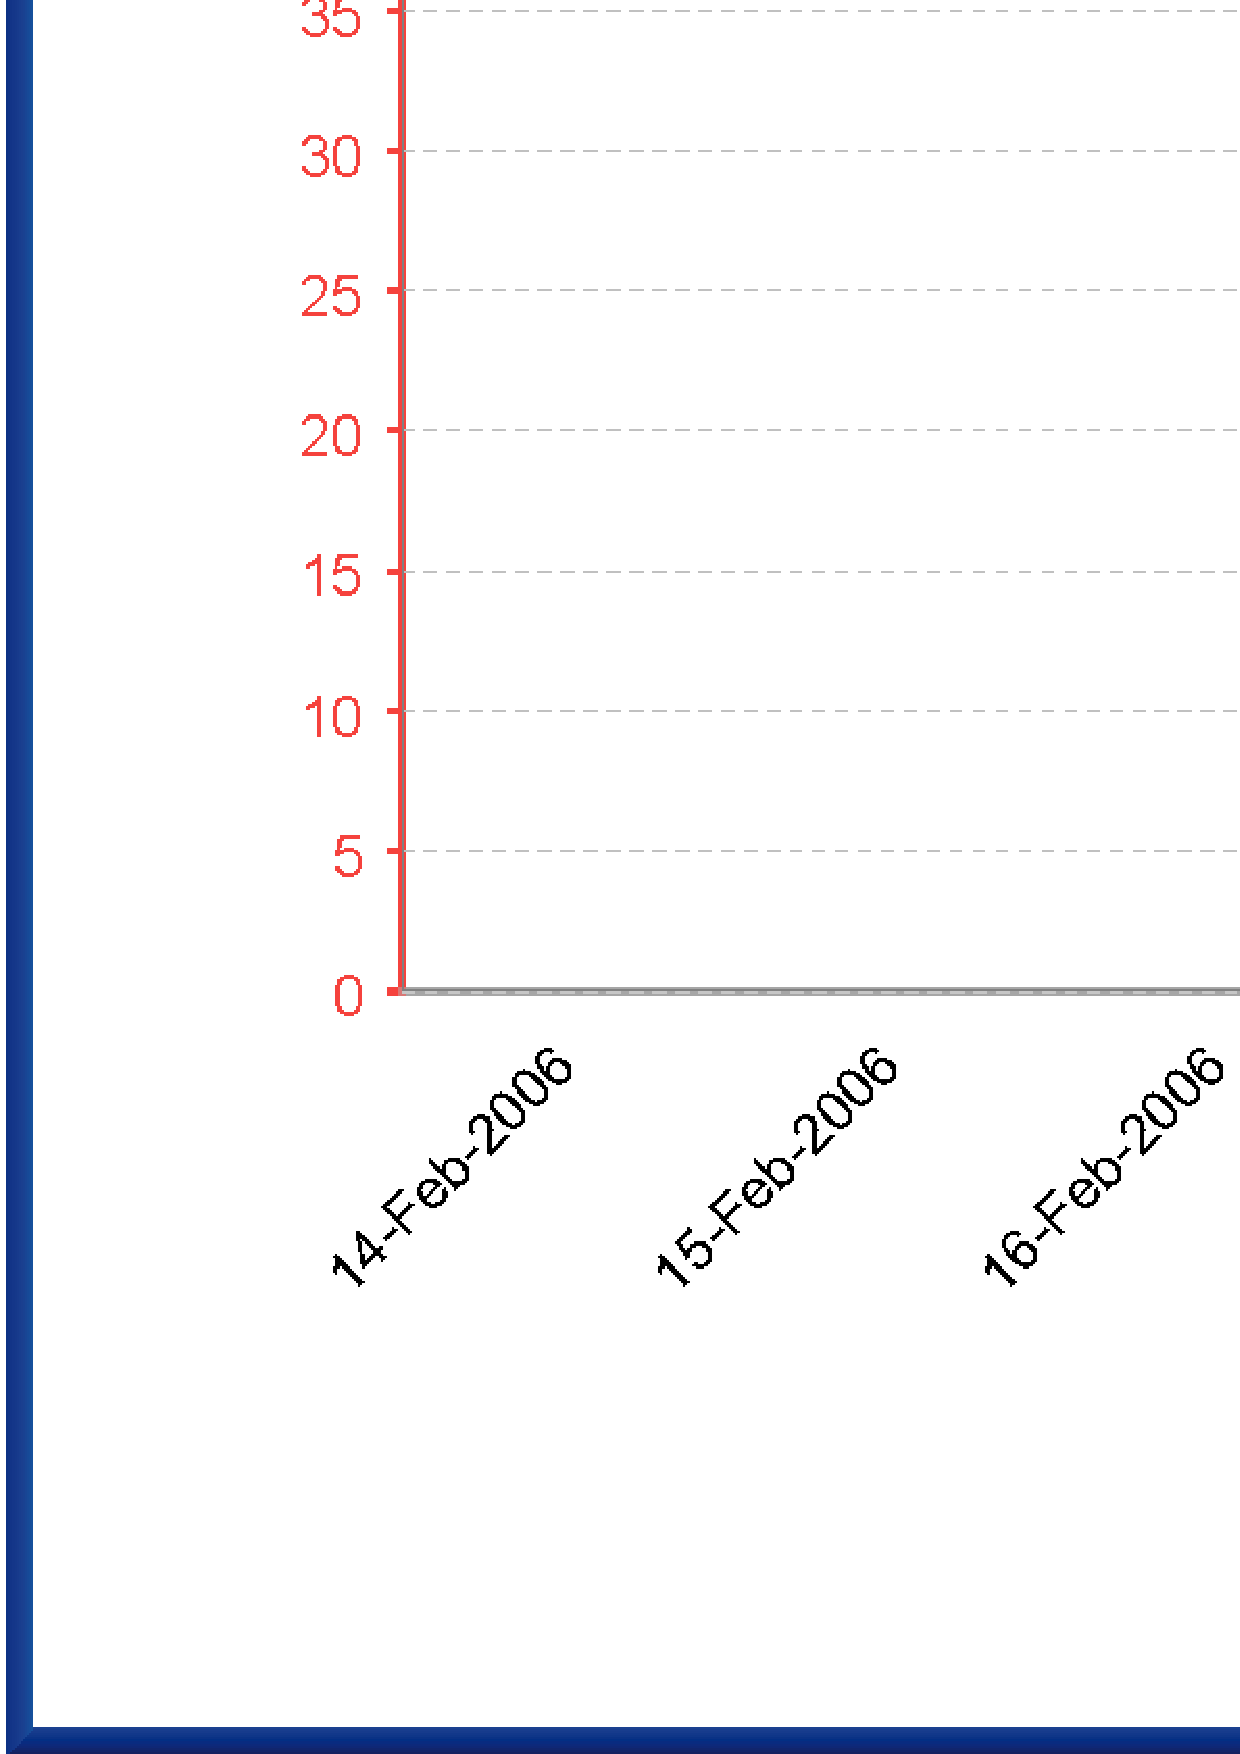
\includegraphics[width=0.70\textwidth]{figures/CSDL-CoverageSensorVerification}
  \caption{Telemetry Chart Indicating ``Emma'' Sensor not Working} 
  \label{fig:CSDL-CoverageSensorVerification}
\end{figure}

\begin{figure}[p]
  \center
  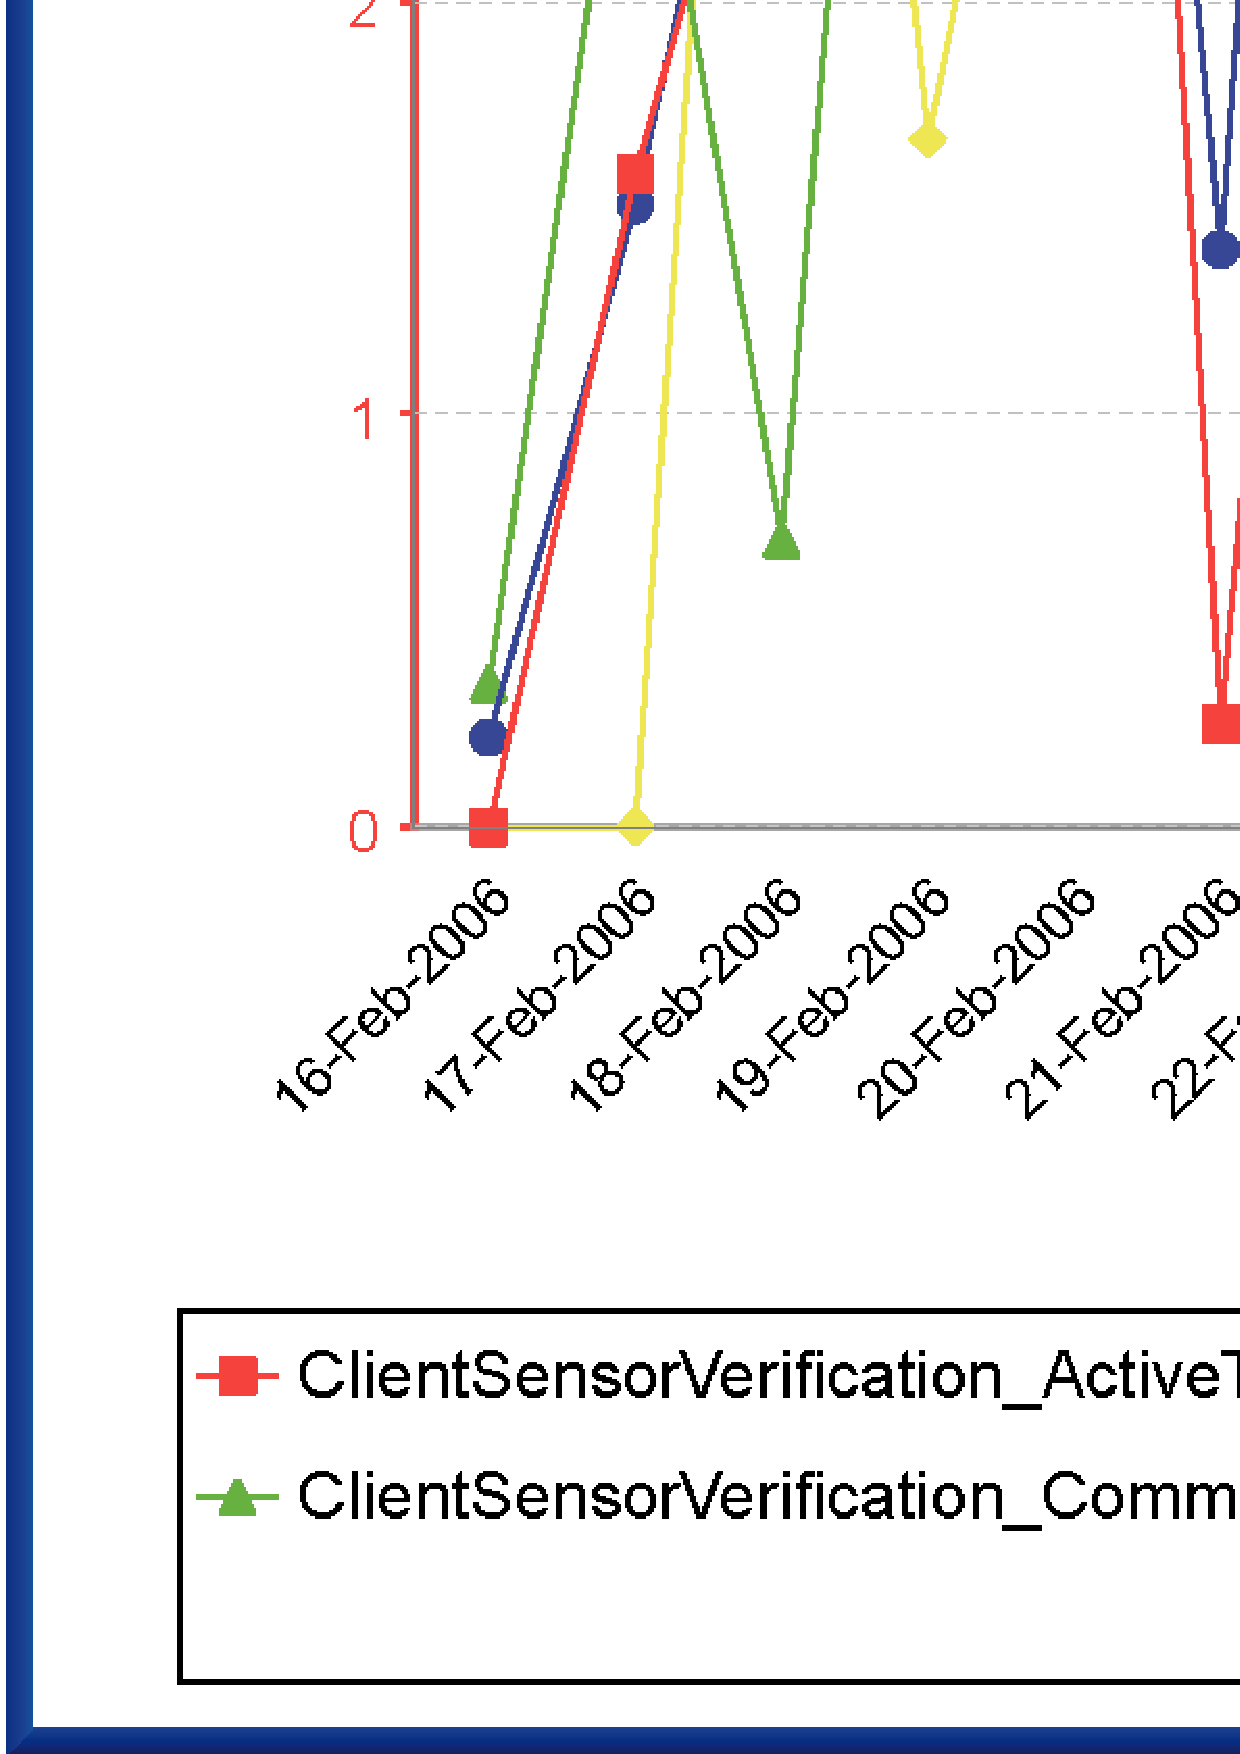
\includegraphics[width=0.70\textwidth]{figures/CSDL-DeveloperSensorVerification}
  \caption{Telemetry Chart Indicating ``Eclipse'' Sensor not Working} 
  \label{fig:CSDL-DeveloperSensorVerification}
\end{figure}











%%%%%%%%%%%%%%%
%  S T O R Y  %
%%%%%%%%%%%%%%%
\clearpage
%\subsection{Software project telemetry will not likely to provide value where low-level details are needed.} 
\subsection{Limitation on Low-level Details}
\label{EvaluationInCSDL:EventsDescription:Limitation}

\subsubsection{Pre-hypothesis Data:}
\begin{itemize}
  \setlength{\itemsep}{0pt}
  \setlength{\parskip}{0pt}
  \item 2006-02-05-1: I designed telemetry charts for the telemetry wall. Some of the charts were devoted to project level and individual level release cycle issue tracking. 
  \item 2006-02-06-1: I introduced the telemetry wall in the weekly status meeting. While the project level issue tracking charts were found \textit{``highly useful''} by the project manager, the individual level issue tracking charts were completely useless. One developer commented: \textit{``I would rather look into \textit{Jira} directly, because I don't know which issues remain.''} The project manager commented: \textit{``I would not be interested in those individual charts.''}
\end{itemize}

\subsubsection{Generated Hypothesis:}

The plausible explanation was related to information abstraction. Telemetry analyses offer high level perspectives on software development process by discarding low level details. The project manager's job was to make sure progress has been made and the software can be released as scheduled. He did not have to know low level details about individual issue. Project level issue tracking charts had the right level of abstraction to help him make release cycle decisions. On the other hand, the developers had to know issue details in order to fix them, but such information had already been discarded by telemetry analyses. 

\subsubsection{Intervention:}

None, except that I removed the individual level issue tracking charts from the telemetry wall.

\subsubsection{Post-hypothesis Data:}
\begin{itemize}
  \setlength{\itemsep}{0pt}
  \setlength{\parskip}{0pt}
  \item 2006-04-25-1: I modified the code issue telemetry chart to track the number of warnings falling into ``fail'' and ``monitor'' categories. The chart was primarily designed to be used by the project manager. I enhanced FindBugs report. Warnings in the ``fail'' category were highlighted in red color, and warnings in the ``monitor'' category were highlighted in blue color. I also modified the build script so that the developers could generate the report with single command on their workstations. This was primarily designed to be used by the developers to fix the warnings.
  \item 2006-05-06-1: Telemetry analysis indicated that all FindBugs warnings in the ``fail'' category had been eliminated. I had not received any complaint from the developers about the enhanced FindBugs report.
\end{itemize}

\subsubsection{Conclusion:}

The post-hypothesis data indicated that I had learned my lesson about information abstraction in telemetry analyses. Apart from the code issue tracking charts, I provided enhanced FindBugs report to supply low level details necessary for the developers to eliminate the potential bugs.
Both the issue tracking experience and the FindBugs experience seem to suggest that telemetry analyses will likely to provide decision-making value when a task requires relatively high level information abstraction, but they will not likely to provide value for tasks that require low level details.

\subsubsection{Elaboration:}

%This subsection reports on a failed attempt to use \textit{software project telemetry} to help an individual developer track \textit{``Jira''} issues assigned to him. 

At the early stage of this study, two of the scenes on the telemetry wall were related to release cycle issue tracking. One of them contained charts for project level issue tracking, while the other contained charts for individual level issue tracking. 
Figure \ref{fig:CSDL-Issue730} and \ref{fig:CSDL-Issue740} were two examples of project level issue tracking charts. The charts were a huge success with the project manager (see Section \ref{EvaluationInCSDL:EventsDescription:ProjectIssueTracking}), because they not only enabled him to track progress within each release cycle, but also established a baseline for future release cycle planning and scheduling.
The individual level issue tracking charts were similar to those for project level issue tracking. The only difference was that the individual issue tracking charts were developer-specific, and telemetry streams they contained represented the number of issues assigned to that specific developer instead of all the issues in the project. I provided each developer an individual issue tracking chart, intending to help him manage his assigned issues. However, the developers found the charts useless, and one of them commented: \textit{``I would rather look into Jira (the issue tracking database) directly, because I don't know which issues remain.''} The project manager found the charts useless too, and he commented: \textit{``I would not be interested in those individual charts.''}  

This was very interesting phenomenon. The project level issue tracking charts did not differ too much from the individual level charts. However, the former were found highly useful while the latter completely useless. 

My hypothesis was related to information abstraction. Telemetry analyses offer high level perspectives on software development. In other words, the analyses discard low level details. In case of release cycle issue tracking, the project manager's job is to make sure progress has been made and the software can be released as scheduled. He does not have to know about the details of each issue. The project level issue tracking charts offer the right level of abstraction to help him to make project management decisions. On the other hand, the developers' job is to resolve issues. They have to know the details about each issue, which means they have to delve into the issue tracking database to find the information. Besides, the CSDL developers usually have only 3 to 10 open issues to track at any moment. The abstraction in the individual issue tracking charts does not provide any value to them.

As a result, when I helped CSDL improve the utilization of ``CodeIssue'' metrics and FindBugs reports (see Section \ref{EvaluationInCSDL:EventsDescription:CodeIssue}), I learned from my previous experience. I used two sets of intervention procedures targeting the project manager and the developers separately. On the manager side, I provided a telemetry chart (see Figure \ref{fig:CSDL-FindBugs}) showing the number of FindBugs warning in \textit{``fail''} and \textit{``monitor''} categories respectively. The chart was monitored by the project manager as one of the project quality indicators. On the developers' side, I enhanced the original FindBugs report. Warnings in the \textit{``fail''} category were highlighted in red color, and warnings in the \textit{``monitor''} category were highlighted in blue color. For each reported potential bug, the enhanced report not only told the developers the category it belonged to, but also pinpointed the location in the source code from which it was generated.

The FindBugs experience appears to confirm the hypothesis. Both the issue tracking and the FindBugs experiences seem to suggest that telemetry analyses will likely to provide decision-making value when a task requires relatively high level information abstraction, such as project macro-management and high level process analysis. One the other hand, telemetry analyses will not likely to provide value for tasks that require low level details, such as resolving issues and fixing bugs.


\begin{figure}[tbp]
  \center
  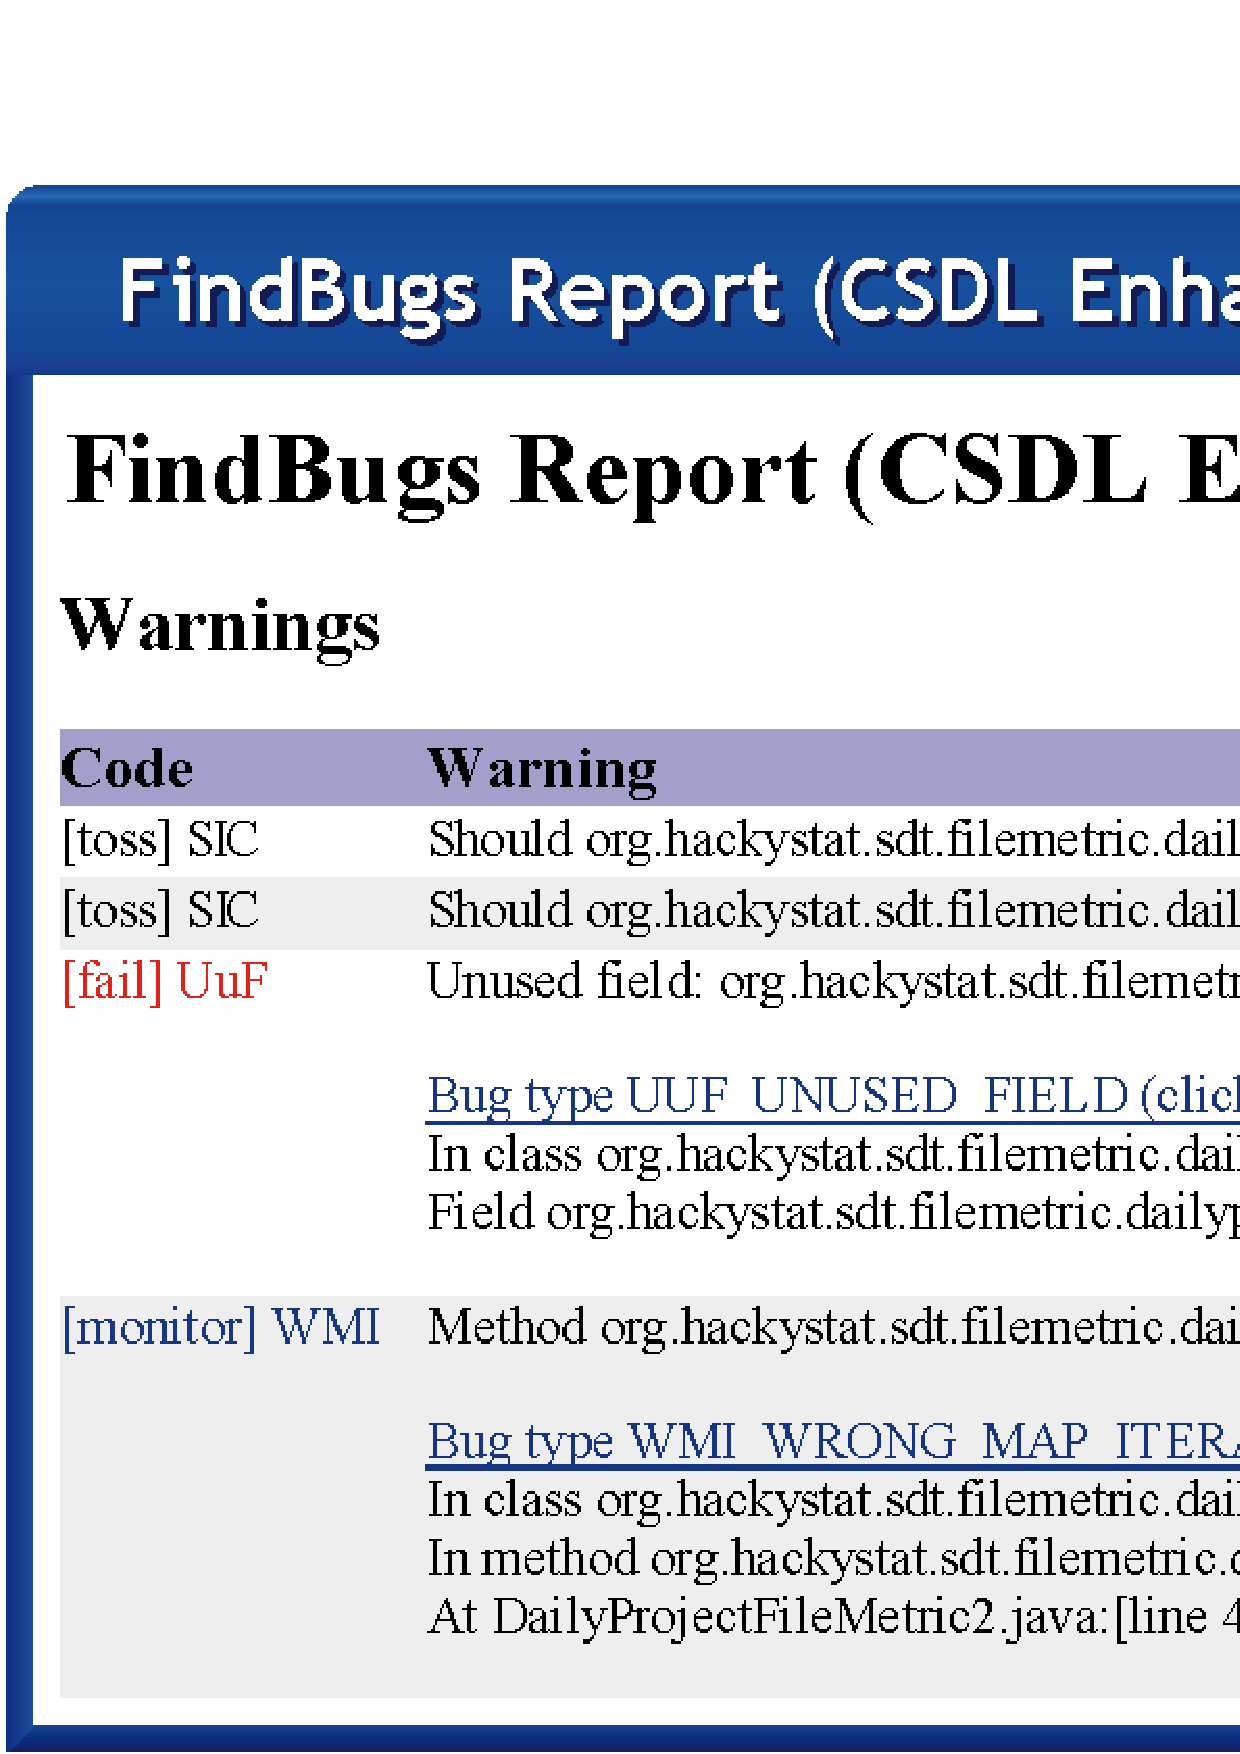
\includegraphics[width=1.00\textwidth]{figures/CSDL-FindBugsReport}
  \caption{CSDL Enhanced Version of FindBugs Report} 
  \label{fig:CSDL-FindBugsReport}
\end{figure}




%%%%%%%%%%%%%%%
%  S T O R Y  %
%%%%%%%%%%%%%%%
\clearpage
%\subsection{I enhanced the telemetry language with filter functions.} 
\subsection{Telemetry Language Enhancement with Filter Functions}
\label{EvaluationInCSDL:EventsDescription:FilterFunction}

\subsubsection{Pre-hypothesis Data:}
\begin{itemize}
  \setlength{\itemsep}{0pt}
  \setlength{\parskip}{0pt}
    \item 2006-02-20-1: While redesigning telemetry charts for the telemetry wall, I noticed several charts for module-level telemetry trends were overly cluttered (e.g., Figure \ref{fig:CSDL-UnfilteredCoverage}).
    \item 2006-02-21-2: I discussed the charts with three developers. They commented that those charts were too cluttered to be useful. One of them also noted that most of the lines were ``uninteresting'' because they represented inactive modules.
\end{itemize}

\subsubsection{Generated Hypothesis:}

The telemetry language could be enhanced with filter functions to filter out ``uninteresting'' telemetry streams. This could solve the usability and scalability problem with telemetry charts for large projects.  

\subsubsection{Intervention:}

I augmented the telemetry language to support nested function calls, and implemented special-purpose functions to support filtering telemetry streams in various ways.

\subsubsection{Post-hypothesis Data:}
\begin{itemize}
  \setlength{\itemsep}{0pt}
  \setlength{\parskip}{0pt}
  \item 2006-03-15-5: In an email request for comments, I brought up the idea of introducing nested function calls to the telemetry language.
  \item 2006-03-16-2: A Jira issue (HACK-612) was created to solve the usability and scalability problem of telemetry charts for large projects.
  \item 2006-03-17-2: The project manager used the telemetry wall to show the status of Hackystat development to outsider developers. For those overly-cluttered charts, he had to enlarge them to occupy all the nine screens to show the details.
%  \item 2006-03-17: I held a discussion with the project manager. We reached the consensus to implement filter functions as a special case of my recently proposed nested function calls.
  \item 2006-04-09-1: I finished the implementation of filter functions and closed the Jira issue (HACK-612).
  \item 2006-04-11-1: I revised the module-level coverage charts on the telemetry wall by applying filters to show only the top 5 and bottom 5 covered modules (e.g., Figure \ref{fig:CSDL-FilteredCoverage}). The developers liked the changes, but they requested a chart to show modules with coverage that changed most.
  \item 2006-04-17-4: I revised the filter function implantation, and made the chart showing modules with coverage that changed most available on the telemetry wall. One of the developers commented that filter functions made the chart not only much cleaner but also much useful. 
\end{itemize}

\subsubsection{Conclusion:}

The filter function is a useful enhancement to the telemetry language. It appeared to solve the usability and scalability problem with telemetry charts for large projects. 

\subsubsection{Elaboration:}

The initial telemetry language had only reduction functions, which take sensor data as input and output one or more telemetry streams. In the CSDL study, I noticed a significant usability and scalability challenge with telemetry charts to present ``interesting'' information from a large number of streams. For a large project, simple telemetry definitions could easily produce charts cluttered with dozens or even hundreds of lines. For example, Hackystat had over 70 modules, one frequent use of software project telemetry was to compare the values and trends of metrics between different modules. One of the charts on the telemetry wall used the following definition to present an overview of module-level test coverage in the Hackystat source: 

\begin{verbatim}
      y-axis yAxis(label) = {
        label, "integer", 0, 100
      };

      streams ModuleCoverageStreams() = {
        "Coverage by Modules",
        WorkspaceCoverage("Percentage", "**", "line")
      };

      chart ModuleCoverageChart() = {
        "Unit Test Coverage by Modules",
        (ModuleCoverageStreams(), yAxis("Percent"))
      };

      draw ModuleCoverageChart();
\end{verbatim}

It generated one telemetry stream for each individual module in the project. The resulting chart was shown in Figure \ref{fig:CSDL-UnfilteredCoverage}. It contained over 70 lines, which created a severe usability problem. Discussion with the developers revealed that they generally were only interested in a small subset of those lines, such as the modules with highest or lowest coverage or the modules with coverage that changed most. But it was overwhelming to locate such information in a chart cluttered with over 70 lines. 
%The developers wished there could be an automated mechanism to help them sift through the large amount of information. 

My hypothesis was that filter functions could be added to the telemetry language to filter out ``uninteresting'' telemetry streams, which could solve the usability and scalability problem with telemetry charts for large projects. Based on this hypothesis, I augmented the telemetry language to support nested function calls, and implemented special-purpose functions to support filtering telemetry streams in various ways.

The following example illustrated the use of two filter functions:

\begin{verbatim}
      streams ModuleCoverageStreams() = {
        "Coverage by Modules",
        Filter(
            FilterZero(
                WorkspaceCoverage("Percentage", "**", "line")
            ), "SimpleDelta", "Bottom", 3
        )
      };
\end{verbatim}

Both \textit{``Filter''} and \textit{``FilterZero''} were the name of filter functions. They were invoked on the stream expression for test coverage for all modules. In other words, the input to the filter functions was the output from the \textit{``WorkspaceCoverage''} reduction function, which was visually represented in Figure \ref{fig:CSDL-UnfilteredCoverage}. The \textit{``FilterZero''} function got rid of all lines with only zero values, while the \textit{``Filter''} function further reduced the set of telemetry lines to the three with the most significant decrease in value during the interval. The effect was to produce a chart showing the modules that were decreasing the most in test coverage. The resulting chart was illustrated in Figure \ref{fig:CSDL-FilteredCoverage}. It contained the modules potentially most in need of additional quality assurance resources.

\begin{figure}[p]
  \center
  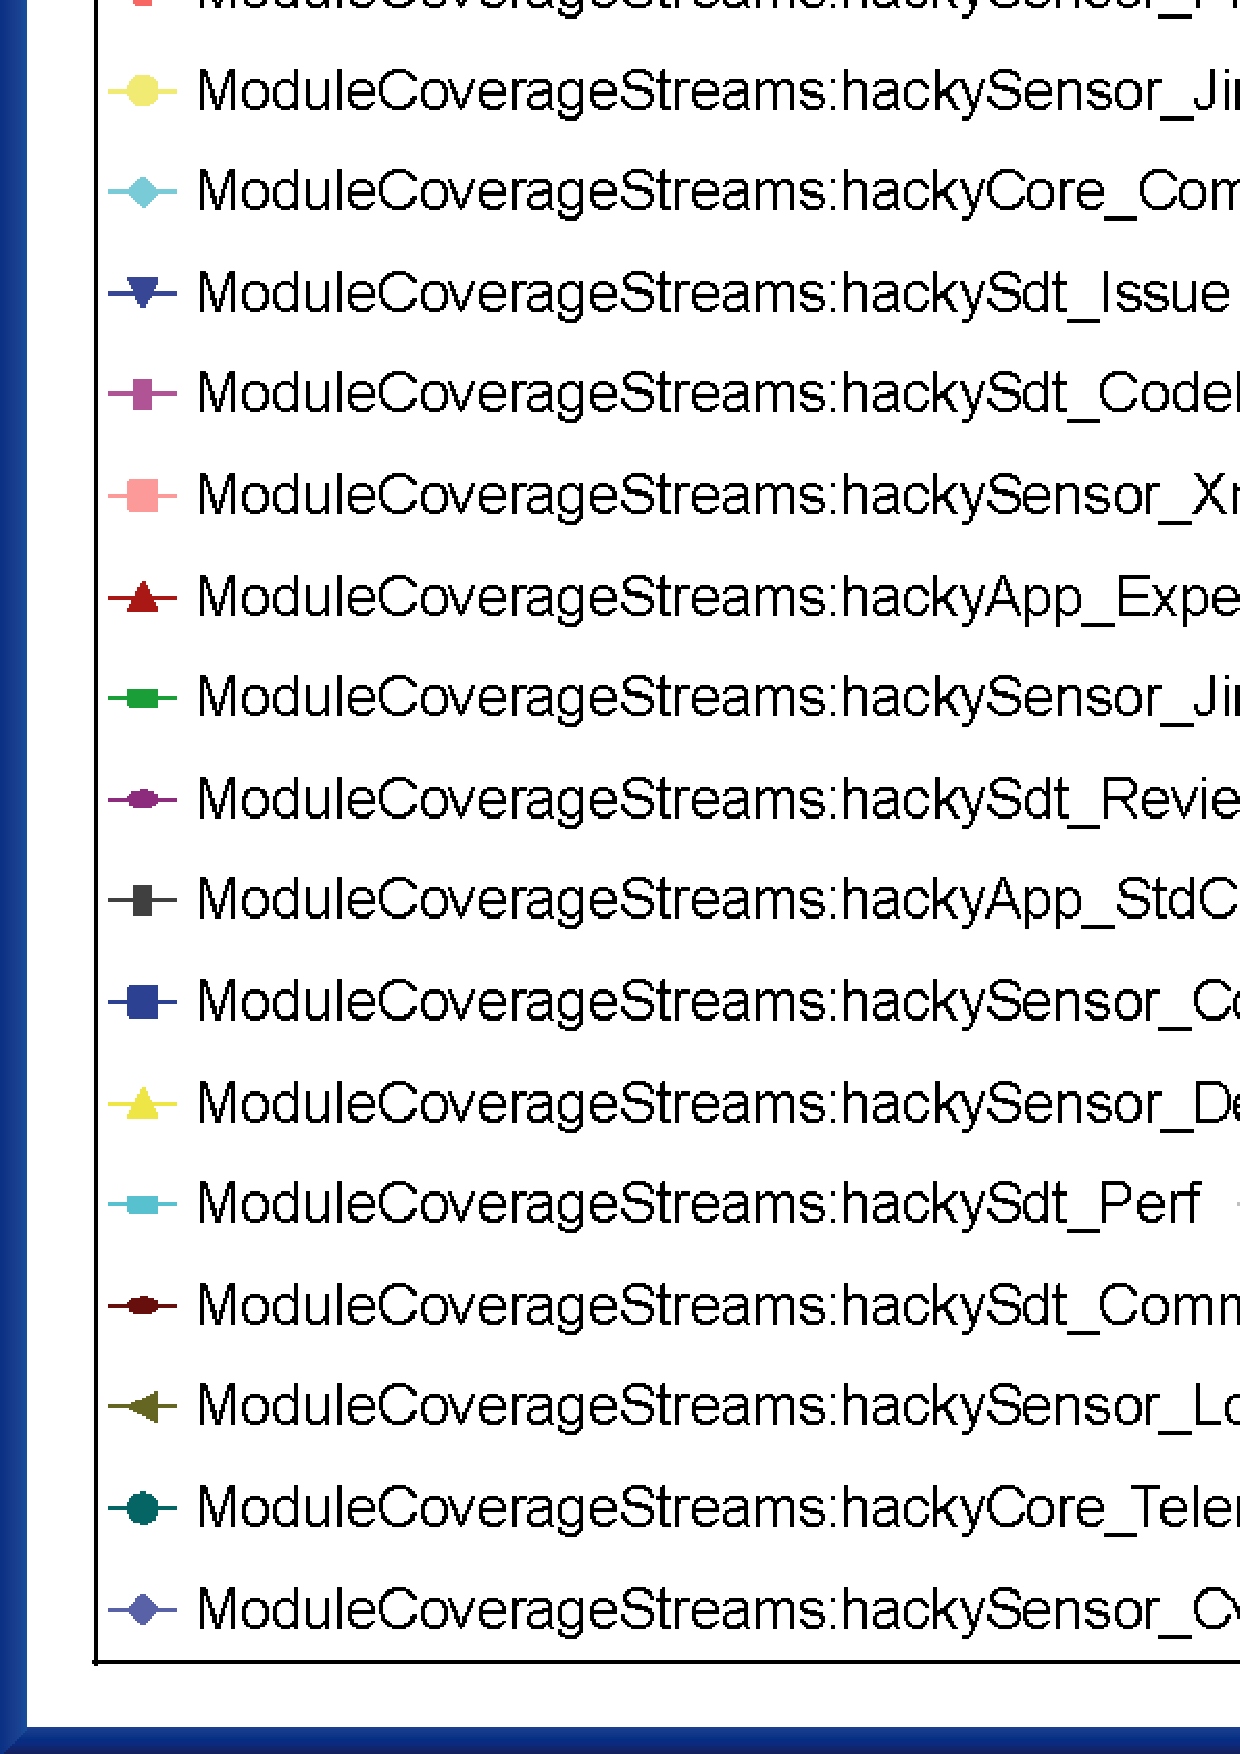
\includegraphics[height=0.93\textheight]{figures/CSDL-UnfilteredCoverage}
  \caption{Telemetry Chart with Unfiltered Module Coverage} 
  \label{fig:CSDL-UnfilteredCoverage}
\end{figure}

\begin{figure}[p]
  \center
  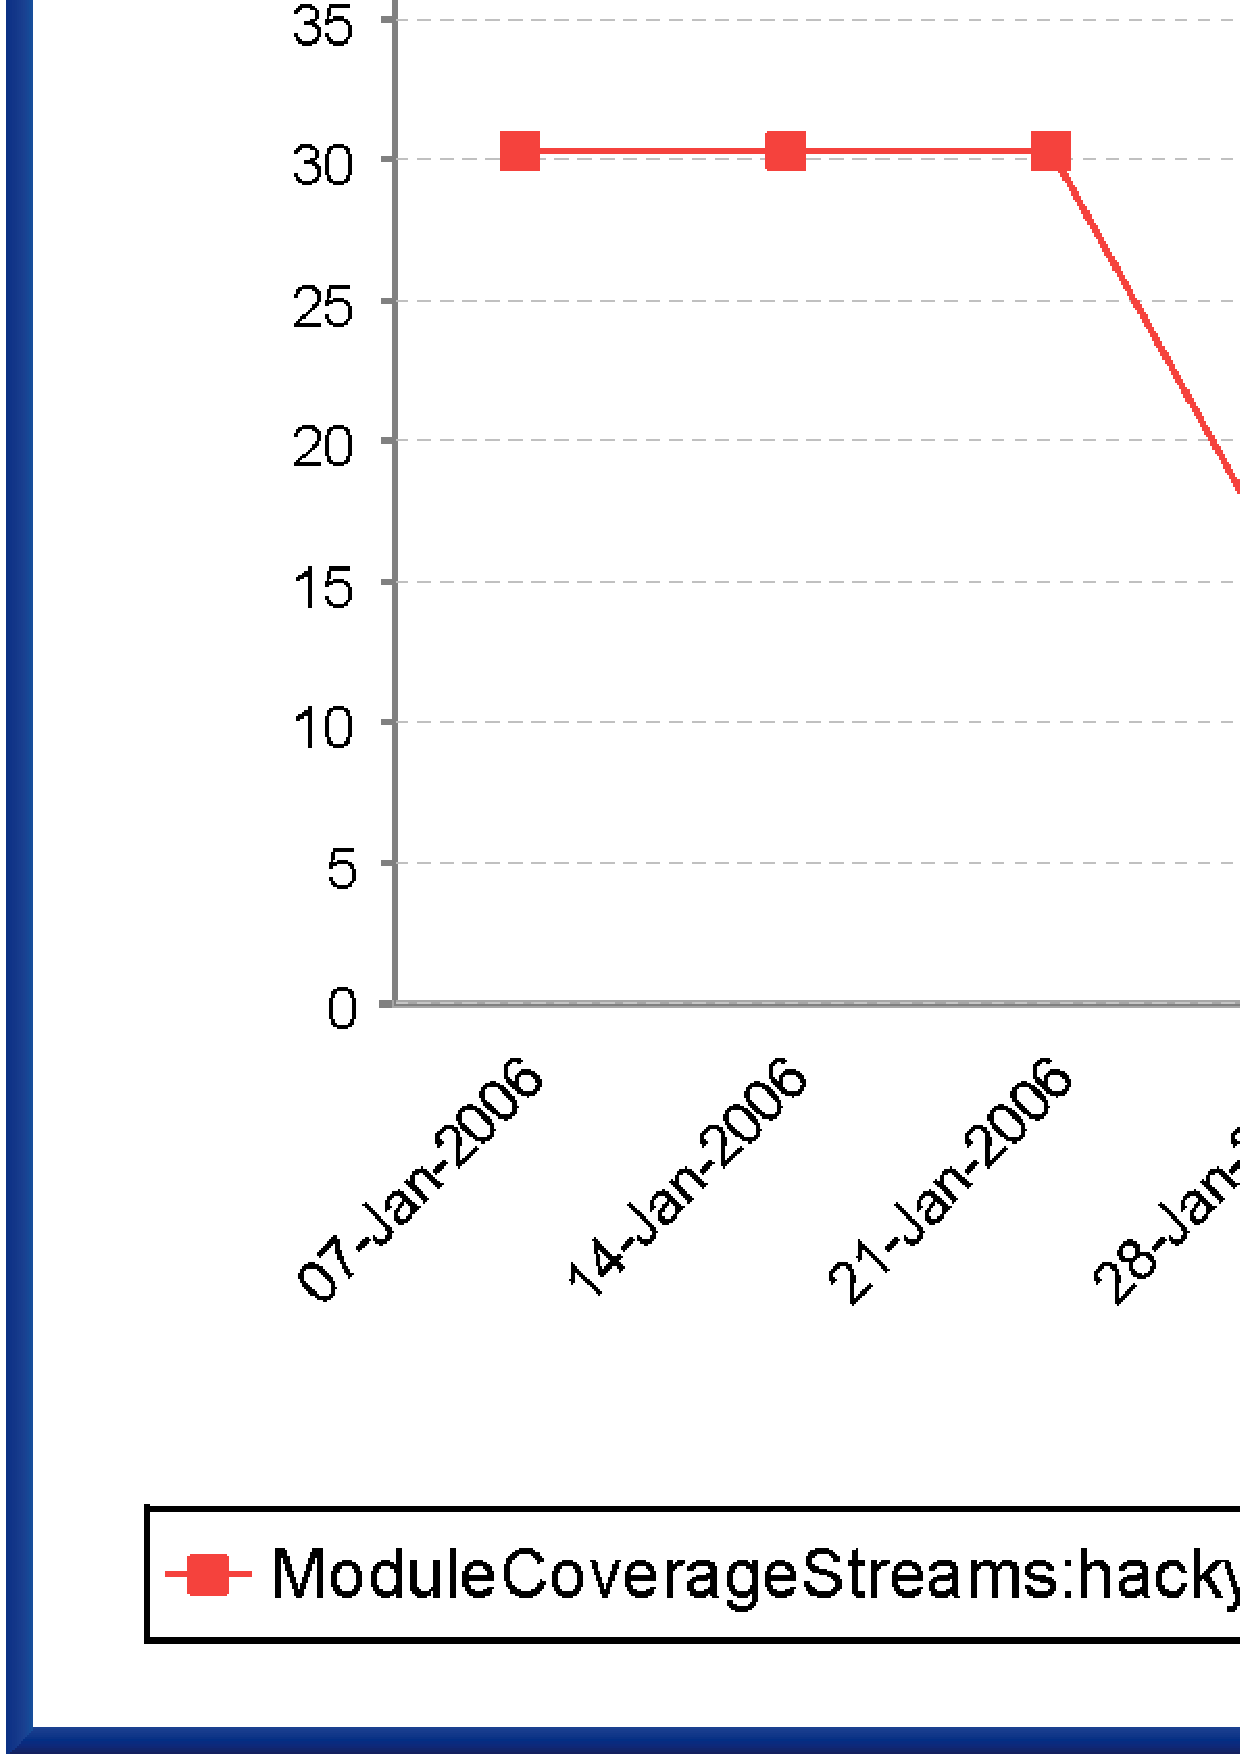
\includegraphics[width=0.70\textwidth]{figures/CSDL-FilteredCoverage}
  \caption{Telemetry Chart with Filtered Module Coverage} 
  \label{fig:CSDL-FilteredCoverage}
\end{figure}













%%%%%%%%%%%%%%%
%  S T O R Y  %
%%%%%%%%%%%%%%%
\clearpage
%\subsection{I enhanced the telemetry language with y-axis construct.} 
\subsection{Telemetry Language Enhancement with Y-axis Construct}
\label{EvaluationInCSDL:EventsDescription:VerticalAxis}

\subsubsection{Pre-hypothesis Data:}
\begin{itemize}
  \setlength{\itemsep}{0pt}
  \setlength{\parskip}{0pt}
  \item 2006-02-02-2: I showed some module level coverage charts to a developer. He noted that the automatically-scaled y-axis made comparison across related charts difficult.
  \item 2006-02-22-1: I discussed the module level quality indicator telemetry scene with the project manager. We had to check the vertical axis while comparing coverage trends in different modules.  
\end{itemize}

\subsubsection{Generated Hypothesis:}

It would be useful to allow a user to have the option to explicitly specify the range of the vertical axis in a telemetry chart. This way, related charts could be made more comparable by making them have the same vertical axis. The benefit of this extra level of control would outweigh the slight complexity it added to the telemetry language.

\subsubsection{Intervention:}

I augmented the telemetry language by adding \textit{``y-axis''} construct.

\subsubsection{Post-hypothesis Data:}
\begin{itemize}
  \setlength{\itemsep}{0pt}
  \setlength{\parskip}{0pt}
  \item 2006-03-16-1: During a discussion of telemetry charts with the project manager, I mentioned the idea of making relating charts more comparable by augmenting the telemetry language to allow a user to specify the vertical axis manually. He agreed that it would improve the usability of telemetry charts. 
  \item 2006-03-17-3: A Jira issue (HACK-616) was created to enhance the telemetry language to allow manually specified vertical axis.
  \item 2006-04-03-1: I held a discussion with the project manager, and we formalized the change to the telemetry language in order to allow a user to specify the vertical axis manually.
  \item 2006-04-09-2: I enhanced the telemetry language with \textit{``y-axis''} construct, and closed the Jira issue (HACK-616). 
  \item 2006-04-11-1: I update the telemetry wall, converting some charts to use manually-specified y-axises. I showed the changes to the project manager and the developers. They thought the change had improved the usability a lot, because comparisons could be made more intuitively with fixed vertical axises. 
\end{itemize}

\subsubsection{Conclusion:}

The user feedback after I enhanced the telemetry language with \textit{``y-axis''} construct suggested that it was a useful feature.

\subsubsection{Elaboration:}

%The telemetry wall is designed to display multiple telemetry charts simultaneously. The idea is to allow easy comparison of telemetry trends in related charts. For example, the developers might use the telemetry wall to compare test coverage in different modules. 

The telemetry language is designed to be as simple as possible. Most aspects of telemetry presentation are automated, so that a user does not have to fiddle with minute details such as fonts, colors, and layouts. The original language did not have a construct to allow a user to manually specify the range of the vertical axis in a telemetry chart. Instead, it was automatically determined based on the values of the telemetry data points. The result was a simpler language, but, at the same time, different charts might have different value ranges on their vertical axises. This approach worked well in most cases, especially when the range of telemetry data values could not be estimated in advance. However, in the CSDL study, I discovered that it also caused some inconvenience with some charts. For example, Figure \ref{fig:CSDL-AutoYAxis} was generated using definitions written in the original language:

\begin{verbatim}
      streams CoverageStreams(filePattern) = {
        "Coverage",
        JavaCoverage("Percentage", filePattern, "line")
      };

      chart CoverageChart(filePattern) = {
        "Unit Test Coverage",
        (CoverageStreams(filePattern))
      };
\end{verbatim}

The two charts showed test coverage for two different modules in the Hackystat source. By cursory examination, you might conclude that coverage in the two modules did not differ too much. However, if you paid attention to the vertical axises, your conclusion would be very different: the module \textit{``hackyApp\_Zorro''} had significantly higher coverage than \textit{``hackyApp\_PrjSize''}. Though the utility of the charts was not affected, it was a usability issue nevertheless, and the developers pointed out that the automatically-scaled vertical axises made comparison across charts difficult for such cases.

My hypothesis was that it would be useful to allow a user to have the option to explicitly specify the range of the vertical axis in a telemetry chart so that related charts could be made more comparable, and that the benefit of this extra level of control would outweigh the slight complexity it added to the telemetry language. As a result, I augmented the telemetry language with \textit{``y-axis''} construct, whose syntax takes the following form:

\begin{verbatim}
      y-axis <YAxisName> <ParameterList> = { 
          <Label>, <NumberType> (, <LowerBound>, <UpperBound>)?
      };
\end{verbatim}

\textit{`LowerBound`} and \textit{``UpperBound''} are optional fields. A user can choose to provide values to these optional fields to explicitly specify the vertical axis range. Otherwise, the range is determined automatically. With the new \textit{``y-axis''} construct, the telemetry definitions in the previous example have to be updated to a slightly complex form:

\begin{verbatim}
      y-axis yAxis(label) = {
        label, "integer", 0, 100
      };

      streams CoverageStreams(filePattern) = {
        "Coverage",
        JavaCoverage("Percentage", filePattern, "line")
      };

      chart CoverageChart(filePattern) = {
        "Unit Test Coverage",
        (CoverageStreams(filePattern), yAxis("Percent"))
      };
\end{verbatim}

The result was demonstrated in Figure \ref{fig:CSDL-FixedYAxis}, which showed the same coverage information for the same two Hackystat modules as in Figure \ref{fig:CSDL-AutoYAxis}. But this time the vertical axises in the two charts had the same range from 0 to 100. The difference in coverage for the two modules in Figure \ref{fig:CSDL-FixedYAxis} was obvious, and the comparison could be made more intuitively. The developers welcomed the changes.

\begin{figure}[p]
  \center
  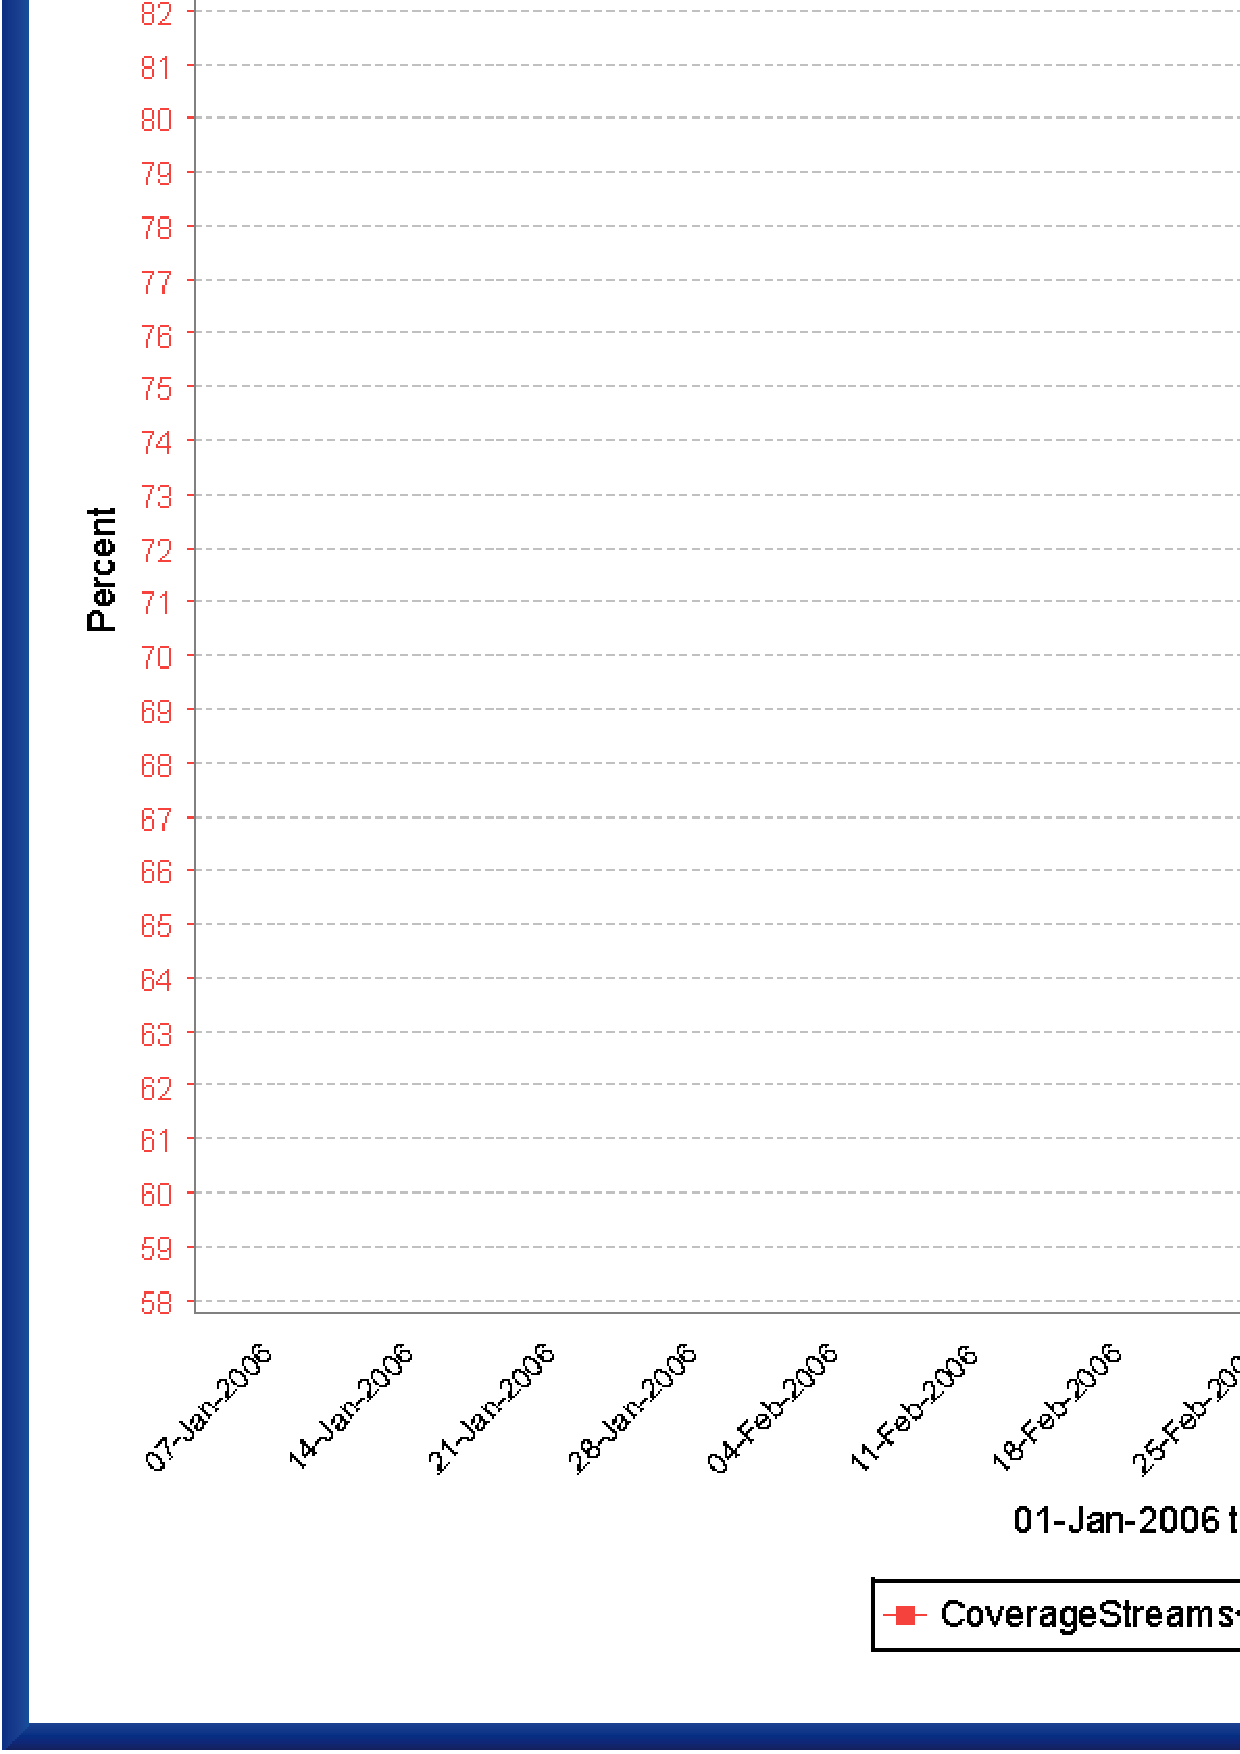
\includegraphics[width=1.00\textwidth]{figures/CSDL-AutoYAxis}
  \caption{Telemetry Charts with Automatically-scaled Vertical Axises} 
  \label{fig:CSDL-AutoYAxis}
\end{figure}

\begin{figure}[p]
  \center
  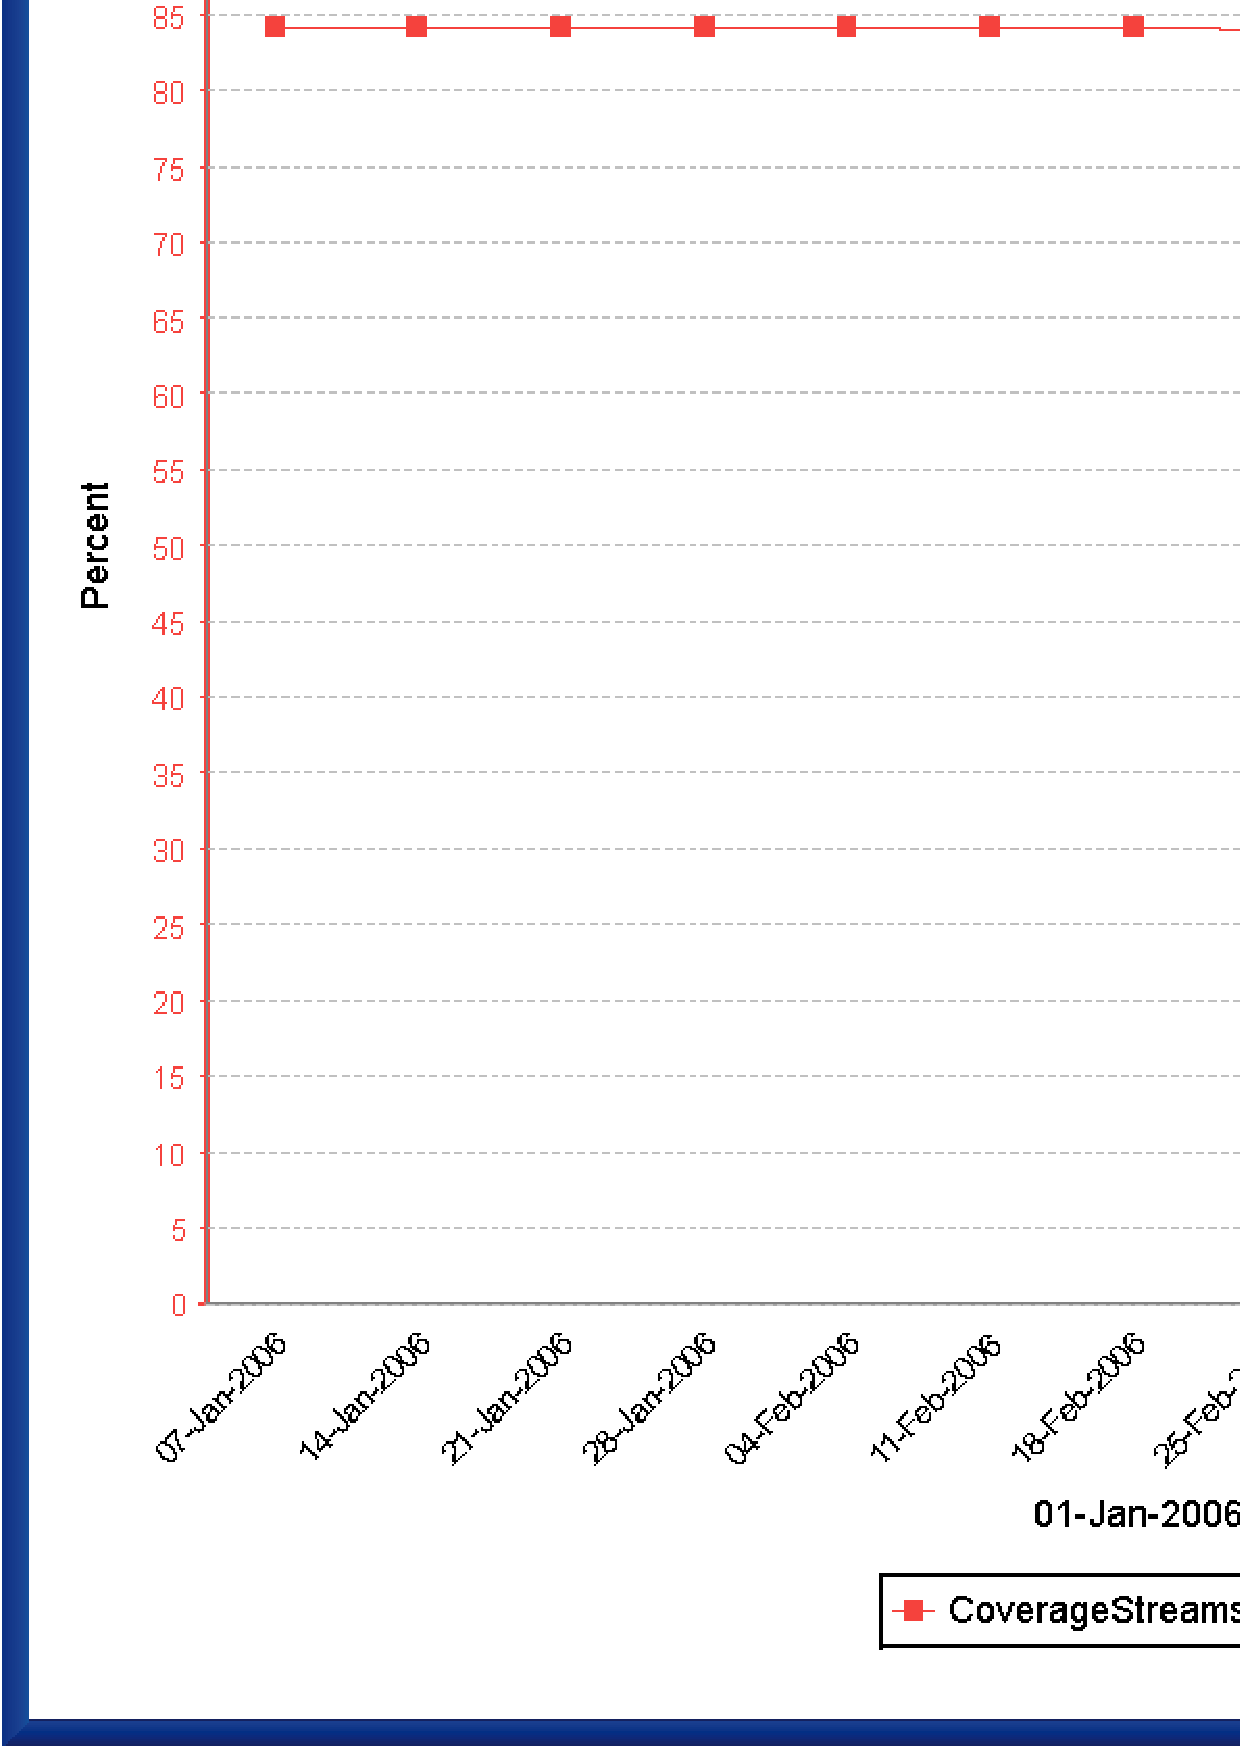
\includegraphics[width=1.00\textwidth]{figures/CSDL-FixedYAxis}
  \caption{Telemetry Charts with Manually-specified Vertical Axises} 
  \label{fig:CSDL-FixedYAxis}
\end{figure}



%%%%%%%%%%%%%%%
%  S T O R Y  %
%%%%%%%%%%%%%%%
%\subsection{G: It's Better to Hide the Telemetry Language from a Normal User.}








%%%%%%%%%%%%%%%
%  S T O R Y  %
%%%%%%%%%%%%%%%
\clearpage
%\subsection{I improved telemetry analysis runtime performance.}
\subsection{Runtime Performance Enhancement}
\label{EvaluationInCSDL:EventsDescription:Performance}

\subsubsection{Pre-hypothesis Data:}
\begin{itemize}
  \setlength{\itemsep}{0pt}
  \setlength{\parskip}{0pt}
  \item 2006-02-06-1: I demonstrated the telemetry wall in the weekly status meeting, and noticed that some of the charts covering long-term metrics trends could take several minutes to show up, which was more than the developers were willing to wait.
  \item 2006-02-13-2: I wanted to display some telemetry charts on the telemetry wall in the middle of the weekly status meeting, but encountered severe server timeout.
  \item 2006-02-23-1: One of the developers toggled the telemetry wall in auto-update mode. The server stopped responding under the heavy load, and its CPU usage stayed at 100\%. I had to restart the server.
\end{itemize}

\subsubsection{Generated Hypothesis:}

The performance problem was caused by the bottleneck in the data persistence layer, which used XML files to store sensor data. Given that machine processing of XML data was slow, the solution was to retain as many as possible the most often used sensor data instances in the cache.

\subsubsection{Intervention:}

I reviewed the code that interfered with the management of the sensor data cache, such as higher level user code not releasing references to sensor data instances. I modified the code to ensure that all references were released promptly.

\subsubsection{Post-hypothesis Data:}
\begin{itemize}
  \setlength{\itemsep}{0pt}
  \setlength{\parskip}{0pt}
  \item 2006-03-01-1: I reviewed the ``DailyProjectCoverage'' code, and found it that it never released references to sensor data instances, which was temporary data structure as far as ``DailyProjectCoverage'' is concerned. 
  \item 2006-03-05-2: The project manager created a Jira issue, requesting me to perform an audit on all daily project code to ensure references to temporary data structures were released.
  \item 2006-03-10-1: I started the code audit, and found several classes followed the same design pattern of ``DailyProjectCoverage,'' failing to release temporary data structures.
  \item 2006-03-11-2: After I sent out my findings, the project manager elaborated the distinction between ``cache'' and ``temporary data structure'' in an email to call to the attention of all the developers. 
  \item 2006-03-14-1: The server performance improved after the ``temporary data structures'' were properly disposed, but the improvement was not significant enough to reduce the telemetry wall response time to an acceptable range. I profiled the code with another developer, and we had a number of surprising findings. (1) When sensor data were cached in memory, over 90\% of processor time was spent on string comparison in workspace code. The case-sensitive comparison was 10 times more expensive than case-insensitive comparison. (2) The sensor data evolution mechanism in some classes was implemented very inefficiently. For example, the ``FileMetric'' class spent 80\% of processor time in the ``recognizeData()'' method, even if the data were already stored in the newest format. (3) The cost of reading sensor data from XML files was negligible.

  \item 2005-03-15-3: I sent out an email to the developer mailing list reporting the performance profiling result.

  \item 2006-03-15-4: After reporting the performance profile findings, I received an email from a former developer. He had experimented with a Berkeley XML DB back-end and found no performance improvement at all.

  \item 2006-03-21-2: An external user, who managed his own server, reported degrading telemetry analysis performance proportional to server up-time. He had not picked up the recent fixes, but the problem reported was consistent with the effect of not releasing temporary data structure. 
  \item 2006-04-05-2: There was a performance complaint on the daily project details analysis.
  \item 2006-04-06-2: In an email, one of the developers noted that there were many redundant computations in the daily project details analysis.
%  \item 2006-04-06: I responded that the code in daily project classes was only optimized for telemetry analysis. The daily project analysis reused that code, but it had completely different data access pattern than the telemetry analysis.
  \item 2006-04-07-2: One of the developers modified the ``DailyProjectUnitTest'' code taking advantage of its data access locality, and the result was remarkable: the analysis time for 2006-04-05 unit test metrics was reduced from 124 seconds to 6 seconds.
  \item 2006-04-10-1: I did the same thing with the ``DailyProjectFileMetric'' code, and reduced the analysis time for 2006-04-05 file metrics from 180 seconds to just 1 second.
  \item 2006-04-10-2: The project manager was happy with the results. He wanted to formally document the design pattern as a best practice in the Hackystat developer guide in the summer.
\end{itemize}

\subsubsection{Conclusion:}

The generated hypothesis was wrong. The performance problem was not caused by the XML data persistence layer. Instead, the main culprit was the excessive calls to the workspace comparison code.

\subsubsection{Elaboration:}

The metrics collected by the sensors contain very low level information. For example, a file size metric only captures the size information for one single file. However, telemetry analyses are performed at a much higher project level. They typically have to aggregate hundreds or thousands of metrics for a large project like Hackystat just to compute a telemetry data point representing one single day. Furthermore, analyses performed at the interval of weeks or months are usually produced by first computing a set of analysis at the daily grain size and then combining them together in some fashion to obtain the week or month value. Multiply that by the many different kinds of metrics on which telemetry analyses could be performed, and the fact that the telemetry wall sends multiple concurrent requests in order to display related charts simultaneously, the strain on the server resources could be easily overwhelming. 

At the beginning of this study, I found that the telemetry wall response was sluggish at best. It usually took more than several minutes for a telemetry scene to show up. I even experienced several incidents in which requests timed out and I had to restart the server to fix the problem. The sluggish performance caused a usability problem. You just cannot expect a user to push a button and then wait for several minutes for the result in an interactive situation.

Since software project telemetry was implemented as a Hackystat extension, the performance problem was intricately related to the Hackystat framework. The framework stores sensor data in XML files and uses extensive in-memory cache to improve system response time. My hypothesis for the performance problem was that it was caused by the bottleneck in the data persistence layer. Given that machine processing of XML data was slow, the solution was to retain as many as possible the most often used sensor data instances in the cache. Therefore, I started to look for code that interfered with the management of the sensor data cache, such as higher level user code not releasing references to sensor data instances. However, despite my effort of fixing the code, the performance improvement was not significant enough to reduce the telemetry wall response time to an acceptable range. I began to believe that there was no way to improve the performance except by adding more memory to the server.

The turning point was the day when I profiled the system with another developer. We had a number of surprising findings. We discovered that most processor time was spent on string comparison in workspace code. We also discovered inefficiencies introduced in the recent sensor data type enhancement. However, the most shocking discovery was that the persistence layer was not a bottleneck at all, because the profiler indicated that the time spent reading and parsing sensor data from XML files was negligible. Based on the findings, the code was reorganized to minimize the number of string comparison instead of XML file read. The result was dramatic. In the most significant case, the time computing 2006-04-05 file metrics for all modules in the \textit{Hackystat} project was reduced from 180 seconds to just one second. 

My hypothesis was wrong. It reflected the intuition on my part. Though it explained the observed fact in the pre-hypothesis data well, it was inconsistent with the post-hypothesis data. The performance problem was not caused by the XML data persistence layer at all. I learned an important lesson through this experience: application performance improvement should be always guided by profiling data instead of intuition.










%%%%%%%%%%%%%%%
%  S T O R Y  %
%%%%%%%%%%%%%%%
%\clearpage
%\subsection{An Experience of Empirically Resolving Some Metrics Contentions}
%\label{EvaluationInCSDL:Results:WhichMetrics}
%
%It's not uncommon in software metrics research and practice to see several definitions for a metrics. But, often time, there is not enough anecdotal evidence to support which definition of the metrics provides the best decision-making value. This subsection reports on my experience in CSDL to use \textit{software project telemetry} to empirically resolve such contentious problems for the \textit{Hackystat} project.
%
%For example, a former CSDL graduate student had developed a unit test coverage tool called \textit{``JBlanket''}\cite{Software:JBlanket}, which was subsequently adopted by the \textit{Hackystat} project. Since \textit{JBlanket} was only capable of computing \textit{method-level} coverage, the \textit{Hackystat} developers always wondered whether a more fine-grained criterion such as \textit{line-level} coverage would be a better indicator of code quality, and whether they should switch to a more-capable unit test coverage tool, such as Clover \cite{Software:Clover} and Emma \cite{Software:Emma}.
%
%The telemetry chart in Figure \ref{fig:CSDL-CoverageComparison} provides the empirical answer. It contains four telemetry streams about unit test coverage computed using four different criteria: \textit{class-level}, \textit{method-level}, \textit{block-level}, and \textit{line-level}. The chart indicates that though \textit{class-level} coverage might be too coarse-grained, there is no significant difference in the other three criteria except absolute values. As far as the \textit{Hackystat} project is concerned, the \textit{method-level} coverage provided by \textit{JBlank} has the same decision-making value as the more fine-grained \textit{line-level} coverage. Therefore, there is no need to replace \textit{JBlanket}.
%
%On a side note, CSDL did replaced \textit{JBlanket} with \textit{Emma} eventually. But the reason was a completely different one: \textit{JBlanket} was out of maintenance and incompatible with Java 5 byte code format.
%
%Another example was related to file size metrics. During the course of this study, CSDL developed an enhanced version of SCLC \cite{Software:SCLC}. It counts the size of 27 types of source code files, providing the number of comment, non-comment, blank, and total lines. CSDL used to use a size counting tool called LOCC \cite{Software:LOCC}. Compared to \textit{SCLC}, \textit{LOCC} only counts Java size, but it can count the number of methods and Java classes which \textit{SCLC} cannot. The \textit{Hackystat} developers wanted to replace \textit{LOCC} with \textit{SCLC}, but they were not sure whether the loss of capability to count the methods and Java classes would impair their metrics-based decision-making capability or not. \textcolor{red}{Philip Comment: Must be explicit about the observational data that exists to support this.}
%
%The telemetry chart in Figure \ref{fig:CSDL-SizeComparison} provides the empirical answer. It contains three telemetry streams about the \textit{Hackystat} project size: the number of Java classes, the number of methods, and the number of uncommented source lines. The chart indicates that there is no significant difference in the three counting rules except absolute values. Therefore, replacing \textit{LOCC} has no negative impact on CSDL metrics-based decision-making capability.
%
%\begin{figure}[p]
%  \center
%  \includegraphics[width=0.70\textwidth]{figures/CSDL-CoverageComparison}
%  \caption{Test Coverage Measured by Different Criteria} 
%  \label{fig:CSDL-CoverageComparison}
%\end{figure}
%
%\begin{figure}[p]
%  \center
%  \includegraphics[width=0.70\textwidth]{figures/CSDL-SizeComparison}
%  \caption{System Size Measured by Different Criteria} 
%  \label{fig:CSDL-SizeComparison}
%\end{figure}








%%%%%%%%%%%%%%%
%  S T O R Y  %
%%%%%%%%%%%%%%%
%\subsection{Unable to use some metrics, no decision-making value.}
%\label{EvaluationInCSDL:Results:UnableToUseSomeMetrics}

%This section reports two type of metrics that were collected in CSDL, but I 
%
%1. Performance metrics.
%
%The idea is quite simple: a telemetry for performance, if goes down, then we investigate.
%We were never able to use this metrics: (1) test case non-typical, (2) same machine, subject to variable, (3) Java, non-deterministic, if there is slow memory leak, short period of performance test not able to reveal it. (4) Too much technology stack: tomcat, jvm, os.  
%
%2. Java dependency.
%
%Idea: complexity of modules or package or class. If it exceed a threashold, then we can do something.
%not even know how to define complexity, at what level.
%related to maintainability. good in theoty. In reality, famililarity most important. Everyone think his own module is easiest to maintain. 
%
%Internal cohesion, external dependency: all relative concept. Not sure whether those metrics are validated or not.
%
%BUT we are still collecting the data: (1) ESTABLISH	a baseline, (2) might be useful in the future, like findbugs.








%%%%%%%%%%%%%%%
%  S T O R Y  %
%%%%%%%%%%%%%%%
%\subsection{De-emphasize active time}
%\label{EvaluationInCSDL:Results:DeemphasizeActiveTime}
%
%IDE-sensor collects internal buffer size change event, and active time are calculated based on those event.
%
%CSDL-developer: only find it interesting, don't really care.
%The manager: don't really care.
%Eclipse sensor: Though still collect active time, but more emphasis were on other micro-process related event.




    
    




%%%%%%%%%%%%%%%%%%%%%%%%%%%%%%%%%%%%%%%%%%%%%%%%%%%%%%%%%
%                                                       %
%                   S E C T I O N                       %
%                                                       %
%%%%%%%%%%%%%%%%%%%%%%%%%%%%%%%%%%%%%%%%%%%%%%%%%%%%%%%%%
\clearpage
\section{Study Conclusion}  \label{EvaluationInCSDL:StudyConclusion}

The result of this study was positive. It provided direct evidence that software project telemetry has decision-making values. It enabled me to gain a number of valuable insights with respect to the use of software project telemetry. Finally, I was able to improve the telemetry system based on user feedback. 



\subsection{Decision-Making Values}

This study provided direct evidence that software project telemetry has decision-making value to the project manager and the developers. 

Software project telemetry improved CSDL issue management practice by allowing the project manager to track progress in each release cycle. The historical charts for finished release cycles helped CSDL establish a baseline for future release scheduling and planning. They enabled the project manager to make effort estimation at the the beginning of a new release cycle based on the relationship between active time (or calendar days) and the number of resolved issues in previous releases. They also enabled in-process monitoring and control in the middle of a release cycle by comparing the shape of the telemetry from the current release with the shape of the telemetry from previous releases (see Section \ref{EvaluationInCSDL:EventsDescription:ProjectIssueTracking}). 

Software project telemetry improved CSDL code quality. By categorizing the warnings reported by 
\textit{FindBugs} into different severity groups: \textit{fail}, \textit{monitor}, and \textit{toss}, it overcame the false-positive issue inherent in the warnings, gave the developers a better sense of their code quality, and provided them with incentive to eliminate potential software bugs (see Section \ref{EvaluationInCSDL:EventsDescription:CodeIssue}).

Software project telemetry also provided the developers with insights into their development processes. By providing process feedback, software project telemetry seemed to make the developers more aware of the cost associated with integration build failures, which helped them make more optimal trade-off decisions between reducing local quality assurance cost and reducing integration build failure cost. Though the relationship between software development processes and integration build results were too complex to determine, experience from this study seemed to suggest that with the help of software project telemetry the developers could learn from their past experiences and get \textit{``smarter''} about their local quality assurance practices (see Section \ref{EvaluationInCSDL:EventsDescription:BuildAnalysis}).





%Software project telemetry resolved some contentious metrics questions among CSDL developers. By empirically showing the history of size and coverage metrics computed with different criteria, CSDL developers were convinced that they did not differ too much in their decision-making values, at least in the context of the Hackystat project.






\subsection{Insights}

This study enabled me to gain a number of valuable insights with respect to the use of software project telemetry.

Though bottom-up telemetry design based on the types of metrics is able to generate hundreds of telemetry charts without significant effort, the charts lack clear purposes and are generally of little value. You just cannot expect a user to go through hundreds of charts to find the ones that are useful to them. Top-down telemetry design based on user goals, which is similar to the methods in the Goal-Question-Metric paradigm, yields most useful telemetry charts (see Section \ref{EvaluationInCSDL:EventsDescription:TopDownDesign}).

In contrast to the principle behind top-down telemetry design, it is best to collect whatever metrics you can regardless whether you need them or not. The rationale is very simple. Software project telemetry uses sensors to collect metrics automatically and unobtrusively. Given the low cost of sensor-based metrics collection, it could only benefit an organization to collect the extra metrics. Even though you don't need a metric today, it can still be used to establish a baseline for comparison tomorrow. For example, \textit{``CodeIssue''} metrics were considered useless by most developers at the beginning of this study, but it was later used to improve CSDL code quality (see Section \ref{EvaluationInCSDL:EventsDescription:CodeIssue}).

It seems that sensor data problems are unavoidable. Most problems I encountered during this study were caused by failures to update corresponding configuration when there is a change in the project, such as adding a new module. The good news is that software project telemetry can be used for self-validation. By monitoring data point dropout or sudden value change in telemetry streams, or violation of correlation rules in related metrics, a project manager or a developer can make quick assessment whether there is underlying sensor data problem or not. Therefore, it is highly recommended for a development team to set up telemetry charts specially designed for the purpose of sensor data verification, and appoint a dedicated person to examine these charts for early detection of sensor problem (see Section \ref{EvaluationInCSDL:EventsDescription:DataVerification}).

This study also revealed a limitation with software project telemetry. Telemetry analyses are designed to offer high level perspectives on software development process by discarding low level details. The experiences with \textit{``Jira''} issue tracking and \textit{``FindBugs''} metrics seem to suggest that telemetry analyses will likely to provide decision-making value when a task requires relatively high level information abstraction, such as project macro-management and high level process analysis. One the other hand, telemetry analyses will not likely to provide value for tasks that require low level details, such as resolving issues and fixing bugs (see Section \ref{EvaluationInCSDL:EventsDescription:Limitation}).





\subsection{Telemetry System Improvement}

Finally, I received valuable feedback from the developers about telemetry chart presentation. Based on the feedback, I was able to enhanced the telemetry language to improve the usability of telemetry charts (see Section \ref{EvaluationInCSDL:EventsDescription:FilterFunction} and \ref{EvaluationInCSDL:EventsDescription:VerticalAxis}).
This study also helped me understand runtime performance characteristics of telemetry analysis for large projects like Hackystat. After optimizing my code, I was able to improve analysis response time several-fold (see Section \ref{EvaluationInCSDL:EventsDescription:Performance}).  
All these improvements contributes to a smoother user experience with software project telemetry. 





